\chapter{Anden Iteration}
I dette afsnit beskrives 2. iteration af design- og implementeringsfasen. Den indebærer design og vikling af transformator samt valg af resterende komponenter i kredsløbet. Yderligere realiseres og testes hele kredsløbet for første gang i 2. iteration.

\section{Transformator}
Transformeren fungerer anderledes ved en flyback end ved de fleste andre SMPS, hvor der løber en strøm i de primære og sekundære viklinger på samme tid. Det er ikke tilfældet ved en flyback konstruktion. Her løber strømmen kun i en vikling af gangen. Når MOSFET’en er on, vil strømmen igennem den primære vikling rampe op i forhold til indgangsspændingen og induktansen i viklingen. Pga. dioden og polariteten af den sekundære vikling, vil der på dette tidspunkt, ikke løbe en strøm i den vikling. Når transistoren går off falder strømmen i den primære vikling til 0, som får spændingerne over viklingerne til at skifte polaritet. Med en modsat polaritet på sekundærsiden, kan der nu løbe en strøm gennem dioden. 


\noindent Normalt kan energien fra den primære vikling transformeres direkte over i den sekundære vikling, da der løber en strøm på samme tid. Da det ikke er tilfældet ved flyback, kræver konstruktionen, at transformeren kan opbevare energien fra den primære vikling, indtil det kan transformeres over i den sekundære vikling. Det gør at der i transformeren er behov for et air gap, for at transformeren ikke skal gå i mætning. 


\noindent Det er fluxændringen i kernen, der sørger for, at der induceres spænding over i den sekundære vikling. Det vil sige, at der er behov for at fluxen i kernen ændrer sig forholdsvis lineært, hvilket sker når der ligger en konstant spænding over viklingen. Kernen siges at have nået mætning, når en ændring i H-feltet ikke længere ændrer lineært på fluxen. 


\noindent For at sikre ens transformatoren ikke går i mætning bruges hysteresekurven (ses på figur~\ref{fig: Hysteresekurve}) som plotter H-feltet på x aksen og B-feltet op ad y aksen. Her skal det undgås at transformatoren kommer til at blive vandret i top eller bund, da det er her, at transformatoren går i mætning. Yderligere fås et overblik over selve transformatortabet ud fra samme kurve. Det areal, som kurven indeholder, er nemlig tabet i transformatoren per switchperiode. Det betyder ligeledes, at kernetabet bliver større jo højere switch frekvens der benyttes. 

\begin{figure}[H]
	\center
	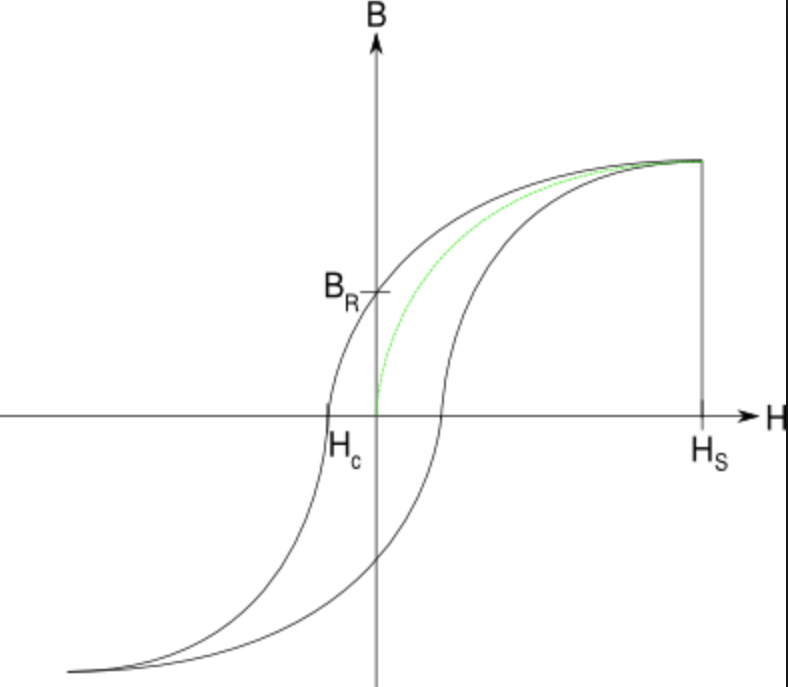
\includegraphics[max width=0.7\linewidth]{/tex/2iteration/billeder/Hysteresekurve.png}
	\caption{Hysteresekurve}
	\label{fig: Hysteresekurve}
\end{figure}
\textbf{Tænker teorien her er lidt tynd, eller er det nok??}

\subsection{Design}
Først og fremmest findes ripplestrømmen, som skal løbe i transformatoren. Her er der taget udgangspunkt i, at designe den efter $60\percent$ af udgangsstrømmen. Dette er et tradeoff mellem størrelsen på ripplen og hvor høj en induktans vi får i viklingerne. Større induktans kræver flere vindinger og giver dermed mere tab.
\begin{equation}
I_{ripple} = 0.6 \cdot \frac{V_{out} \cdot I_{out}}{V_{inmaks} \cdot   D_{min}} = 2.13A
\end{equation}
Den nødvendige induktans det kræver for at transformatoren kan rampe op til den nødvendige strøm inden for dutycyclen, udregnes på følgende måde:
\begin{equation}
L = \frac{V_{inmin} \cdot D_{min}}{I_{ripple} \cdot f_s} = 69.43\micro H
\end{equation}
Som beskrevet tidligere skal kernen kunne opbevare den energi som kommer fra primær viklingen, når transistoren er on, for at undgå mætning. Mængden af energi i primærviklingen udregnes ved:
\begin{equation} \label{Primary_energy}
w = \frac{1} {2} \cdot L \cdot {I_{pk}}^2 = 1.083\milli J
\end{equation}
For at beregne den tilladelige mængde energi i transformatoren, skal kernen og kernematerialet kendes. Valget er her faldet på en RM8 kerne og materialet 3f3. RM8 kernens mål gør, at den lige akkurat kan være på printet højdemæssigt. Derudover har Terma tidligere brugt RM8 kerner med 3f3 og har nogle mere præcise mål på AL og air gaps, end der er på datasheets’ne. (Kræver det flere argumenter?)


\noindent Den effektive volumen Ve aflæses for RM8. På databladet for 3f3 aflæses et maks peak af B-feltet til omkring $250\milli T$. Hvis der designes efter, at transformatoren vil operere med et højere B-felt, vil det risikeres at kernen går i mætning. Yderligere findes permeabiliteten for 3f3 materialet uden luftgab. Med disse oplysninger vil transformatoren kunne opbevare følgende energi:
\begin{equation} \label{Energy_no_gap}
w_{kerne} = \frac{1} {2} \cdot \frac{1}{\micro_e} \cdot B^2 \cdot V_e = 53\pico J
\end{equation}
Det er tydeligt at den nødvendige energi på ingen måde kan opbevares i kernen. Da ferrit kan opbevare så lidt energi som det er tilfældet, kan det estimeres at al energien vil blive opbevaret i det luftgap, der designes. Derfor kan permeabiliteten ses som $\micro_0$ i den nye beregning. Den effektive volumen deles op i luftgap og $Al$, så luftgapet kan isoleres. Med dette kan luftgapet beregnes: 
\begin{equation} \label{Airgap}
l_g = \frac{L \cdot {I_{pk}}^2 \cdot \micro_0}{B^2 \cdot A_0} = 690.98\micro m
\end{equation}
Med den ripplestrøm der i første omgang er benyttet, skal der bruges et air gap på ca. $691\micro m$. Den nærmeste air gaps værdi for 3f3 ligger på $488\micro m$ hvilket giver en Al på $160\nano H$. (Dette er ikke databladets værdi, men en værdi der er blevet givet fra Terma, som har testet databladets værdier til ikke at være korrekte.) Det vil ikke fungere, derfor udregnes en induktans, der passer til det air gap i stedet: 
\begin{equation}
L_1 = \frac{l_g \cdot B^2 \cdot A_0}{{I_{pk}}^2 \cdot \micro_0} = 49.035\micro H
\end{equation}
Med kendt Al og induktans kan vindingstallet beregnes. Da der i 2. iteration bruges en 1:1 transformator er dette både for primær og sekundær vikling:
\begin{equation} \label{N}
N = \sqrt{\frac{L_1}{A_L}} = 17.5 \approx 18
\end{equation}
Det passer fint med 18 viklinger på hver side, hvor induktansen igen bliver lidt anderledes når vindingstallet rundes op. 
\begin{equation} \label{L1}
L_2 = N^2 \cdot A_L = 57.76 \micro H
\end{equation}
Med fastlagt induktans kan ny ripple- og peak strøm beregnes.
\begin{equation}
I_{ripple} = \frac{V_{inmin} \cdot D_{max}}{L_2*f_s} = 2.24A
\end{equation}
\begin{equation}
I_{pk} = \frac{V_{out} \cdot I_{out}}{V_{inmin} \cdot D_{maks}} + \frac{I_{ripple}}{2} = 5.64A
\end{equation}

\subsection{Simulering}
I Pspice er kernen og materialet afprøvet, hvor resten af kredsløbet har været med ideele komponenter, for at kontrollere strømme og B-H kurve. Her ses den pspice-model af kernematerialet som bruges:
\begin{figure}[H]
	\center
	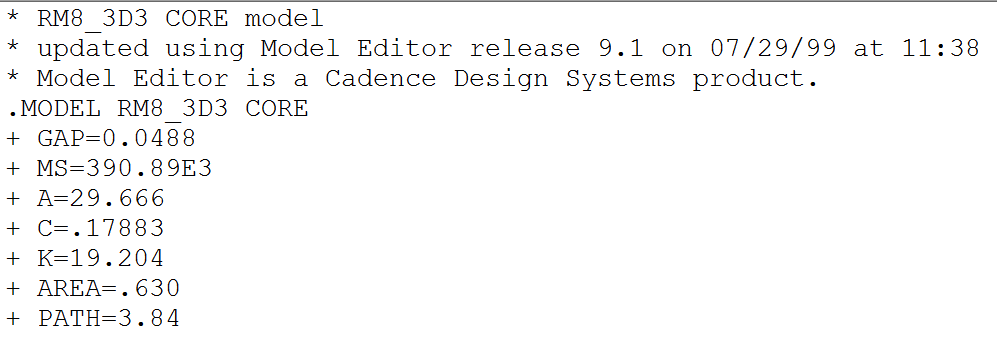
\includegraphics[max width=0.7\linewidth]{/tex/2iteration/billeder/Kernemodel.png}
	\caption{Kernemodel for RM8 3f3}
	\label{fig: Kernemodel}
\end{figure}
Kernemodellen for en 3f3 kerne er indsat, hvor det udregnede air gap også er indtastet. Derudover er der 19 vindinger på primær og sekundærspole. Ellers ingen ændringer i forhold til den rent ideele simulering. Først ses simuleringen af strømmene i transformatoren på primær og sekundær side.
\begin{figure}[H]
	\center
	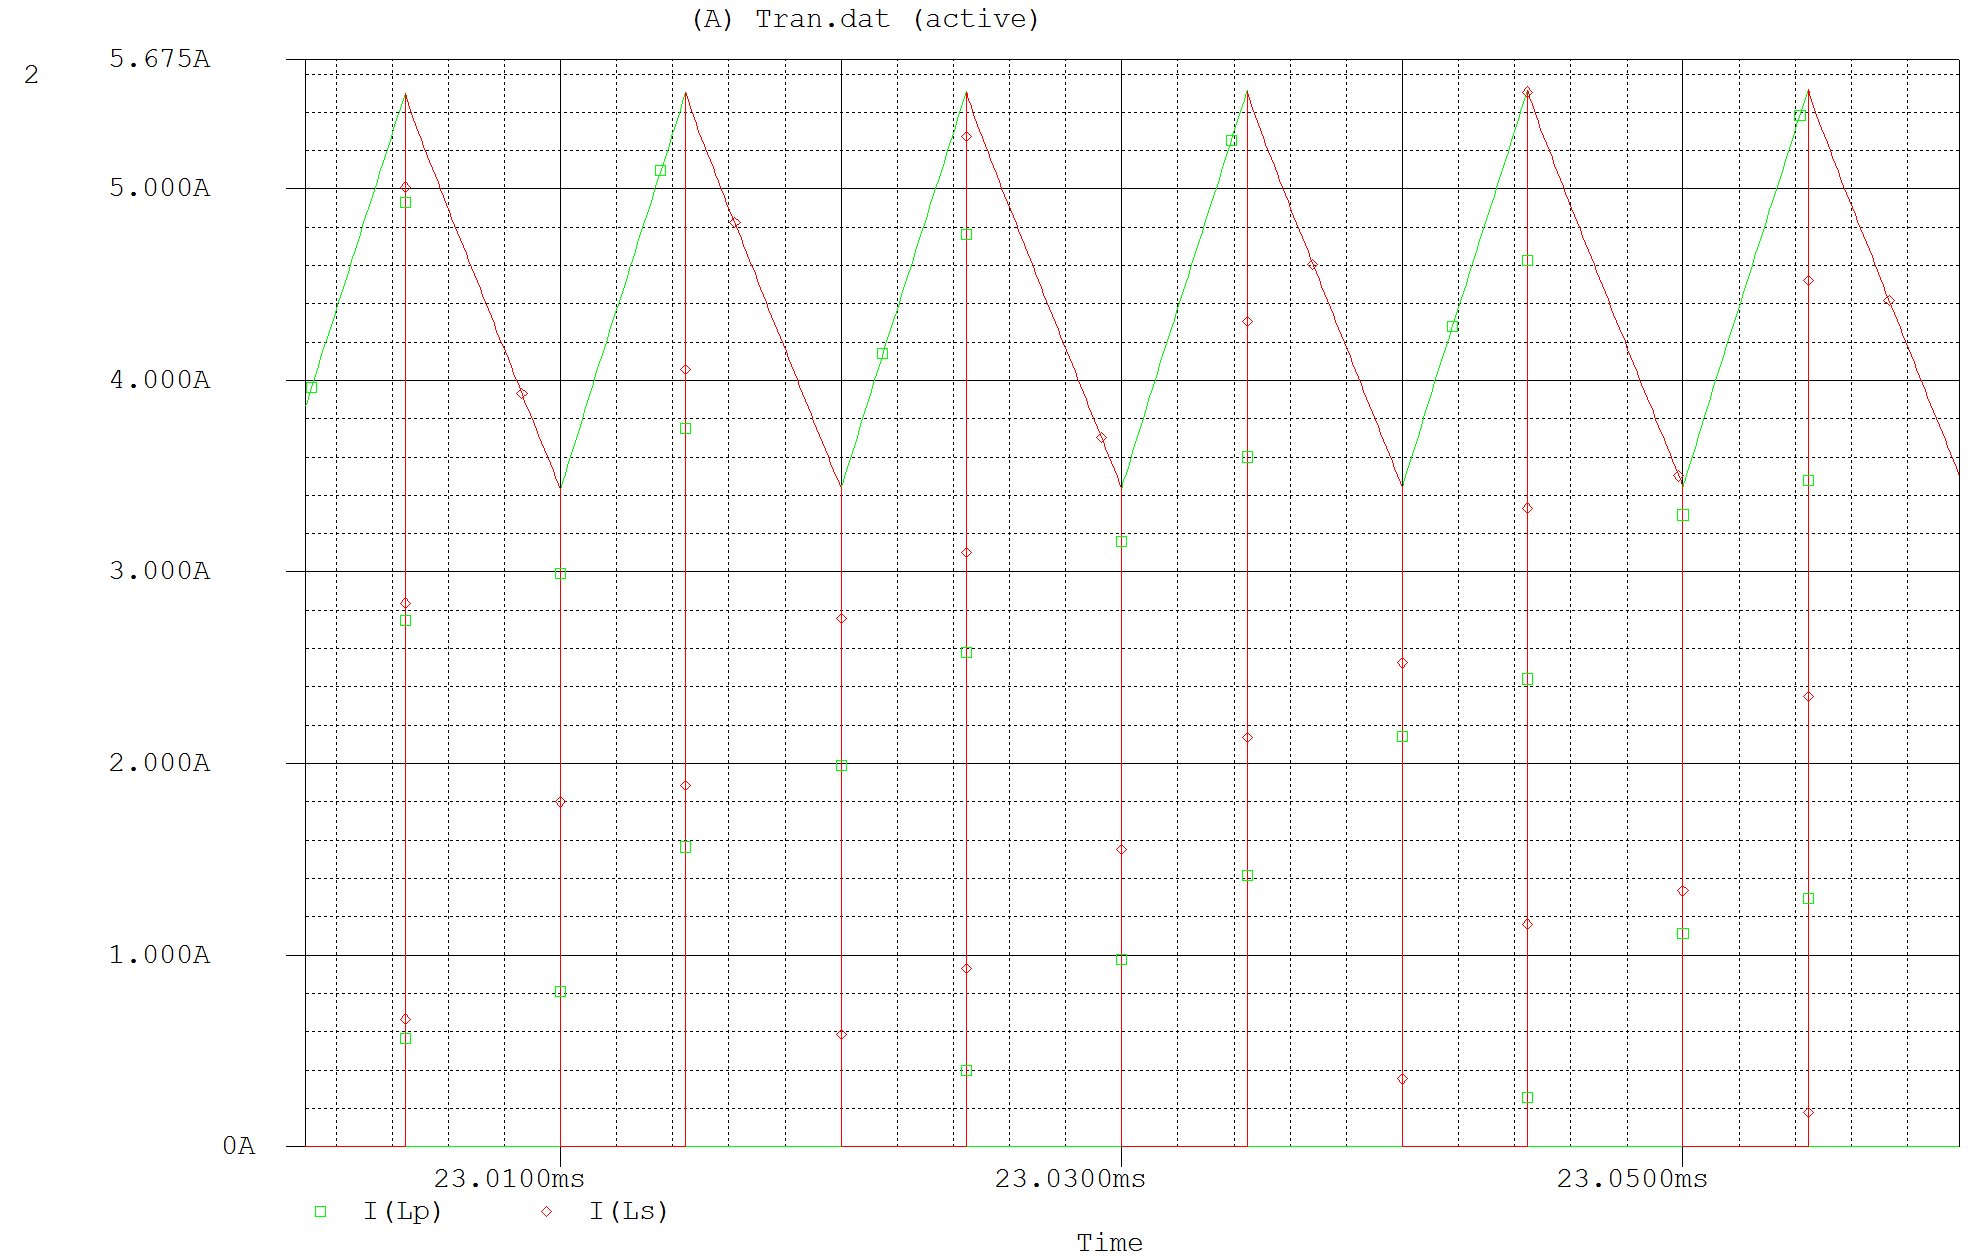
\includegraphics[max width=0.7\linewidth]{/tex/2iteration/billeder/Strom_pri_sek.png}
	\caption{Strøm i primær- og sekundærvikling}
	\label{fig: prisek_strom}
\end{figure}
Det ses tydeligt, at der som ventes køres i CCM, da ripplestrømmene ikke når ned til 0. Ripple- og peak strøm er, som det ses, ens for primær og sekundær, og aflæses til hhv. $2.27A$ og $5.69A$. Det passer fint med det udregnede på $2.24A$ og $5.64A$.
På figur~\ref{fig: RMS_trans} ses RMS strømmene:
\begin{figure}[H]
	\center
	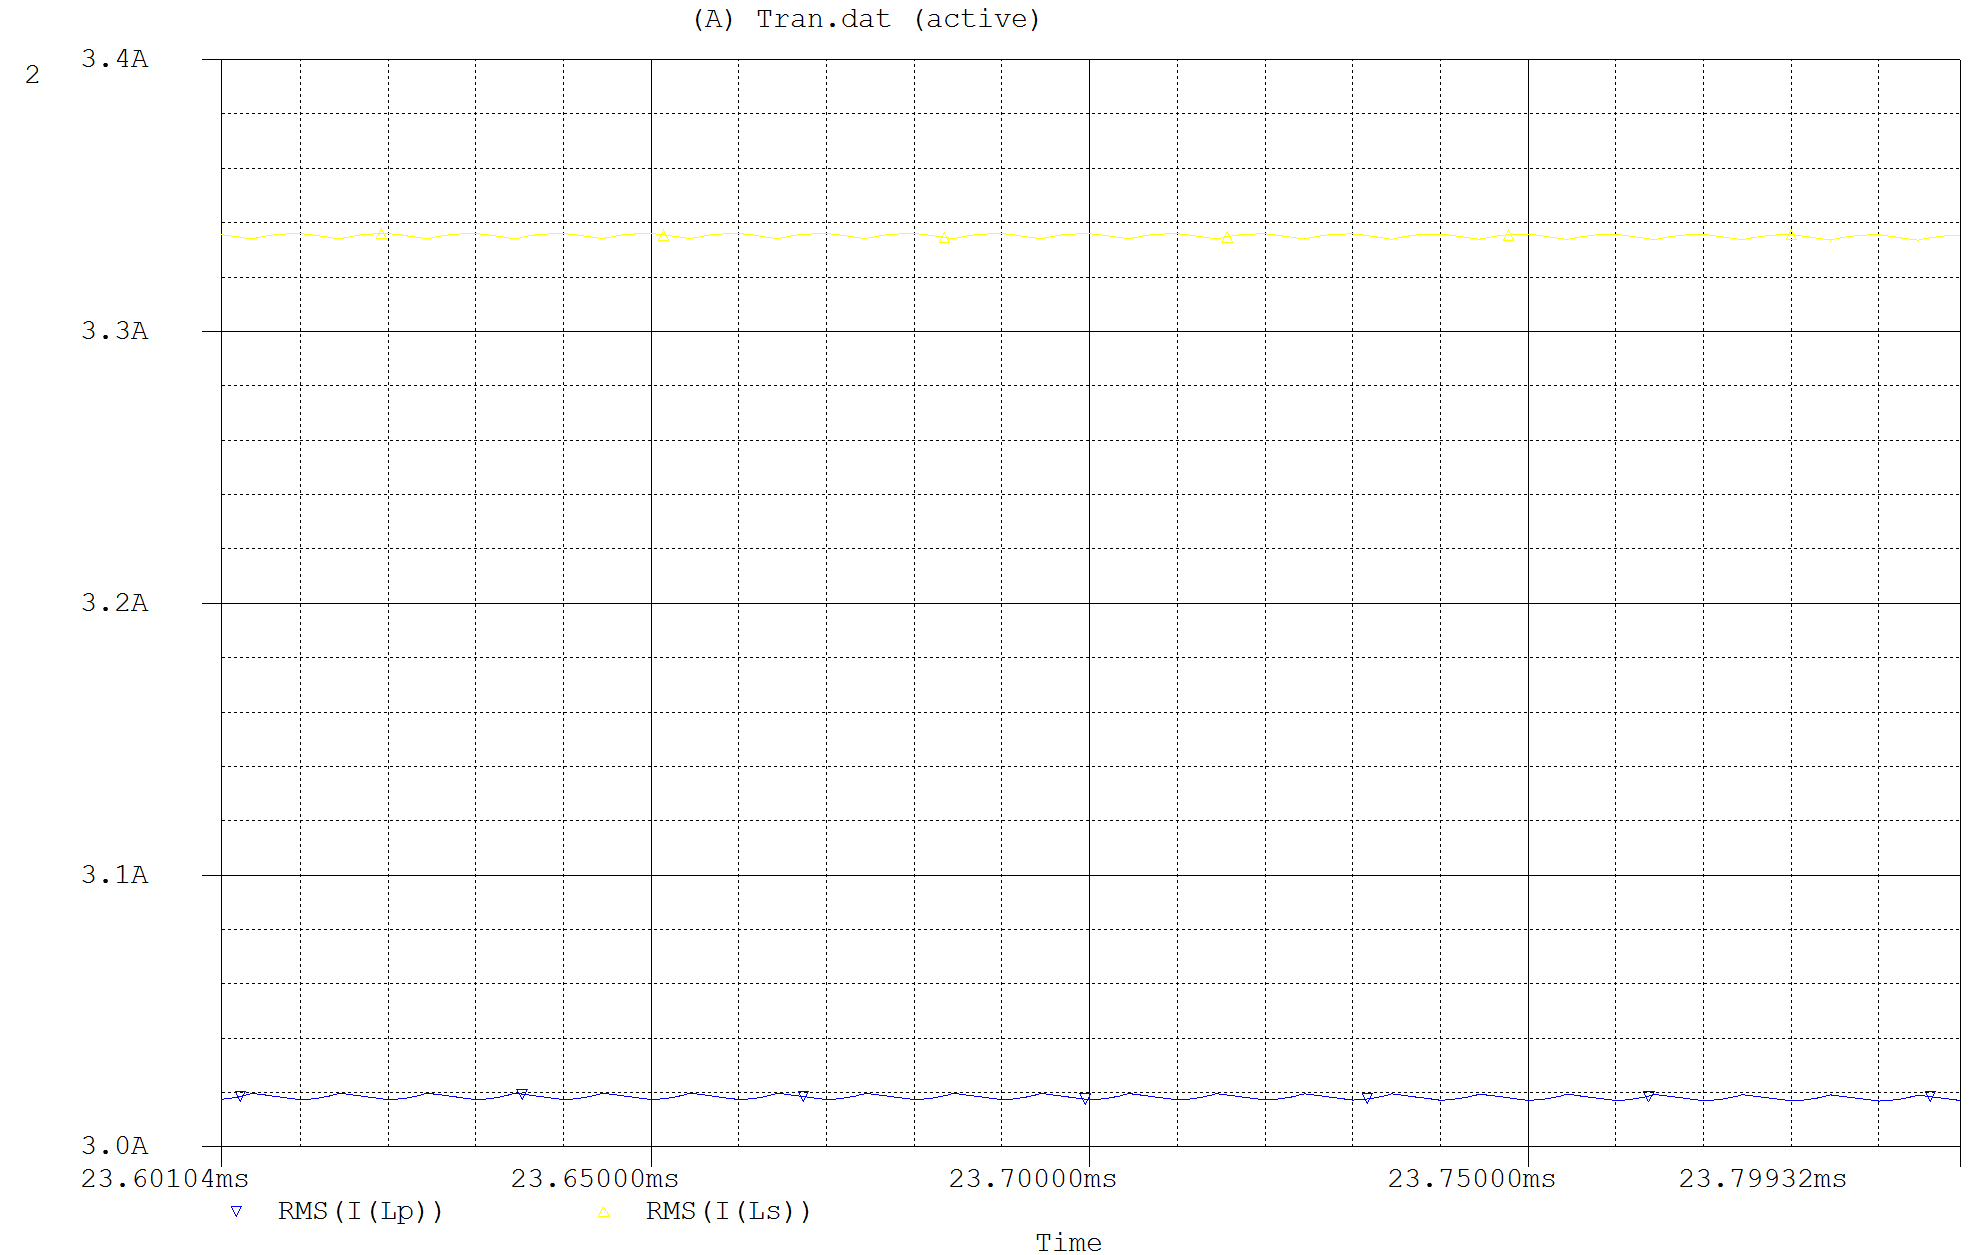
\includegraphics[max width=0.7\linewidth]{/tex/2iteration/billeder/RMS_transformator.png}
	\caption{RMS strømme i transformator (blå=primær og gul=sekundær)}
	\label{fig: RMS_trans}
\end{figure}
Her aflæses den primære til $3.01A$ og den sekundære til $3.33A$, hvilket igen stemmer godt overens med det beregnede på $3.02A$ og $3.36A$.


\noindent Herefter kigges på hysteresekurven, og sikres at den ikke kommer langt over de $250\milli T$, som der er designet efter:
\begin{figure}[H]
	\center
	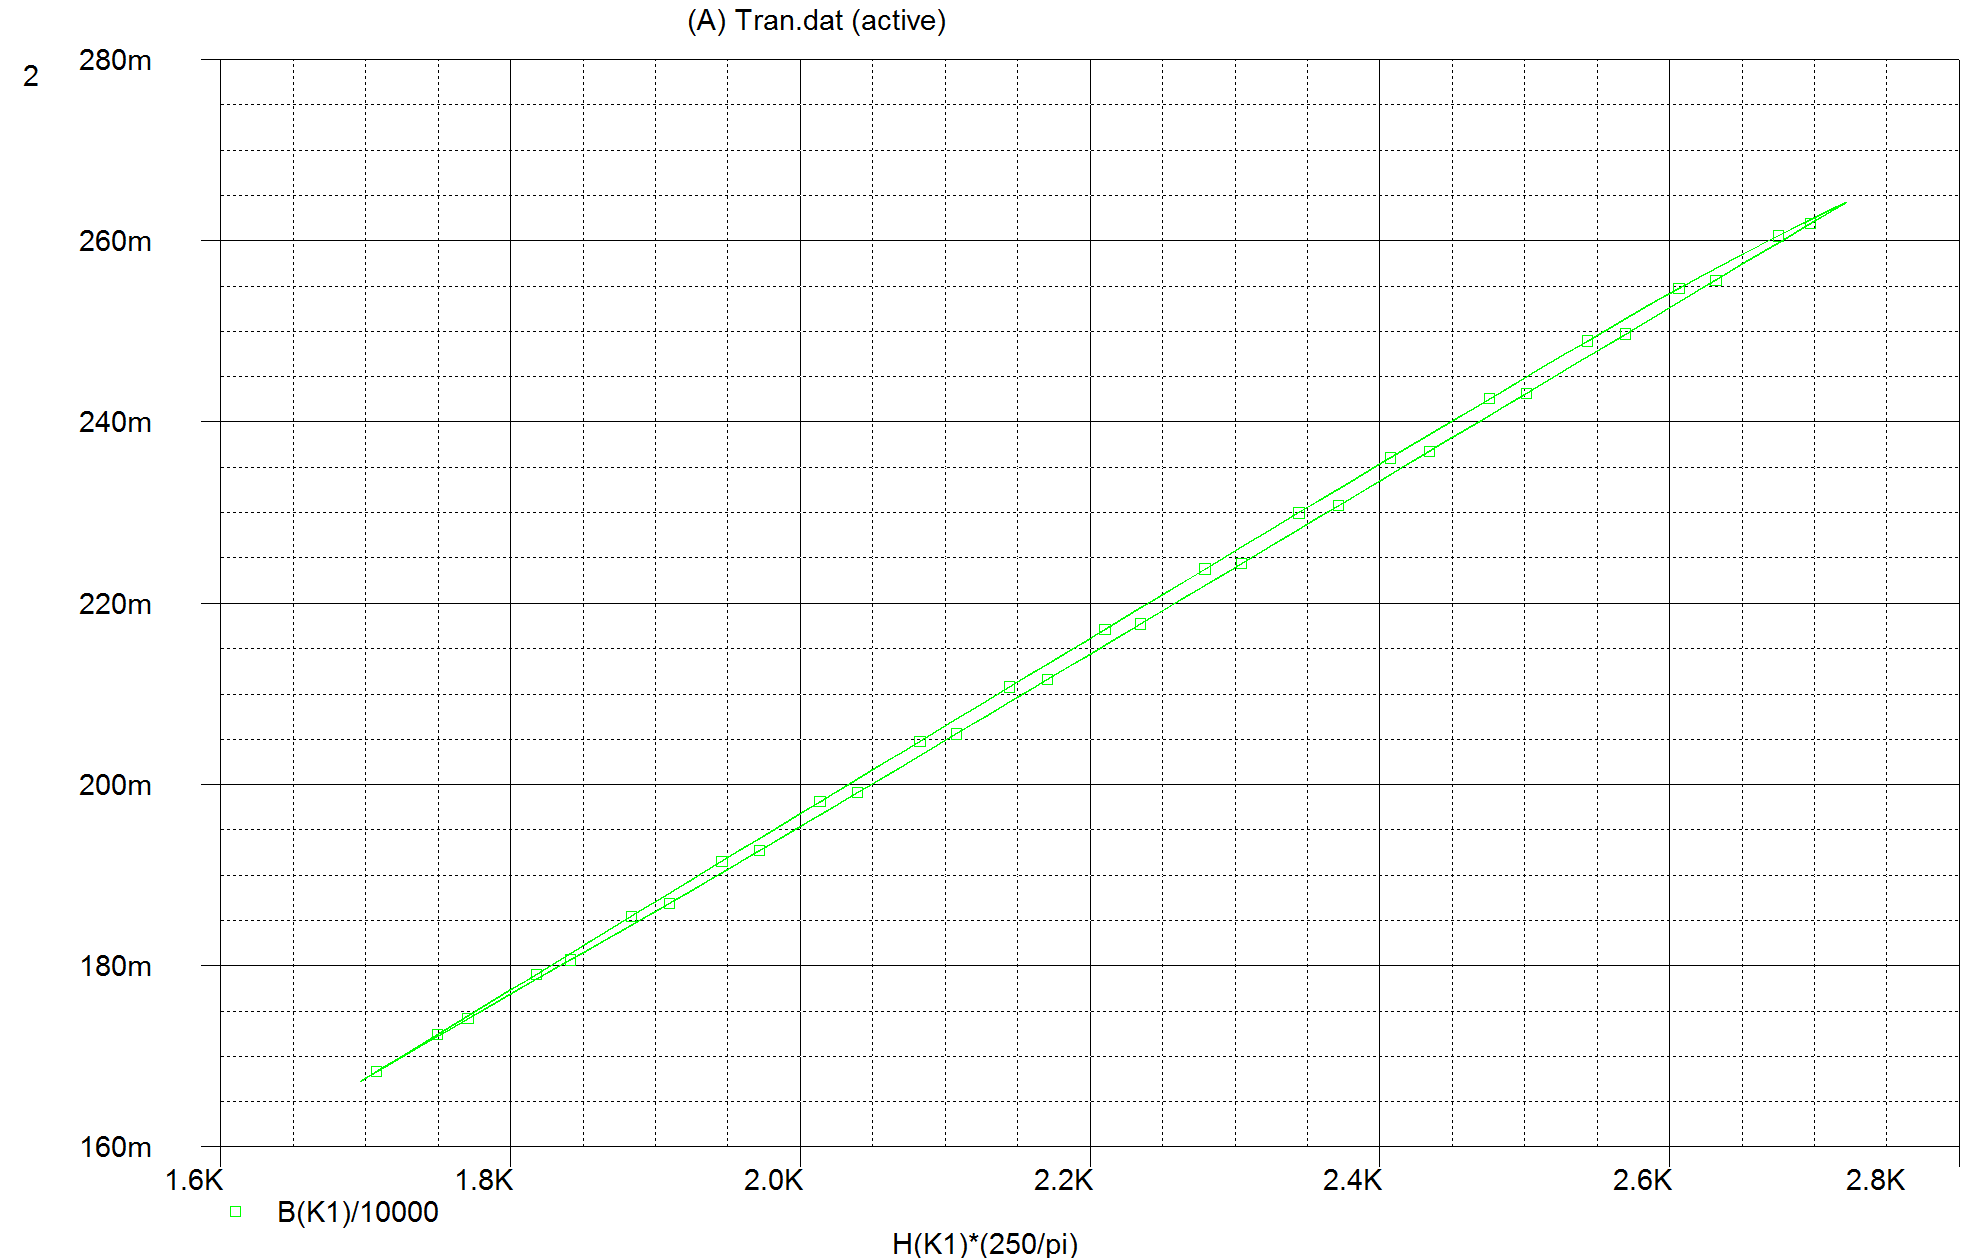
\includegraphics[max width=0.7\linewidth]{/tex/2iteration/billeder/Hysterese_trans.png}
	\caption{Hysteresekurve for transformatoren}
	\label{fig: Hysterese_trans}
\end{figure}
Peak fluxen ligger på ca. $265mT$ hvilket igen passer fint med det der er designet efter. Yderligere ville det kunne ses i toppen og bunden af kurven, hvis den gik i mætning, hvilket den ikke gør her.
Tabet i selve kernen er simuleret ved at tage effekten ved den primære vikling i forhold til den sekundære vikling. Tages der i pspice en average af dette fås nedenstående kurve:
\begin{figure}[H]
	\center
	\includegraphics[max width=0.7\linewidth]{/tex/2iteration/billeder/tabkerne.png}
	\caption{Simuleret kernetab i transformator}
	\label{fig: Kernetab}
\end{figure}
Tabet er simuleret til at ligge ved ca. $310\milli W$

\subsection{Vikling af transformator}
Det er vigtigt at prøve at udnytte kernens mål fuldt ud når vindingerne vikles. Med RM8 kernen er der en bredde på $8.6\milli m$ og en højde på $3.475\milli m$. Ved 2. iteration forsøges de mål udnyttet bedst muligt.
Først udregnes den nødvendige diameter af tråden, når der skal ligge 18 vindinger per lag. 
\begin{equation} \label{d_trad}
d_{tråd} = \frac{8.6\milli m}{18} = 0.478\milli m
\end{equation}
Dette er dog den samlede diameter, altså inklusiv isolering. Der benyttes en isolering med grade 2, som giver en diameter på ledningen eksklusiv isolering på $0.425\milli m$.(HENVISNING) Transformeren er 1:1, så både primær og sekundær vikles med 18 vindinger per lag. Et lag af hver giver en højde på $0.956\milli m$. Altså ikke i nærheden af de $3.475\milli m$ i højden. Derfor vikles 2 ekstra viklinger i parallel for både primær- og sekundærsiden og får dermed den tredobbelte højde. Der indsættes tape mellem hver af de parallelle viklinger. Det giver samlet en højde på $2.867\milli m$ plus tape. Det giver i alt 6 lag, 3 for primær og 3 for sekundær. Overblikket over viklingen kan ses på nedenstående tegning:
\begin{figure}[H]
	\center
	\includegraphics[max width=0.7\linewidth]{/tex/2iteration/billeder/viklingsoverblik.png}
	\caption{Overblik over viklingsantal og tykkelse}
	\label{fig: viklingsoverblik}
\end{figure}
\noindent Tegnes bunden af transformatoren fås der et overblik over, hvordan viklingerne vikles. Det ses, at primær begynder og slutter i samme sidde af transformatoren, mens sekundær vikles fra den anden side.  
\begin{figure}[H]
	\center
	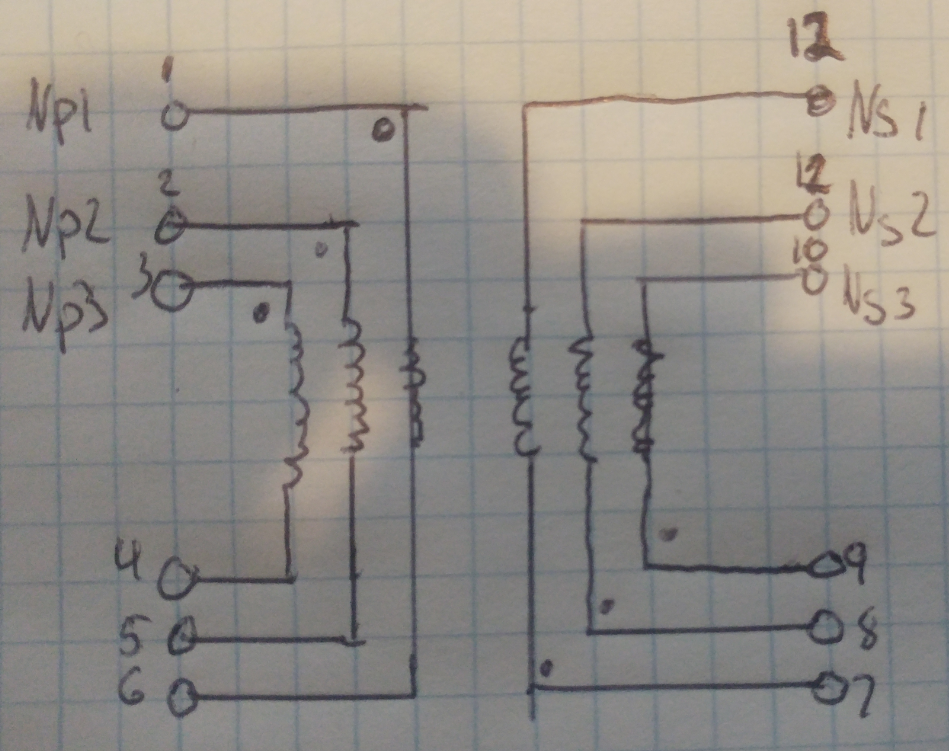
\includegraphics[max width=0.7\linewidth]{/tex/2iteration/billeder/Viklingsbegyndelse.png}
	\caption{Overblik over hvordan viklingerne vikles}
	\label{fig: viklingsbegyndelse}
\end{figure}
\noindent Sidste billede viser hvilken retning der vikles. Her vil primær og sekundær vikles modsatte vej af hinanden, for at få den modsatte polaritet som ønsket.
\begin{figure}[H]
	\center
	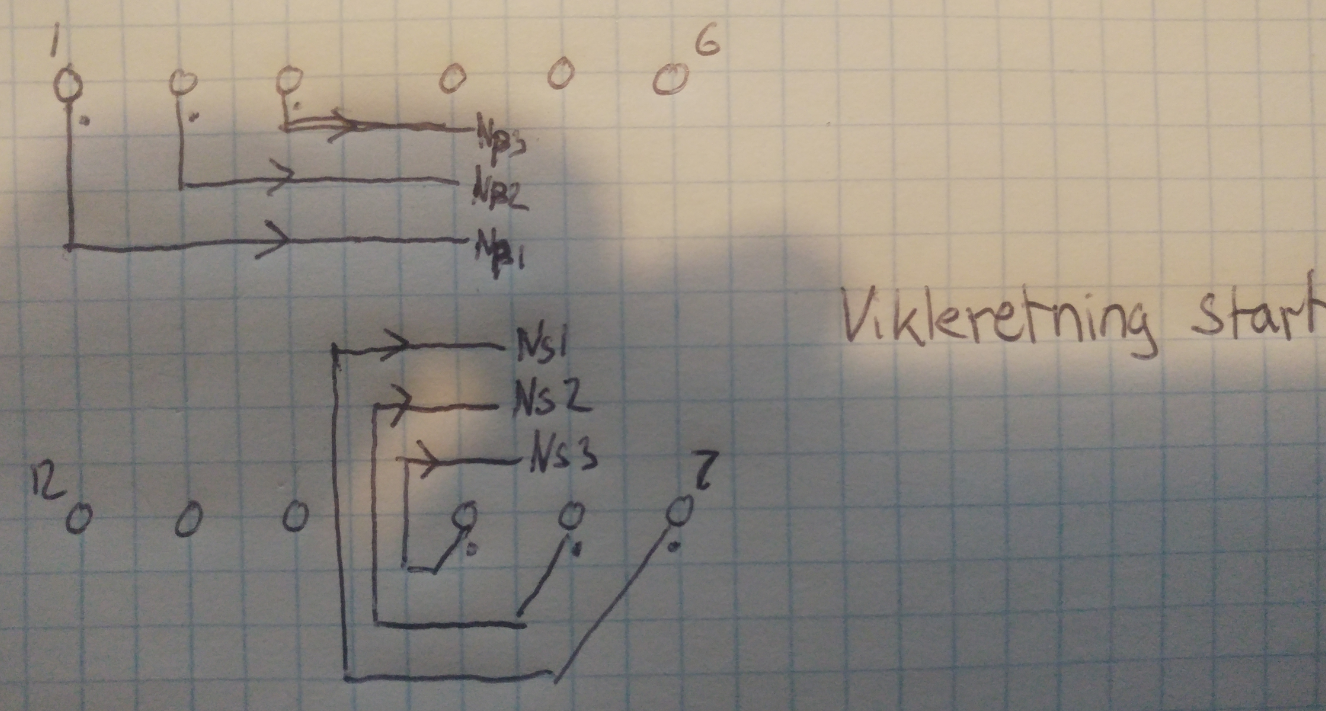
\includegraphics[max width=0.7\linewidth]{/tex/2iteration/billeder/Viklingsretning.png}
	\caption{Begyndelses retning for primær og sekundær}
	\label{fig: viklingsretning}
\end{figure}

\subsection{Realisering}
\begin{figure}[H]
	\center
	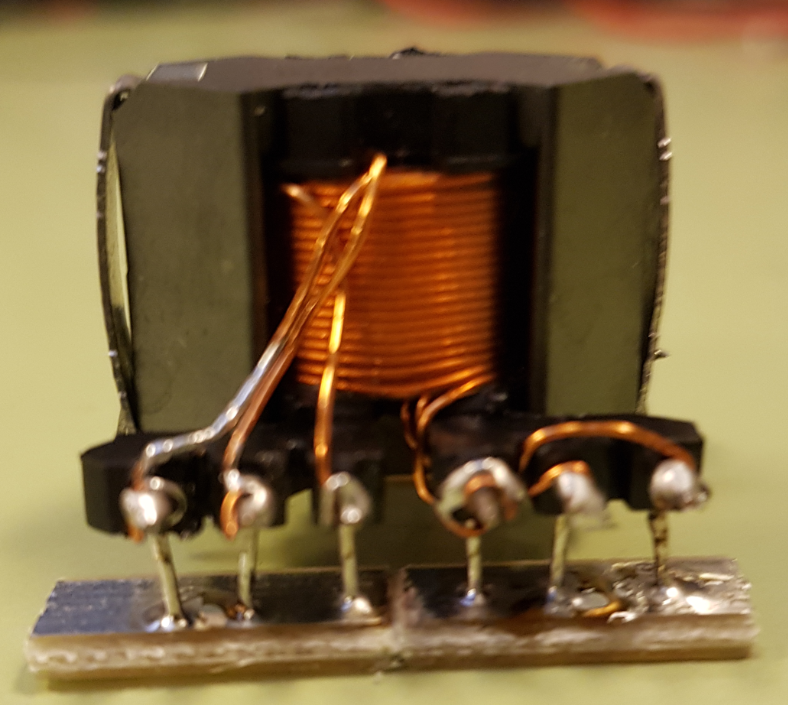
\includegraphics[max width=0.7\linewidth]{/tex/2iteration/billeder/Viklet_transformator.PNG}
	\caption{Viklet transformator}
	\label{fig: Viklettrans}
\end{figure}
På figur~\ref{fig: Viklettrans} ses den viklede transformator. Ved viklingen måtte det erkendes, at der ikke kunne presses 18 vindinger ind, med en ledningstykkelse på $0.450\milli m$, som ellers i forvejen var mindre end den udregnede tykkelse på $0.478\milli m$. I stedet benyttes en tykkelse på $0.425\milli m$ og der tilføjes en ekstra vikling, så det totale antal vindinger ender på 19 per vikling. (ER VI SIKRE PÅ DET IKKE NETOP ER DEN TRÅD VI HAR FÅET?? At trådtykkelsen der står er uden isolering?)

\noindent \textbf{Endelig induktans}


\noindent Da vindingstallet blev 19 i stedet for de 18, er induktansen lidt højere end beregnet i første omgang. Den endelige induktans den viklede transformator beregnes til:
\begin{equation} \label{L_2}
L_2 = N^2 \cdot A_L = 57.76\micro H
\end{equation}
Det ændrer igen en smule på ripple- og peak strømmen i transformatoren:
\begin{equation} \label{I_ripple_final}
I_{ripple} = \frac{V_{inmin} \cdot D_{max}}{L_2*f_s} = 2.01A
\end{equation}
\begin{equation} \label{I_pk_final}
I_{pk} = \frac{V_{out} \cdot I_{out}}{V_{inmin} \cdot D_{maks}} + \frac{I_{ripple}}{2} = 5.53A
\end{equation}

\subsection{Test af transformator}
Transformatoren er testet ved at måle både selvinduktionen i primær- og sekundærviklingerne samt spredningsselvinduktionen. Til dette blev en impedansmåler brugt. 


\noindent Til sådan en måling er det vigtigt, at gøre ledningerne så korte som muligt, da der vil skabes yderligere induktans i dem. Derfor ses ved opstillingen på figur~\ref{fig: Transopstilling} de meget korte ledninger samt at der bliver brugt en 4-wire teknik. Det vil sige to ledninger på hver side af det der måles på. Det gør at strømmen kan sendes igennem det ene sæt ledninger, mens der måles med det andet sæt. Da der ikke sendes en strøm igennem det sæt der måles på, undgås den induktive fejlmåling, der ellers vil komme fra ledningerne. 

\begin{figure}[H]
	\center
	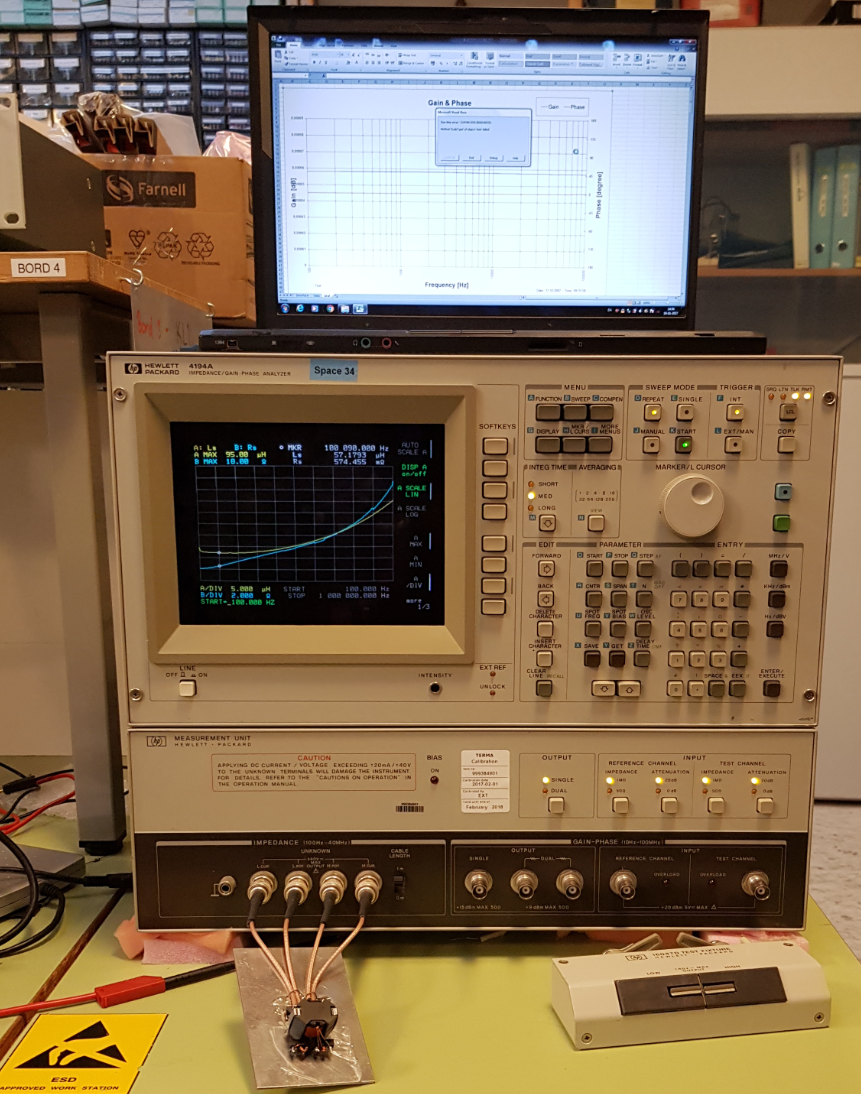
\includegraphics[max width=0.7\linewidth]{/tex/2iteration/billeder/Samlet_transformatortest_opstilling.PNG}
	\caption{Samlet transformatortest opstilling}
	\label{fig: Transopstilling}
\end{figure}

\noindent Måleresultaterne tages med USB ud af impedansmåleren og indsættes i et Excel ark.  

\noindent Selve impedansmåleren havde et lille offset på målingerne. Derfor blev der først lavet en kalibreringsmåling, hvor ledningerne alle målte samme sted. Offsettet herfra er i Excel trukket fra de efterfølgende målinger.    

\noindent Herefter måles der på de 2 sider af primærviklingen, mens sekundærsiden holdes åben. På denne måde fås induktansen i den primære vikling. Da transformatoren er 1:1, er det også induktansen i den sekundære vikling. 
\begin{figure}[H]
	\center
	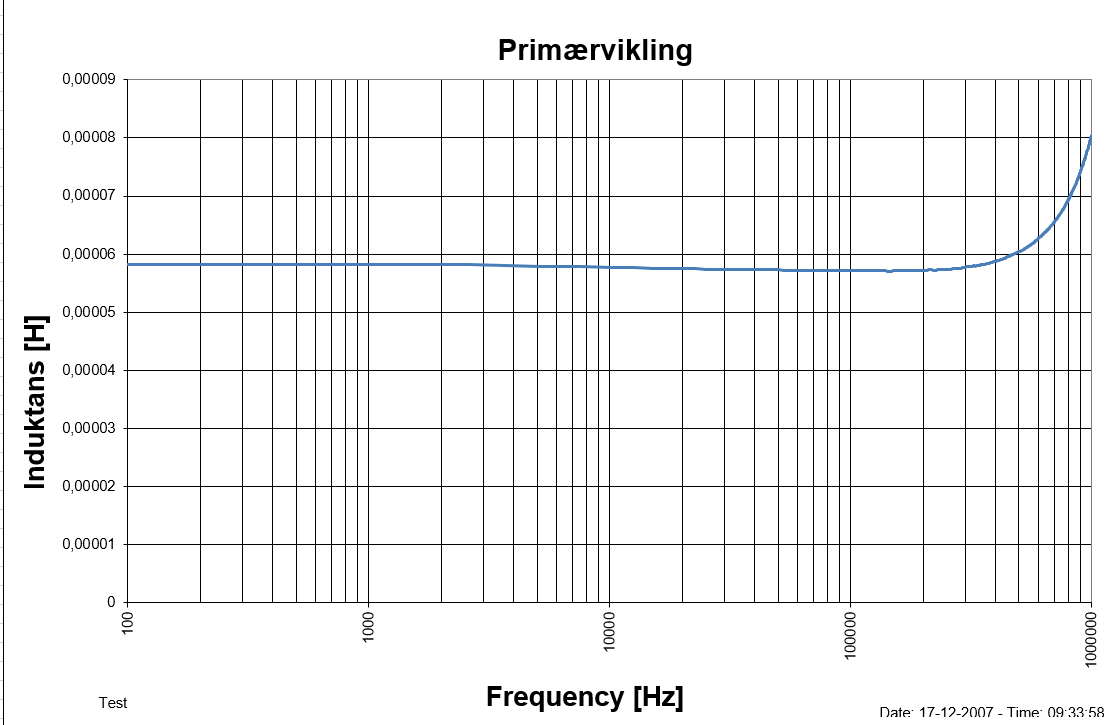
\includegraphics[max width=0.7\linewidth]{/tex/2iteration/billeder/Primarinduktans.png}
	\caption{Målt induktans i primær vikling}
	\label{fig: Primarinduktans}
\end{figure}
\noindent Her er målingen plottet med et frekvenssweep fra $100Hz$ til $1\mega Hz$. Ved de meget høje frekvenser ses det, at kapacitive parasitter tager over. Den skal benyttes omkring 100kHz og her fås værdien i Excel til $57.7\micro H$, hvilket er præcis den induktans der skulle opnås. De præcise målinger kan ses i Excel dokumentet ”Inductance primærvikling” i bilagsmappen. 
Spredningsselvinduktionen fås ved, at kortslutte den sekundære vikling, mens der igen måles hen over den primære vikling. I en ideel transformator bør der her måles 0. Derfor vil induktansen målt her, svare til spredningsselvinduktionen. På samme måde som før er måleresultaterne sendt til Excel hvorudfra en graf kan tegnes. De præcise målinger kan ses i Excel dokumentet ”Spredningsselvinduktion” i bilagsmappen:
\begin{figure}[H]
	\center
	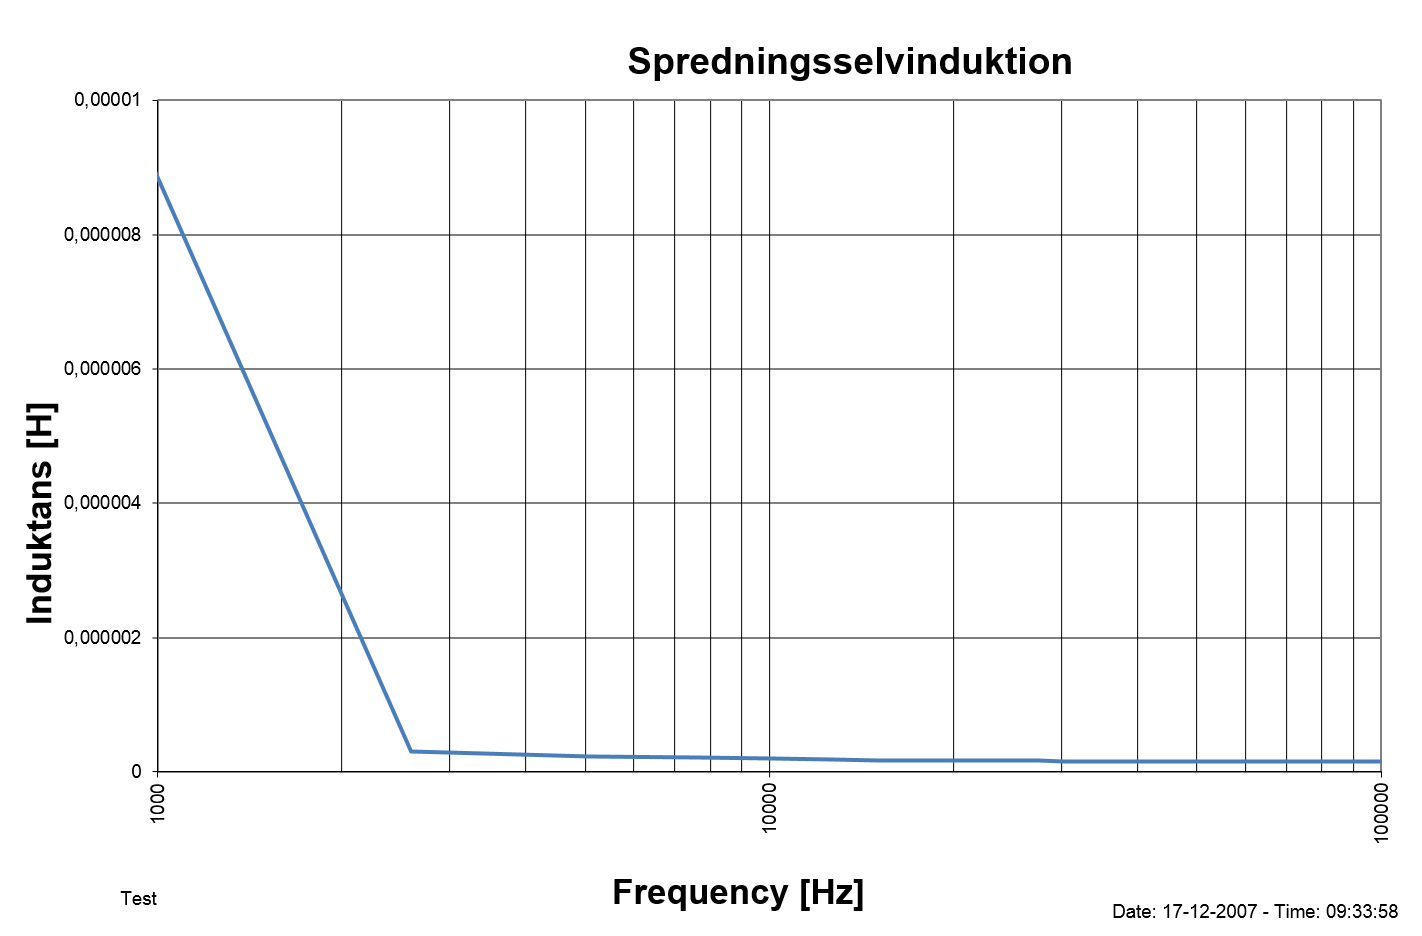
\includegraphics[max width=0.7\linewidth]{/tex/2iteration/billeder/Spredningsselvinduktion.png}
	\caption{Målt spredningsselvinduktion i transformator}
	\label{fig: leakageinductance}
\end{figure}
\noindent Denne graf er fået ud fra et frekvenssweep fra 1kHz til $100\kilo Hz$. Ved de $100\kilo Hz$ er spredningsselvinduktionen på $152\nano H$, hvilket er den værdi der bruges. 

% Dokumentation af PWM-controller %
% UCC1801 %

\section{PWM-controller} \label{PWM}
PWM-controlleren er en vigtig del af en SMPS. Det er den der står for tilpasningen af switch-signalets duty-cycle, således udgangen holdes stabilt, når inputtet påvirkes eller ændres. Det er vigtigt at vælge PWM-controller ud fra kravene til converteren. PWM-controllere er ofte begrænset til en maksimal duty-cycle på enten $50\percent$ eller $100\percent$. Derudover skal der vælges, hvilken form for regulering af converterens udgangstrin der ønskes, da controlleren skal understøtte dette. 

Ud fra beregningerne af den maksimale duty-cycle i afsnit~\ref{maksimum_duty_cycle}, vælges det at PWM-controlleren maksimalt skal have en duty-cycle på $50\percent$. For at kunne opnå en mere præcis regulering, vælges det at bruge peak-current regulering. Denne form for regulering, regulerer efter peak-strømmen i transformatorens primærvikling. Da den regulere efter dette, opnås der også en strømbegrænser i regulerings-loopet. Ud fra disse krav vælges en PWM-controller af typen UCC1801\cite{UCC1801}. Det er en controller Terma har erfaring med, og derfor også nemt kan udskiftes med en space-godkendt controller.

\subsection{Funktionalitet}
På figur~\ref{fig:PWM_block_diagram} ses et funktionelt block diagram over UCC1801. Det indeholder controllerens overordnede komponenter, og giver et overblik over dens funktionalitet. 

\begin{figure}[H]
	\center
	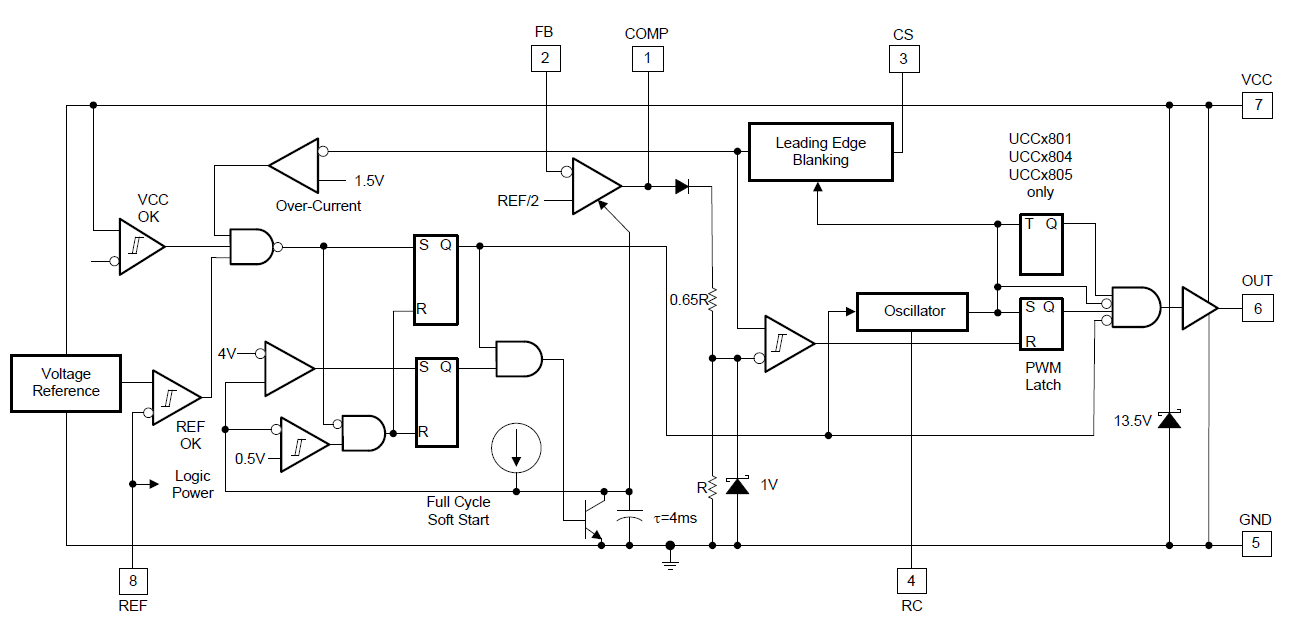
\includegraphics[max width=0.9\linewidth]{/tex/2iteration/billeder/PWM_block_diagram.PNG}
	\caption{UCC1801 - Funktionelt Block Diagram}
	\label{fig:PWM_block_diagram}
\end{figure}

Tabel~\ref{tab:ucc1801_specs} viser de mest essentielle specifikationer for UCC1801, i forhold til en flyback converter. Disse er udvalgte specifikationer fra databladet.

\begin{table}[H] 			
	\centering
	\begin{tabularx}{\textwidth}{|X|c|c|c|} 
		\hline
		\textbf{Specifikation} & \textbf{Min} & \textbf{Typ} & \textbf{Max} \\ \hline
		$V_{CC}$ &  &  & $12V$ \\ \hline
		$I_{out}$ &  &  & $1A$ \\ \hline
		$V_{Reference}$ & $4.925V$ & $5V$ & $5.075V$ \\ \hline
		$D_{max}$ & $48\percent$ & $49\percent$ & $50\percent$ \\ \hline
		$V_{on,th}$ & $8.6V$ & $9.4V$ & $10.2V$ \\ \hline
		$V_{off,th}$ & $6.8V$ & $7.4V$ & $8V$ \\ \hline
		Temperature Range & $-55\degreeCelsius$ &  & $125\degreeCelsius$ \\ \hline
		$f_{osc}$ & & & $1M\hertz$ \\ \hline
	\end{tabularx}

	\caption{Relevante specifikationer for UCC1801}
	\label{tab:ucc1801_specs}
\end{table}


\subsubsection{Ben konfiguration}
Der tages udgangspunkt i en UCC1801, med en PDIP pakke type. Figur~\ref{fig:ucc1801_pin_overview} viser en oversigt over ben konfigurationen for en sådan pakke. Det er en 8-bens IC, hvor samtlige ben bliver brugt. Benenes funktionalitet er overordnet beskrevet i tabel~\ref{tab:ucc1801_pin_functionality}, og vil blive uddybet i de følgende afsnit.

\begin{figure}[H]
	\center
	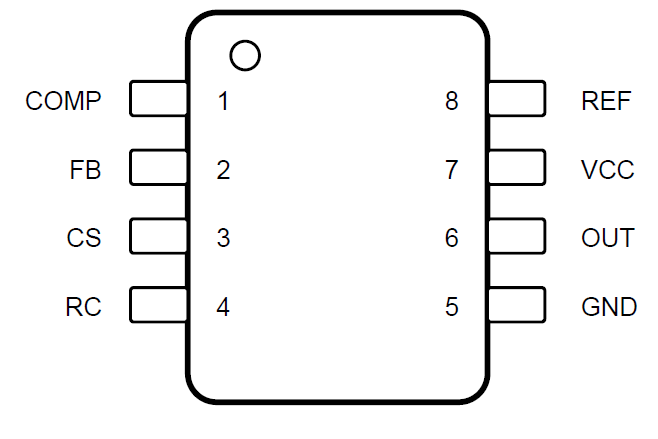
\includegraphics[max width=0.7\linewidth]{/tex/2iteration/billeder/ucc1801_pin_overview.PNG}
	\caption{Ben konfiguration for UCC1801}
	\label{fig:ucc1801_pin_overview}
\end{figure}

\begin{table}[H] 			
	\centering
	\begin{tabularx}{\textwidth}{|c|c|c|X|} 
		\hline
		\textbf{Navn} & \textbf{Ben} & \textbf{I/O} & \textbf{Beskrivelse} \\ \hline
		COMP & 1 & O & COMP er outputtet fra den indbyggede fejlforstærker. Dette ben bruges til at lave et feedback til FB benet i reguleringssløjfen. 	\\ \hline
		FB 	 & 2 & I & FB er inputtet til den indbyggede fejlforstærker. Den er forbundet til den inverterende indgang af forstærkeren. Den bruges sammen med COMP, som en del af reguleringssløjfen.\\ \hline
		CS   & 3 & I & CS er inputtet til current sense komparatorne. UCC1801 har to komparatorere til current sense: PWM komparatoren og overstrøms komparatoren. PWM-komparatoren bruges til, at trække udgangssignalet lavt, når CS-signalet overstiger $1V$. Overstrøms komparatoren er en indbygget overstrømsbeskyttelse. Den tvinger udgangen lav, så længe CS-signalet er over $1.5V$ \\ \hline
		RC 	 & 4 & I & RC er inputtet til oscillatoren. Oscillator frekvensen, og dermed også switch-frekvensen, sættes ud fra tidskonstanten mellem en modstand og en kondensator.  \\ \hline
		GND  & 5 & - & GND er ground for IC'ens komponenter.  \\ \hline
		OUT  & 6 & O & OUT er IC'ens output. Det er et PWM-signal, hvis duty-cycle afhænger af PWM-komparatoren. Outputtet skiftes mellem GND og VCC, hvilket betyder at VCC skal være høj nok, til at drive MOSFET'en.  \\ \hline
		VCC  & 7 & I & VCC er forsyning til IC'ens komponenter. Det foreslås at vælge en høj VCC, for at mindske støjpåvirkninger. For at mindske støj på forsyningen anbefales det, at bypasse VCC med en kondensator på minimum $1\micro \farad$, tæt på IC'en. \\ \hline
		REF  & 8 & O & REF er outputtet for IC'ens interne spændingsreference. Den bruges bl.a. som reference til fejlforstærkeren. Derudover forsyner den IC'ens logiske komponenter. For at mindske støj på referencen, anbefales det at bypasse REF med en kondensator på minimum $1\micro \farad$, tæt på IC'en. \\ \hline
	\end{tabularx}
	
	\caption{Ben funktionalitet for UCC1801}
	\label{tab:ucc1801_pin_functionality}
\end{table}

\subsection{Under Voltage LockOut}
UCC1801 indeholder en Under Voltage LockOut (UVLO) beskyttelse. Dette betyder at forsyningsspændingen skal være et bestemt niveau, før controlleren starter. Som en konsekvens af dette vil både outputtet og referencespændingen holdes lav, indtil grænseværdien er nået. For at have en hysteresemargin, har den både et turn ON og et turn OFF niveau. Ved UCC1801 er disse niveauer $V_{on,th}=9.4V$ og $V_{off,th}=7.4V$. Da amplituden af output-signalet er lig VCC, vil controlleren ikke prøve at drive MOSFET'en før $V_{CC}=9.4V$. Da en MOSFET typisk har en $V_{gs,th}$ mellem $4$ og $5V$, vil der ikke opnås et stadie hvor MOSFET'en kun er delvist ON. Dette ses også på referencespændingen, da den først bliver $5V$ når $V_{CC}\geqslant 9.4V$. Referencen kan derfor også bruges, som en ON/OFF indikator. 

\subsection{Switch-frekvens}
Controllerens switch-frekvens sættes af oscillator blokken i block diagrammet. Den genererer en savtand-spænding, som trigger den efterfølgende latch. Dette giver et PWM-signal, da det skifter mellem VCC og GND.
Stigetiden for savtand spændingen bliver bestemt af tidskonstanten for et eksternt RC-kredsløb. Faldetiden for signalet bliver bestemt af den eksterne kondensator, samt ON-modstanden i en intern transistor. Den on-modstand er opgivet til ca. $130\ohm$. Denne faldetid vil begrænse den maksimale duty-cycle, da outputtet vil være lavt i løbet af faldetiden. 

\begin{figure}[H]
	\center
	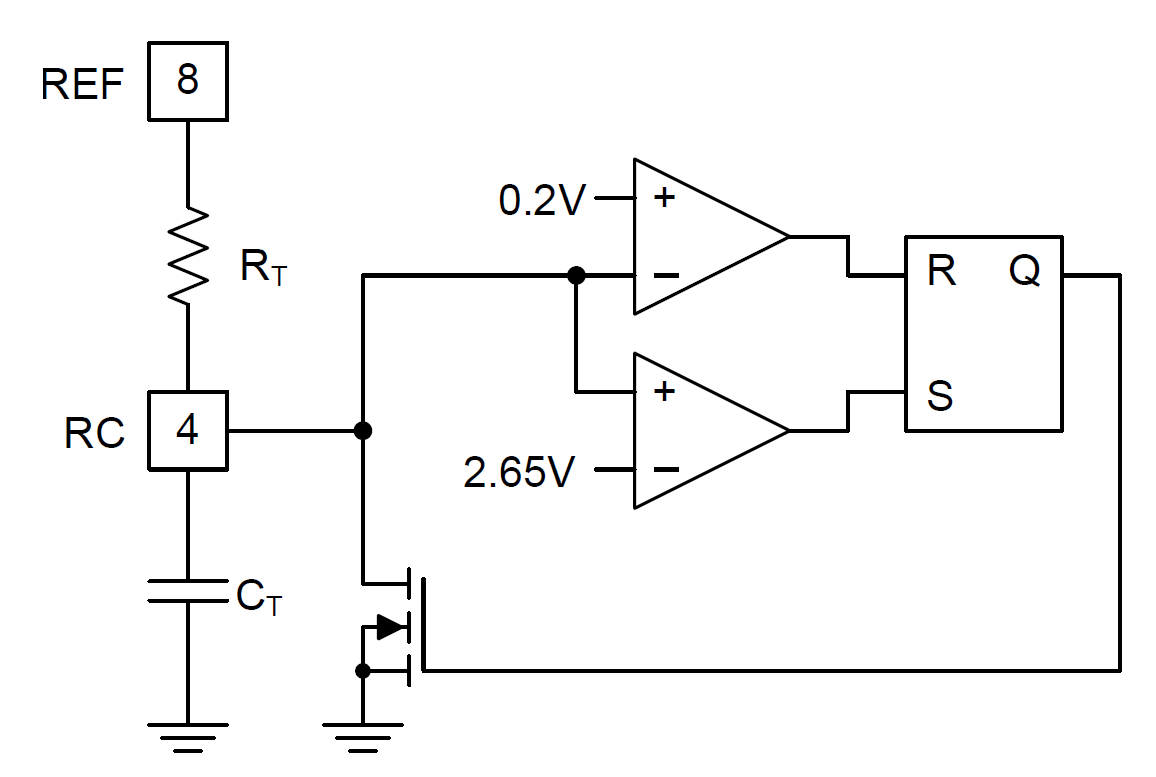
\includegraphics[max width=0.7\linewidth]{/tex/2iteration/billeder/PWM_oscillator_diagram.PNG}
	\caption{Oscillator diagram}
	\label{fig:PWM_oscillator_diagram}
\end{figure}

Figur~\ref{fig:PWM_oscillator_diagram} viser et ækvivalent diagram for oscillator blokken. Komponenterne $R_T$ og $C_T$ er det eksterne RC kredsløb, mens resten er interne komponenter. På diagrammet ses det at operationsforstærkerne er koblet til henholdsvis $0.2V$ og $2.65V$. Dette sætter maksimum og minimum for savtand spændingen. 

Da der skal komme en flanke på output-signalet hver gang savtand spændingen rammer maksimum, skal frekvensen af savtand spændingen være den dobbelte af den ønskede switch-frekvens. Der ønskes en switch-frekvens på $100k\hertz$, derfor sættes oscillator frekvensen til $f_{osc}=200k\hertz$. I databladet er det anbefalet at $R_T$ vælges mellem $10k\ohm$ og $200k\ohm$, mens det anbefales at $C_T$ vælges mellem $100p\farad$ og $1000p\farad$. Formel~\ref{f_osc} er opgivet i databladet og bruges til at estimere RC komponenterne. $C_T$ sættes til $200p\farad$, og $R_T$ beregnes:
\begin{equation} \label{f_osc}
R_{T} = \frac{1.5}{f_{osc} \cdot C_T} = \frac{1.5}{f_{osc} \cdot C_T} = 37.5k\ohm
\end{equation}
Ved et opslag i databladet ses det, at med en $C_T=200p\farad$ kan der maksimalt opnås en duty-cycle på ca. $48.9\percent$. Da converteren maksimalt skal opererer med en duty-cycle på $44.7\percent$, godtages dette.

\subsection{Current sense kredsløb} \label{CS_loop}
Som nævnt i afsnit~\ref{PWM} er der valgt at bruge peak-current regulering. Denne form for regulering består af to reguleringssløjfer - en spændings- og en strømsløjfe. I dette afsnit beskrives dimensioneringen af strøm sløjfen, mens spændingssløjfen beskrives i afsnit~\ref{V_loop}.

Current sense kredsløbet består, som minimum, af en current sense modstand. Denne modstand bruge til at konvertere strømmen i transformatorens primærvikling om til en spænding. Denne konvertering vil gøre, at kurveformen for strømmen og spændingen er ens, dog med en faktor til forskel. PWM-komparatoren i controlleren trigger udgangen, når current sense spændingen er rampet op til $1V$. Derfor skal modstanden dimensioneres således, spændingen over den er lig $1V$ når peak-strømmen i transformatoren er lig $5.53A$. Dette regnes ud fra Ohm's lov:
\begin{equation} \label{R_cs}
R_{cs} = \frac{1V}{5.53A} = 0.181\ohm
\end{equation}

Da den mindste modstandsværdi der er til rådighed er på $1\ohm$, vil der blive brugt $6\cdot 1\ohm$ i parallel. Dette vli give en modstandsværdi på $0.167\ohm$. 



\subsubsection{Filtrering}
På grund af switching-spikes i MOSFET'en, når den går ON, vil der også komme spikes på current sense signalet. Hvis disse spikes når et niveau der er højere end $1V$, vil det trigger komparatoren. Dette vil få controlleren til at generer et PWM-signal, der er meget lavere end det ønskede. Derfor implementeres der et filter, for at filtrere disse spikes væk.

UCC1801 har et indbygget digitalt filter, kaldet Leading Edge Blanking. Dette filter er designet til at filtrere de første $100ns$ af signalet væk, og dermed fjerne spiken. Ideelt set vil dette give et signal, som ses på figur~\ref{fig:ucc1801_leading_edge}.

\begin{figure}[H]
	\center
	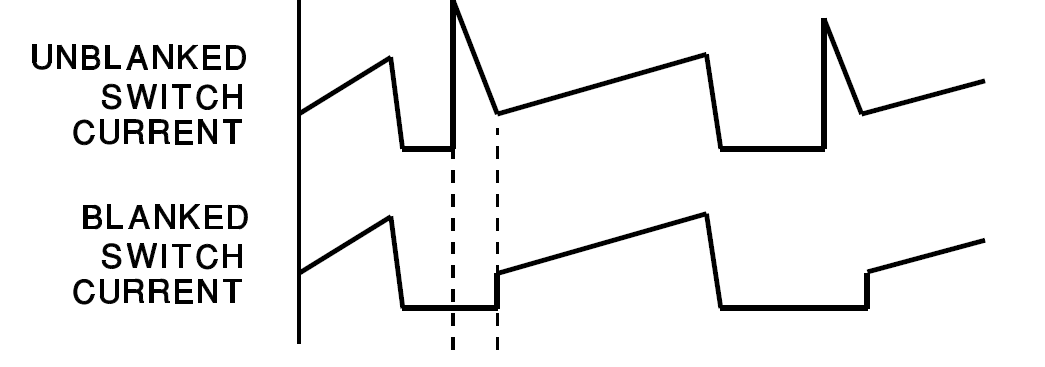
\includegraphics[max width=0.7\linewidth]{/tex/2iteration/billeder/ucc1801_leading_edge.PNG}
	\caption{Current sense signal før og efter Leading Edge Blanking}
	\label{fig:ucc1801_leading_edge}
\end{figure}

Det digitale filter er ikke altid tilstrækkeligt, og derfor designes et eksternt analogt RC-filter, for yderligere filtrering. Det designes til at have en stige tid på $300ns$, for at tilføje en yderligere filtrering på ca. $200ns$. 

\noindent Med en stige tid på $300ns$, kan båndbredden af filteret estimeres:
\begin{equation} \label{filter_BW}
BW \approx \frac{0.34}{t_r} \approx 1.133M\hertz
\end{equation}

\noindent Der vælges en kondensator på $C_f=100pF$. Ud fra kondensatoren og den ønskede båndbredde i filteret, regnes modstanden.
\begin{equation} \label{filter_R}
R_f = \frac{1}{2 \cdot \pi \cdot BW \cdot C_f} = 1.4k\ohm
\end{equation}

Med det designede filter vil stige tiden af current sense signalet, nu blive begrænset af filteret. Derfor vil den første de af signalet nu ligne et første ordens system, der stiger indtil spændingen når det niveau der svarer til strømmen i primærviklingen. Derefter vil signalet stige som en ret linje, ligesom strømmen. Dette ses på figur~\ref{fig:ucc1801_CS_filter}, hvor det øverste signal er før filteret, og det nederste er efter.

\begin{figure}[H]
	\center
	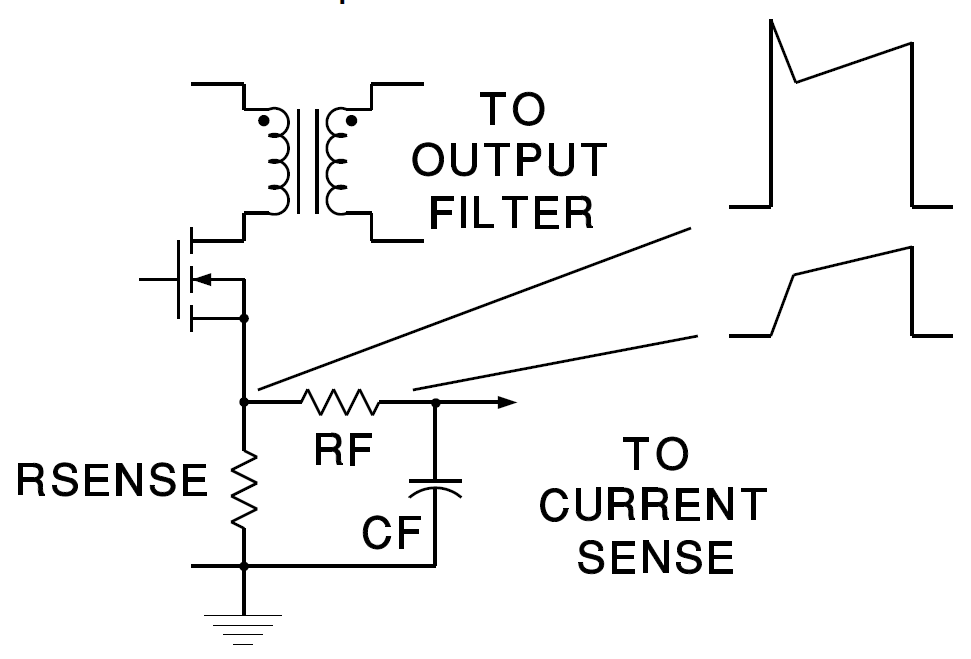
\includegraphics[max width=0.7\linewidth]{/tex/2iteration/billeder/ucc1801_CS_filter.PNG}
	\caption{Current sense signal før og efter eksternt RC-filter}
	\label{fig:ucc1801_CS_filter}
\end{figure}

\subsubsection{Overstrømsbeskyttelse} \label{CS_protection}
En fordel ved, at regulere efter strømmen i transformatoren er, at der opnås en overstrømsbeskyttelse. Når strømmen stiger, vil PWM-controlleren sænke duty-cyclen, og derved også sænke udgangsspændingen. Dette giver en I/V karakteristik der, ideelt set, er næsten firkantet. Dette er skitseret på figur~\ref{fig:I-V_karateristik}. 

\begin{figure}[H]
	\center
	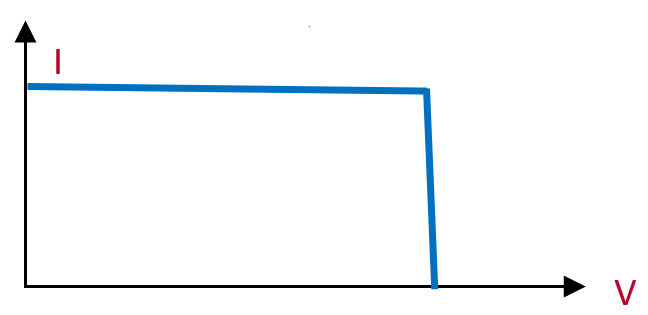
\includegraphics[max width=0.7\linewidth]{/tex/2iteration/billeder/I-V_karakteristik.PNG}
	\caption{I/V karakteristik for converteren}
	\label{fig:I-V_karateristik}
\end{figure}

Denne karakteristik kan dog ikke opnås i realiteten. Filteret der er indsat for at filtrere current sense signalet, vil lave en hale på karakteristikken. Det sker fordi controlleren ikke ser den faktiske strøm, men den filtrerede, når duty-cyclen er lav. 

Da det er nødvendigt at filtrere current sense signalet, men samtidig påvirker converterens I/V karakteristik, optimeres filteret ofte således, det kun akkurat filtrer nok. Denne optimering vil ske i 3. iteration. 

\subsection{Spændingsregulering} \label{V_loop}
I dette afsnit beskrives spændingssløjfen. Den består hovedsageligt af to dele: en spændingsdeler og en fejlforstærker. Spændingsdeleren deler udgangsspændingen ned, så den ønskede udgangsspænding er lig en intern reference i IC'en. Fejlforstærkeren står for selve reguleringen. Den inverterende indgang og udgangen på fejlforstærkeren er ført ud, således det er muligt at indsætte et kompenseringsnetværk.

\subsubsection{Spændingsdeler}
Den ikke inverterende indgang på den indbyggede fejlforstærker i UCC1801, er forbundet til den halve reference spænding, dvs. $2.5V$. Derfor skal der designes en spændingsdeler, der deler den ønskede udgangsspænding på $21V$ ned til $2.5V$. Figur~\ref{fig:Voltagedivider_ideal} viser kredsløbet for spændingsdeleren. 

\begin{figure}[H]
	\center
	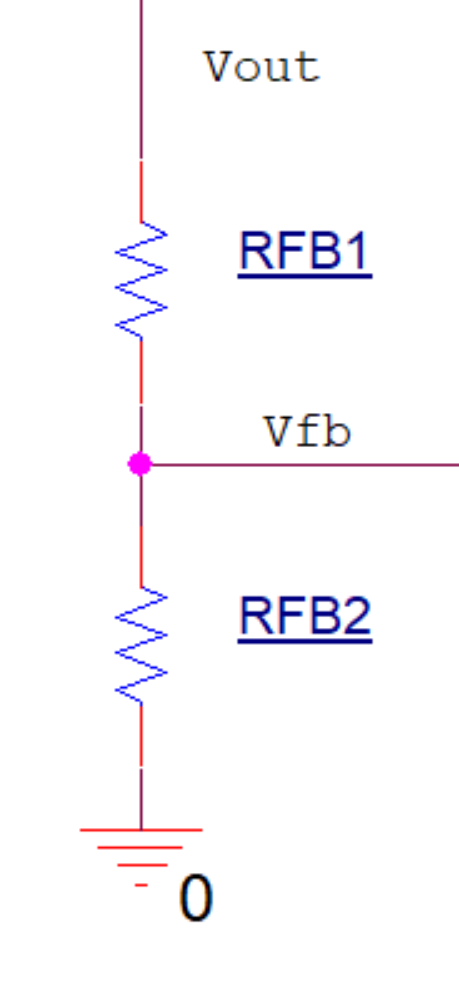
\includegraphics[max width=0.7\linewidth]{/tex/2iteration/billeder/Voltagedivider_ideal.PNG}
	\caption{Spændingsdeler diagram}
	\label{fig:Voltagedivider_ideal}
\end{figure}

Spændingsdeleren designes således der løber en strøm på $1mA$ i den. Derved påvirker den ikke udgangsstrømmen. Derudover dimensioneres de to modstande, således der er et spændingsfald på $2.5V$ over $R_{FB2}$, og $21V-2.5V$ over $R_{FB1}$. $R_{FB1}$ er beregnet med ligning~\ref{RFB1}.

\begin{equation} \label{RFB1}
R_{FB1} = \frac{V_{out}-V_{FB}}{I_{FB1}} = \frac{21V-2.5V}{1mA} = 18.5k\ohm
\end{equation}

\noindent $R_{FB2}$ er beregnet ud fra spændingsdeler formlen, ligning~\ref{RFB2}. Her løses $R_{FB2}$, og fås til $R_{FB2}=2.527k \ohm$.  
\begin{equation} \label{RFB2}
V_{FB} = \frac{R_{FB2}}{R_{FB1} + R_{RB2}} \cdot V_{out}
\end{equation}

For at opnå en præcis spændingsdeler vælges der at bruge to modstande i parallel. Den ene modstand vælges til $R_{FB21}=2.55k\ohm$. Mens den anden regnes ud fra den ønskede samlede modstandsværdi. Dette gøres ved ligning~\ref{RFB22}, som løses med hensyn til $R_{FB22}$. Dette giver $R_{FB22}=280.5k\ohm$, som afrundes til $280k\ohm$.
\begin{equation} \label{RFB22}
R_{FB2} = ((R_{FB21})^{-1} + (R_{FB22})^{-1})^{-1}
\end{equation}

\subsubsection{Fejlforstærker}
Som en del af reguleringen opstilles der først en overføringsfunktion for power-modulet. Denne overføringsfunktion er opgivet i databladet for UCC1801, og er skrevet ved ligning~\ref{H_Power}.
\begin{equation} \label{H_Power}
G_{pwr}(s) = G_0 \cdot \frac{(1+\frac{s}{2\pi \cdot f_{ESRz}}) \cdot (1-\frac{s}{2\pi \cdot f_{RHPz}})}{1+\frac{s}{2\pi \cdot f_{p1}}} \cdot \frac{1}{1 + \frac{s}{2\pi \cdot f_{p2}} + \frac{s^2}{(2\pi \cdot f_{p2})^2}}
\end{equation}

Overføringsfunktionen består af flere dele: en DC-forstærkning, to poler og to nulpunkter. DC-forstærkningen, $G_0$, er skrevet ved ligning~\ref{DC_gain}. Den er især bestemt af belastningen, current sense kredsløbet, transformatoren og switch-frekvensen. Den regnes til en forstærkning på $10.74$ gange, eller $20.6\decibel$.
\begin{equation} \label{DC_gain}
G_0 = \frac{R_{out} \cdot N}{R_{CS} \cdot A_{CS}} \cdot \frac{1}{\frac{(1-D)^2}{\tau_L} + (2 \cdot M) + 1} = 10.7GG \Rightarrow 20.6\decibel
\end{equation}
\noindent Hvor:
\newline \noindent $N$ er omsætningsforholdet i transformatoren.
\newline \noindent $A_{CS}$ er den interne forstærkning i current sense kredsløbet, og aflæses i databladet til $1.65$.
\newline \noindent $D$ er den maksimale duty-cycle, som er $0.447$.
\newline \noindent $\tau_L$ er converterens tidskonstant. Den regnes ud fra ligning~\ref{tau_L}.
\begin{equation} \label{tau_L}
\tau_L = \frac{2 \cdot L_P \cdot f_s}{R_{out} \cdot N^2}
\end{equation}
\newline \noindent $M$ er spændingsomsætningen fra indgang til udgang. Den regnes ud fra ligning~\ref{M}.
\begin{equation} \label{M}
M = \frac{V_{out} \cdot N}{V_{in}}
\end{equation}

En flyback converter, som opererer i CCM, har to primære nulpunkter der kan påvirke stabiliteten i systemet. Det er også de to nulpunkter der er inkluderet i overføringsfunktionen. Den ene, $f_{ESRz}$, er bestemt af produktet mellem udgangskapaciteten og den indre seriemodstand i udgangskondensatoren. Placeringen af denne er regnet ved ligning~\ref{ESR_zero}.
\begin{equation} \label{ESR_zero}
f_{ESRz} = \frac{1}{2 \cdot \pi \cdot R_{ESR} \cdot C_{out}} = 189.5k\hertz
\end{equation}

Det andet nulpunkt er højre-halvplans-nulpunktet. Det er ofte dette nulpunkt der er det dominerende af de to, og derfor den der skal tages højde for i reguleringen. Placeringen af dette er regnet ved ligning~\ref{RHP_zero}. Placeringen af dette nulpunkt, er afhængigt af størrelsen på belastningen, samt inputspændingen. Placeringen stiger ved højere inputspændinger, og mindre belastninger. 
\begin{equation} \label{RHP_zero}
f_{RHPz} = \frac{R_{out} \cdot (1-D)^2 \cdot N^2}{2 \cdot \pi \cdot L_P \cdot D} = 15.8k\hertz
\end{equation}

\noindent Ud fra ligning~\ref{ESR_zero} og \ref{RHP_zero}, ses det, at det er højre-halvplans nulpunktet der er det dominerende nulpunkt i converteren. Når båndbredden skal vælges, er det derfor vigtigt, at den ligger tilpas meget lavere end det dominerende nulpunkt.

Converteren har også to relevante poler. Den dominerende pol bestemmes af load'en og udgangskondensatoren. Den anden pol er placeret ved den halve switching-frekvens. De to poler er beregnet ved ligning~\ref{pol1} og \ref{pol2}.
\begin{equation} \label{pol1}
f_{p1} = \frac{\frac{(1-D)^3}{\tau_L} + 1 + D}{2\cdot \pi \cdot R_{out} \cdot C_{out}} = 132.8\hertz
\end{equation}

\begin{equation} \label{pol2}
f_{p2} = \frac{f_s}{2} = 50k\hertz
\end{equation}

\noindent Bode plottet for power-modulet plottes i MATLAB på figur~\ref{fig:MATLAB_power_module}. Her aflæses DC-forstærkningen til $20.6\decibel$. Derudover aflæses der en pol ved ca. $130\hertz$ og ved ca. $50k\hertz$. Dette stemmer overens med de beregnede værdier.

Konsekvensen af højre-halvplans nulpunktet ses også tydeligt på figur~\ref{fig:MATLAB_power_module}. Når frekvensen nærmer sig nulpunktet bliver forstærkningen øget med $20 \decibel$/decade, som ved et venstre-halvplans nulpunkt. Tilgengæld vil fasen blive trukket ned med $90^\circ$, i stedet for op. Da polen fra switch-frekvensen ligger ca. samme sted, og også trækker fasen ned med $90^\circ$, kommer der et stort fasedrej i dette frekvensområde. Det kan gøre systemet ustabilt hvis gain-marginen ikke er tilstrækkelig stor. 

\begin{figure}[H]
	\center
	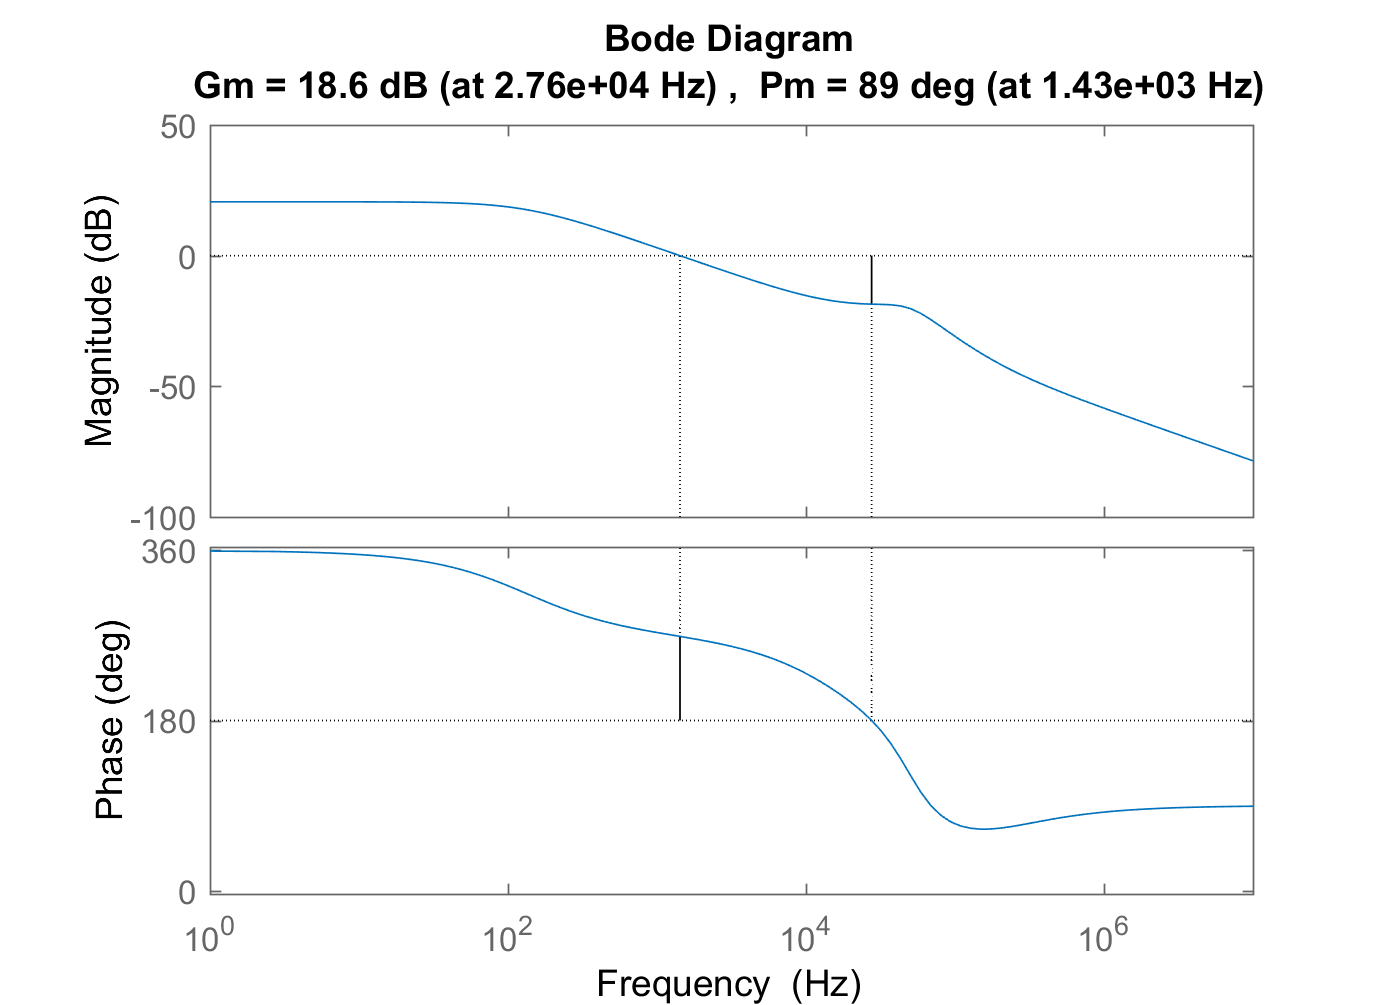
\includegraphics[max width=0.7\linewidth]{/tex/2iteration/billeder/MATLAB_power_module.PNG}
	\caption{Bode plot for power-modulet}
	\label{fig:MATLAB_power_module}
\end{figure}

I denne iteration designes der et kompensationsnetværk der vil sikre et stabilt system, med en lav båndbredde. Dette vil blive optimeret i en senere iteration. 
Da der ønskes en lavere båndbredde, end det converteren har i forvejen, indsættes et RC-led i serie som kompensationsnetværk. Ved at bruge et RC-led, vil kondensatoren bestemme forstærkningen ved lave frekvenser, fordi impedansen her er stor. Mens modstanden vil bestemme forstærkningen ved høje frekvenser, fordi kondensatoren vil blive set som en kortslutning. 

Den endelige båndbredde af systemet ønskes på ca. $800\hertz$. Det vil sikre, at systemet ikke bliver ustabilt. For at opnå den ønskede båndbredde aflæses det ud fra bode plottet på figur~\ref{fig:MATLAB_power_module}, at forstærkningen skal mindskes med ca. $5.4\decibel$, eller ca. $0.535GG$, ved frekvenser over $800\hertz$. Den samlede forstærkning af reguleringssløjfen, bestemmes af produktet mellem forstærkningen i spændingsdeleren og forstærkningen i fejlforstærkeren. Forstærkningen i spændingsdeleren regnes ved ligning~\ref{voltagedivider_gain}.
\begin{equation} \label{voltagedivider_gain}
g_{FB} = \frac{R_{FB2}}{R_{FB1}+R_{FB2}} = 0.12
\end{equation}

\noindent Nu kan feedback modstanden i fejlforstærkeren regnes ved ligning~\ref{error_opamp_gain}. 
\begin{equation} \label{error_opamp_gain}
g_{tot} = \frac{R_{comp}}{R_{par}} \cdot g_{FB}
\end{equation}

\noindent Hvor:
\newline \noindent $g_{tot}$ er det ønskede gain i fejlforstærkeren, som er $g_{tot}=0.535GG$.
\newline \noindent $R_{comp}$ er feedback modstanden i fejlforstærkeren, som ønskes dimensioneret.
\newline \noindent $R_{par}$ er parallelmodstanden mellem $R_{FB1}$ og $R_{FB2}$. Den regnes til $R_{par}=2.244k\ohm$.

\noindent De kendte værdier indsættes og ligningen løses for $R_{comp}$. Den fås til $R_{comp}\approx 10k\ohm$.


\noindent For at sikre en den lave båndbredde, sættes knækfrekvensen på integratoren til $f_0=300\hertz$. Dermed sikres det, at fejlforstærkeren dæmper signalet ved den ønskede båndbredde på $800\hertz$. Nu den tilhørende kapacitet regnes, ud fra $R_{comp}$ og $f_0$.
\begin{equation} \label{c_comp}
c_{comp} = \frac{1}{2\cdot \pi \cdot R_{comp} \cdot f_0} \approx 50nF
\end{equation}

\noindent Med afrundede komponentværdier, regnes den nye knækfrekvens for fejlforstærkeren.
\begin{equation} \label{f_0}
f_0 = \frac{1}{2\cdot \pi \cdot R_{comp}} \cdot c_{comp} = 318.3\hertz
\end{equation}

\noindent Overføringsfunktionen for fejlforstærkeren kan nu opskrives ved ligning~\ref{H_err}.
\begin{equation} \label{H_err}
G_{err}(s) = (\frac{318.3\hertz \cdot 2\cdot\pi}{s} + 1) \cdot 0.535
\end{equation}

\noindent Den plottes i MATLAB, som et bode plot på figur~\ref{fig:MATLAB_error_op_amp_2}. Her ses det, at den ønskede funktion af integratoren er opnået. På grund af kondensatoren, har den et stort gain ved lave frekvenser. Mens forstærkningen ligger konstant ved ca. $-5.4\decibel$, efter den ønskede knækfrekvens på ca. $318\hertz$.

\begin{figure}[H]
	\center
	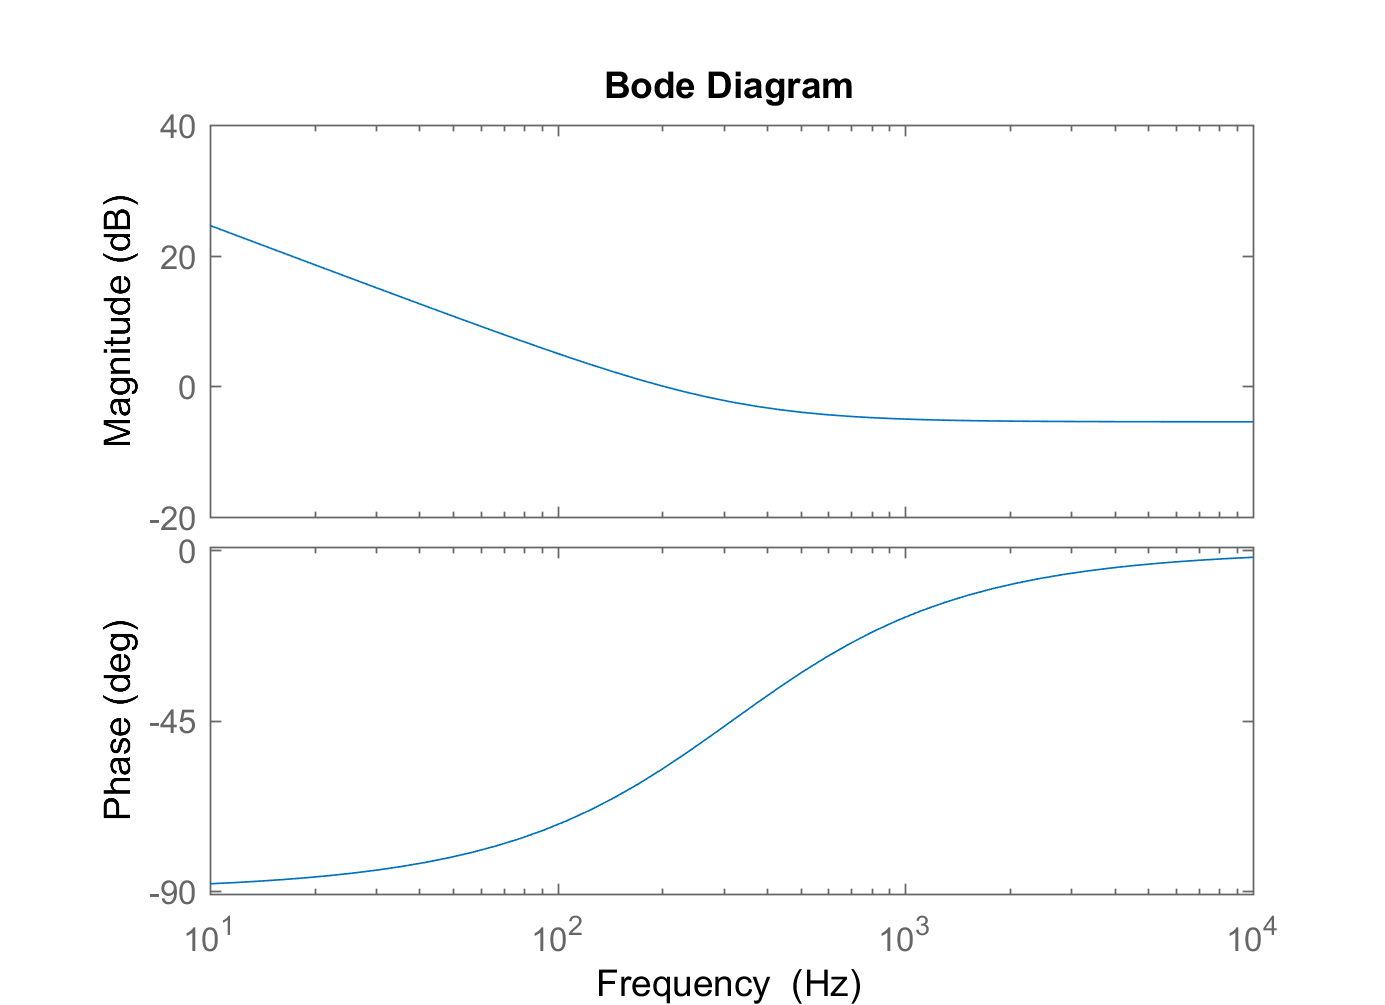
\includegraphics[max width=0.7\linewidth]{/tex/2iteration/billeder/MATLAB_error_op_amp.PNG}
	\caption{Bode plot for fejlforstærker}
	\label{fig:MATLAB_error_op_amp_2}
\end{figure}

De to overføringsfunktioner ganges sammen for, at bestemme den samlede overføringsfunktion for converteren. Figur~\ref{fig:MATLAB_total_2} viser et åben sløjfe bode plot af det. Det aflæses at converteren vil have en båndbredde på $810\hertz$. Derudover aflæses fase-margin til $74.3^\circ$, og gain-margin til $24\decibel$.

\begin{figure}[H]
	\center
	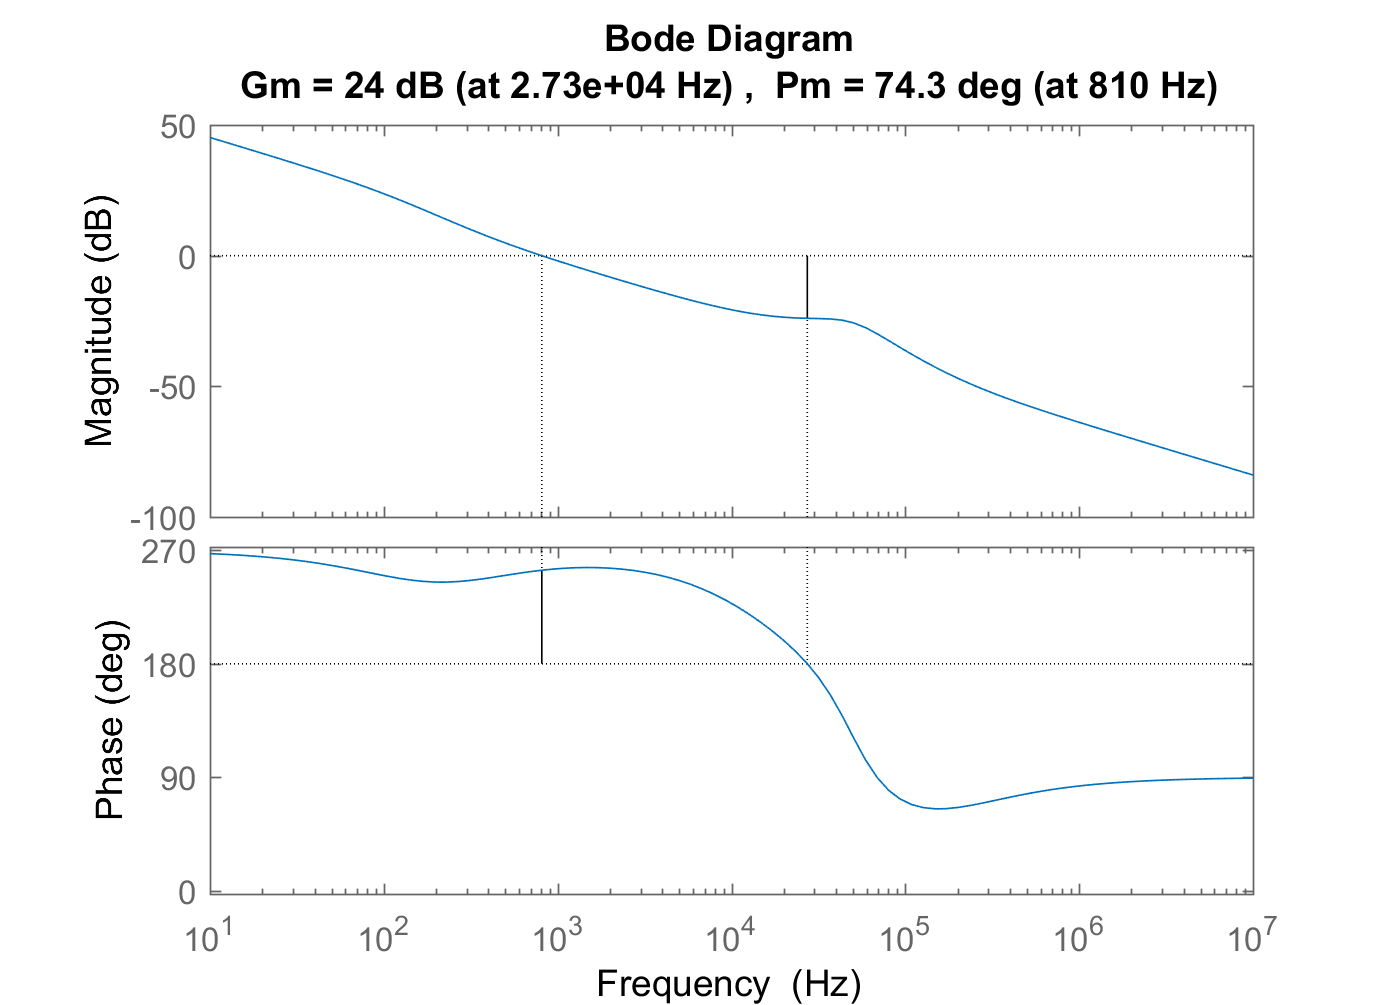
\includegraphics[max width=0.7\linewidth]{/tex/2iteration/billeder/MATLAB_total.PNG}
	\caption{Bode plot for converteren}
	\label{fig:MATLAB_total_2}
\end{figure} 



<<<<<<< HEAD
=======

\section{Diode}
For at mindske tabet i konverteren skal spændingsfaldet over dioden helst være så lille som muligt. Der skal dog sørges for, at dioden kan holde til den spænding, der ligger over den, når transistoren er on. Denne breakdown voltage er den maksimale indgangsspændingen plus udgangsspændingen. Faktoren på $1.3$, der ganges på, er en sikkerhedsmargin på $30\percent$:
\begin{equation} \label{Vd_break}
Vd_{break} = (V_{out}+V_{inmax}) \cdot 1.3 = 92.3V
\end{equation}
Yderligere skal dioden kunne holde til RMS strømmen på udgangen på de $3.36A$ og en peakstrøm på $5.53A$.
Schottky dioden NTSV30120CT er valgt til 2. iteration med en breakdown voltage på $120V$. Dioden kan klare en continuos strøm $5A$ og en peakstrøm på $30A$ per device. Hele devicet er med 2 dioder, og da der her kun benyttes én af dem, er det i stedet en peakstrøm på $15A$, der er maksimum. Derudover kan dens spændingsfald aflæses i databladet til ca. $0.5V$ ved $125\degreeCelsius$ og $3.36A$. 
>>>>>>> c2a744e3a54742ae7689fa63cbb3692dd6281371

\section{MOSFET} \label{MOSFET}
MOSFET'en skal først og fremmest kunne holde til den spænding, der vil ligge over drain-source, når den er off. Ved en flyback er det den maksimale indgangsspænding plus den spænding der bliver reflekteret tilbage til primærviklingen fra sekundærviklingen. Det vil sige udgangsspændingen samt diodens spændingsfald. Det vil ideelt set betyde, at MOSFET'en skal kunne holde til:
\begin{equation} \label{Vds_breakideel}
Vds_{breakideel} = (V_{inmax}+(V_{out}+V_D))= 71.5
\end{equation}
Der bør istedet ganges en sikkerhedsmargin oveni på $30\percent$. Det er til for at tage højde for de peakspændinger, der vil komme når der switches. De skyldes kombinationen af spredningsselvinduktionen og kapaciteterne fra MOSFET og diode. Derudover vil der også være kapacitet grundet transformatorens kobling. Typisk vil MOSFET og diodens kapaciteter være større og dermed dominerende. Tages der højde for disse spændingstransienter skal MOSFET'en minimum kunne holde til en spænding på: 
\begin{equation} \label{Vds_break}
Vds_{break} = (V_{inmax}+(V_{out}+V_D)) \cdot 1.3 = 92.95
\end{equation}
Yderligere skal den valgte MOSFET kunne holde til RMS strømmen i primærviklingen på $3.02A$ samt peakstrømmen på $5.64A$.
Til 2. iteration er IRFB23N15 valgt.(datasheet henvisning) Den kan holde til Vds på $150V$ og en continous drain strøm på $17A$ samt en peak på $92A$, hvilket er rigeligt. Derudover en Rds(on) modstand på ca. $113\milli \ohm$ ved $50\degreeCelsius$. 

Det er en MOSFET, som vil kunne fungere i designet, men som også kan optimeres på on modstand og kapacitet på et senere tidspunkt, hvis tabet ender med at være for stort. 

\section{Diode}
For at mindske tabet i konverteren skal spændingsfaldet over dioden helst være så lille som muligt. Der skal dog sørges for, at dioden kan holde til den spænding, der ligger over den, når transistoren er on. Denne breakdown voltage er ideelt se den maksimale indgangsspændingen plus udgangsspændingen.
\begin{equation} \label{Vd_breakideel}
Vd_{breakideel} = (V_{out}+V_{inmax}) = 71V
\end{equation}
Igen skal der i realiteten tages højde for peakspændinger ligesom ved MOSFET'en. Der ganges derfor igen en faktor 1.3 på, og dioden skal dermed kunne holde til spændingen:
\begin{equation} \label{Vd_break}
Vd_{break} = (V_{out}+V_{inmax}) \cdot 1.3 = 92.3V
\end{equation}
Yderligere skal dioden kunne holde til RMS strømmen på udgangen på de $3.36A$ og en peakstrøm på $5.53A$.
Schottky dioden NTSV30120CT er valgt til 2. iteration med en breakdown voltage på $120V$. Dioden kan klare en continuos strøm $5A$ og en peakstrøm på $30A$ per device. Hele devicet er med 2 dioder, og da der her kun benyttes én af dem, er det i stedet en peakstrøm på $15A$, der er maksimum. Derudover kan dens spændingsfald aflæses i databladet til ca. $0.45V$ ved $125\degreeCelsius$ og $2.5A$. 

\section{Udgangskondensator}
Som udgangskondensator er valget faldet på 4 parallelle kondensatorer på $56\micro F$ af typen .. Dette var den film kondensator med højest kapacitet Terma havde til rådighed. Det vigtige her, er at det er en film kondensator, da de typisk har ret præcise kapaciteter samt en lav ESR modstand. Når kondensatorer ikke længere anses som ideele, vil der i virkeligheden både være en ESL induktans og en ESR modstand. Ækvivalentdiagrammet for en kondensator vil derfor se ud som på figur~\ref{fig: con_equi} 
\begin{figure}[H]
	\center
	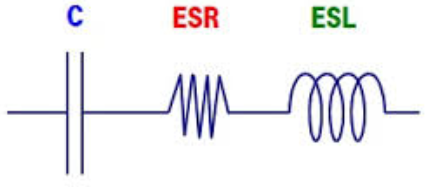
\includegraphics[max width=0.7\linewidth]{/tex/2iteration/billeder/Kondensator_equivalent.png}
	\caption{Ækvivalentdiagram for kondensatorer}
	\label{fig: con_equi}
\end{figure}
I nogle datablade kan disse parasitkomponenter slås op, det er dog ikke tilfældet for denne kondensator. Med hensyn til ESR modstanden, bliver denne af og til ikke oplyst for film kondensatorer, da den er lav ved denne type, i forhold til for eksempel en elektrolyt. 
Med hensyn til induktansen kan den estimeres ved en hovedregel, der siger, $1\nano H$ per $\milli m$. Denne kondensator har $4\centi m$ lang og induktansen estimeres dermed til $40\nano F$. Med 4 kondensatorer i parrallel giver det dermed en samlet induktans for udgangskondensatoren på:
\begin{equation} \label{ESL}
C_{ESL} = ((40\nano F)^{-1} \cdot 4)^{-1} = 10\nano F
\end{equation}

\subsection{Test af kondensator}

For at få ESR modstanden og den præcise ESL induktans, måles disse med impedansmåleren, som også blev benyttet til måling af transformatoren. Opstillingen ses på figur~\ref{fig: cap}, men er den samme som tidligere, hvor transformatoren er skiftet ud med en af kondensatorerne. 
\begin{figure}[H]
	\center
	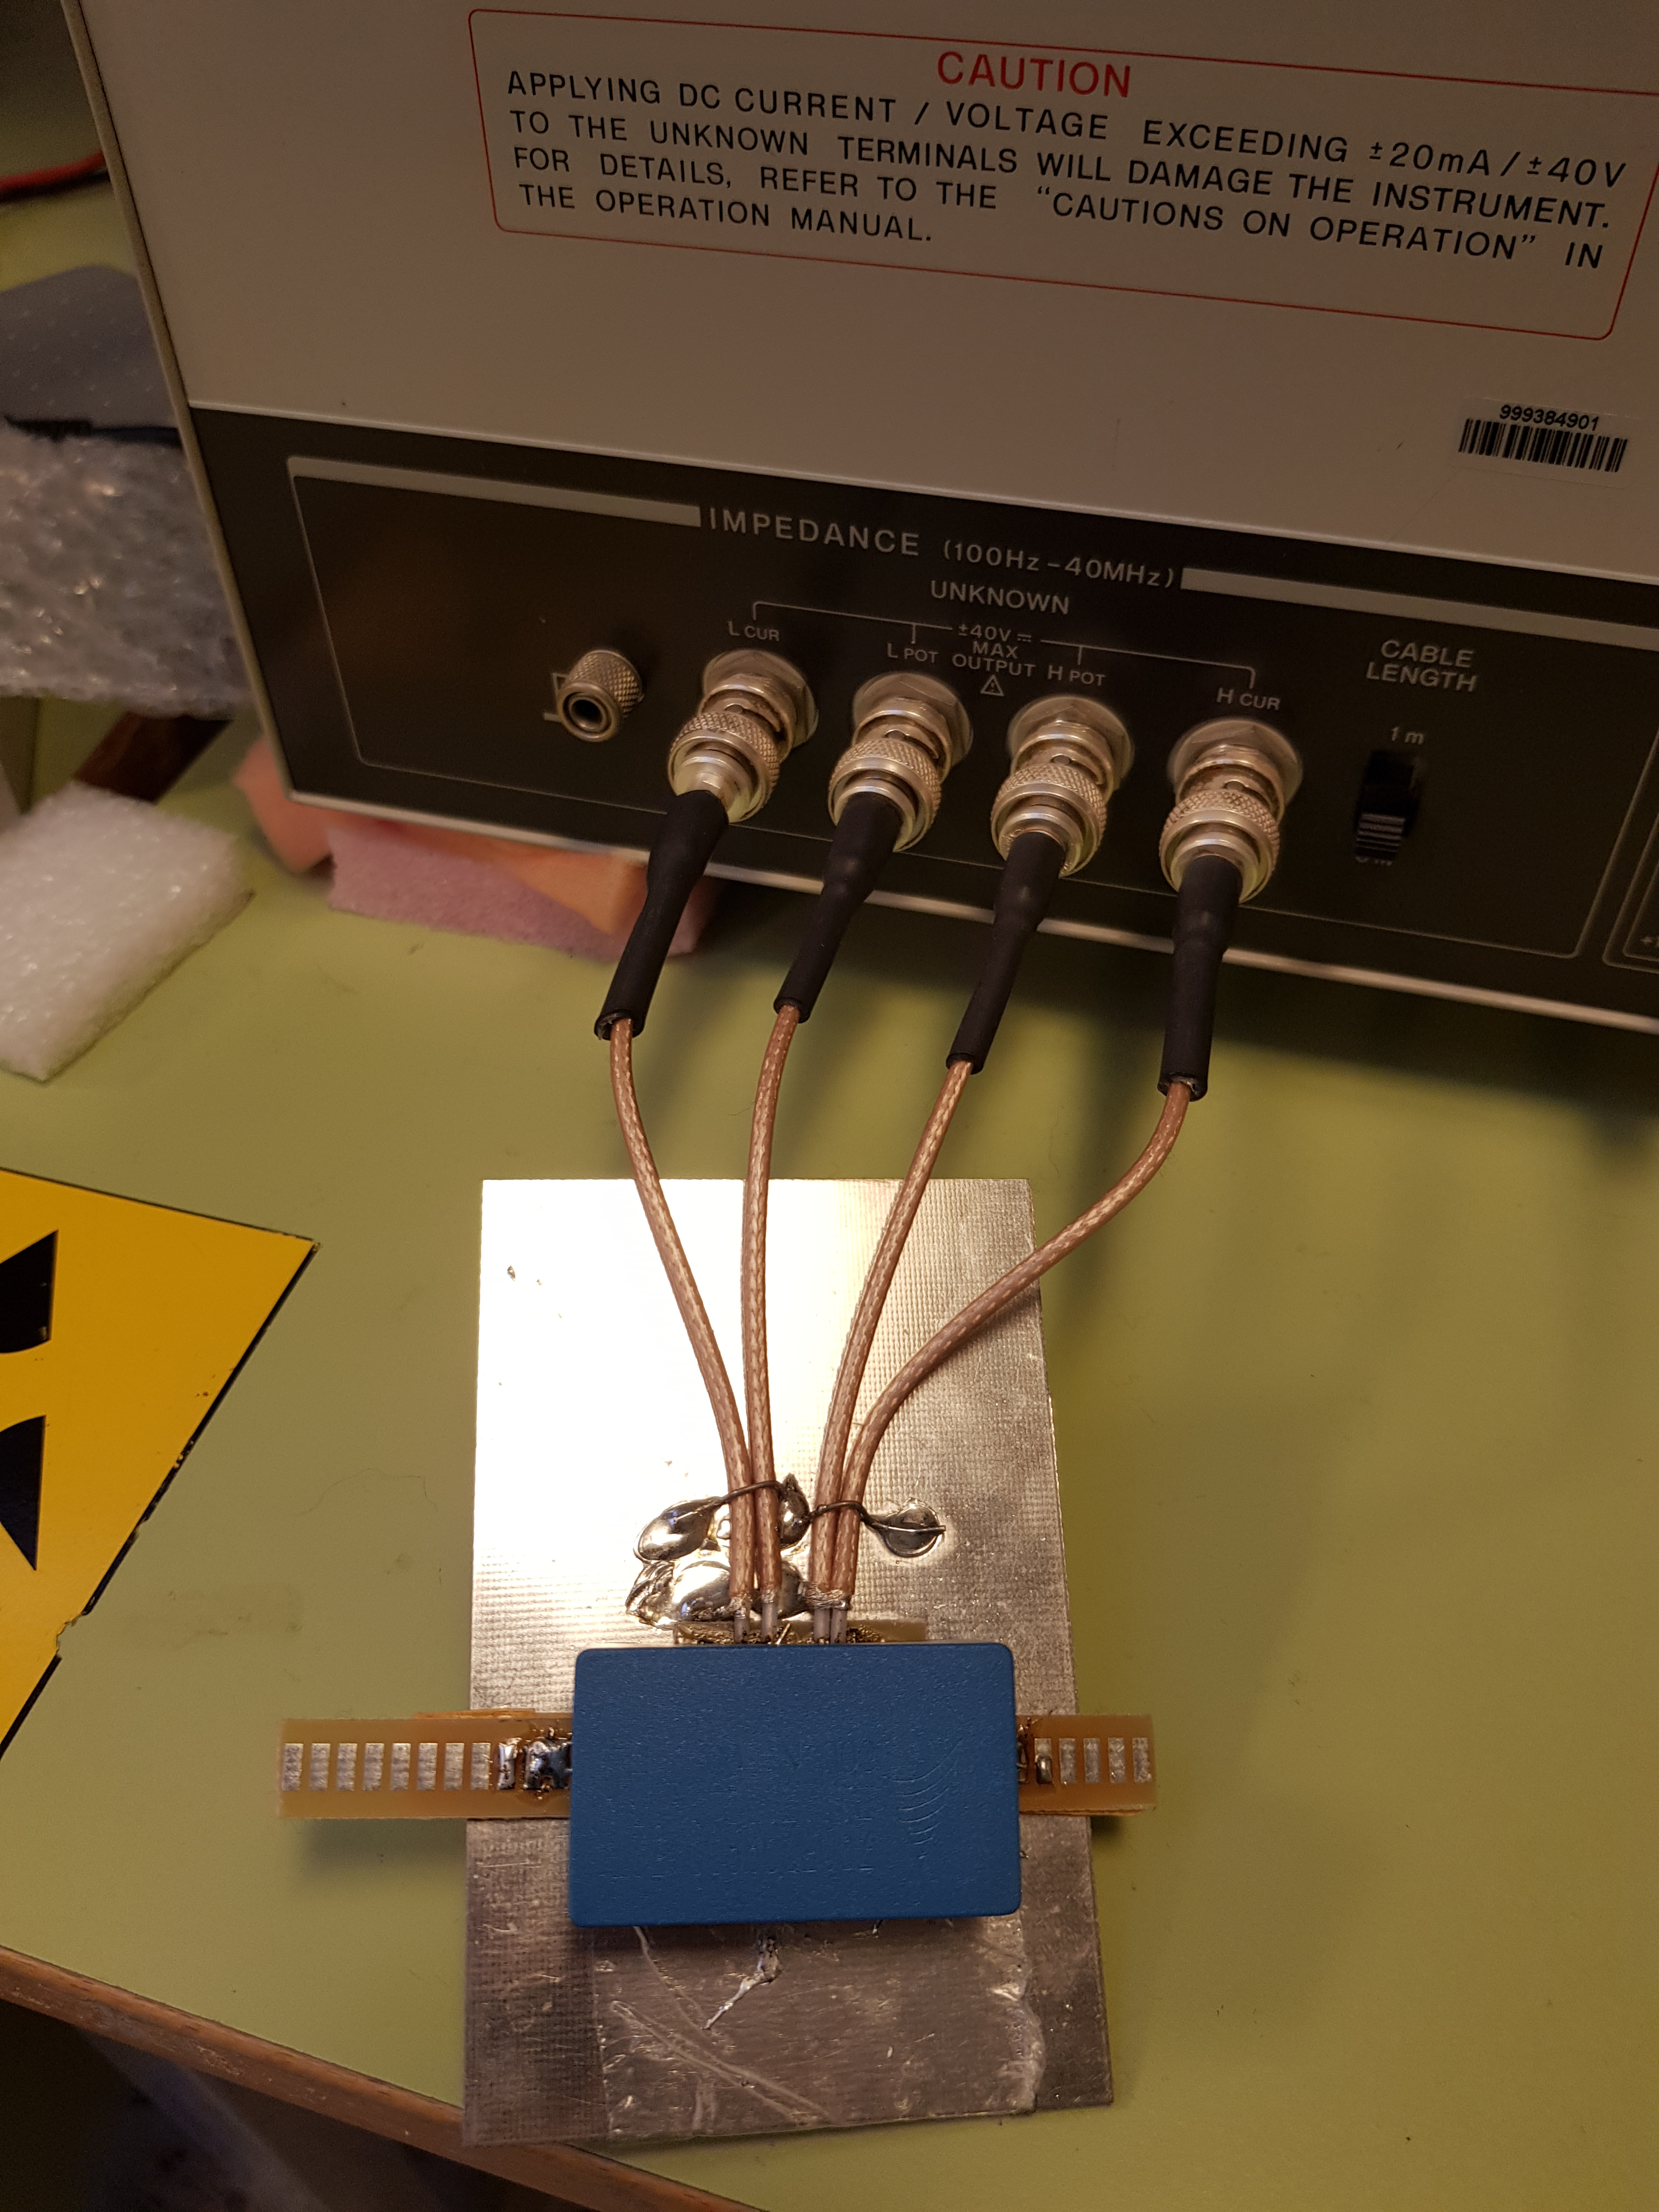
\includegraphics[max width=0.7\linewidth]{/tex/2iteration/billeder/Udgangskondensator_impedansmaling.jpg}
	\caption{Test af udgangskondensator}
	\label{fig: cap}
\end{figure}
Ligesom ved transformatoren benyttes 4-wire teknikken, for at undgå ekstra parasitter. På figur~\ref{fig: captest} ses grafen der er tegnet ud fra målingen. De enkelte målepunkter kan findes i Excel dokumentet \cite{Kondensator_impedans.xlsx}
\begin{figure}[H]
	\center
	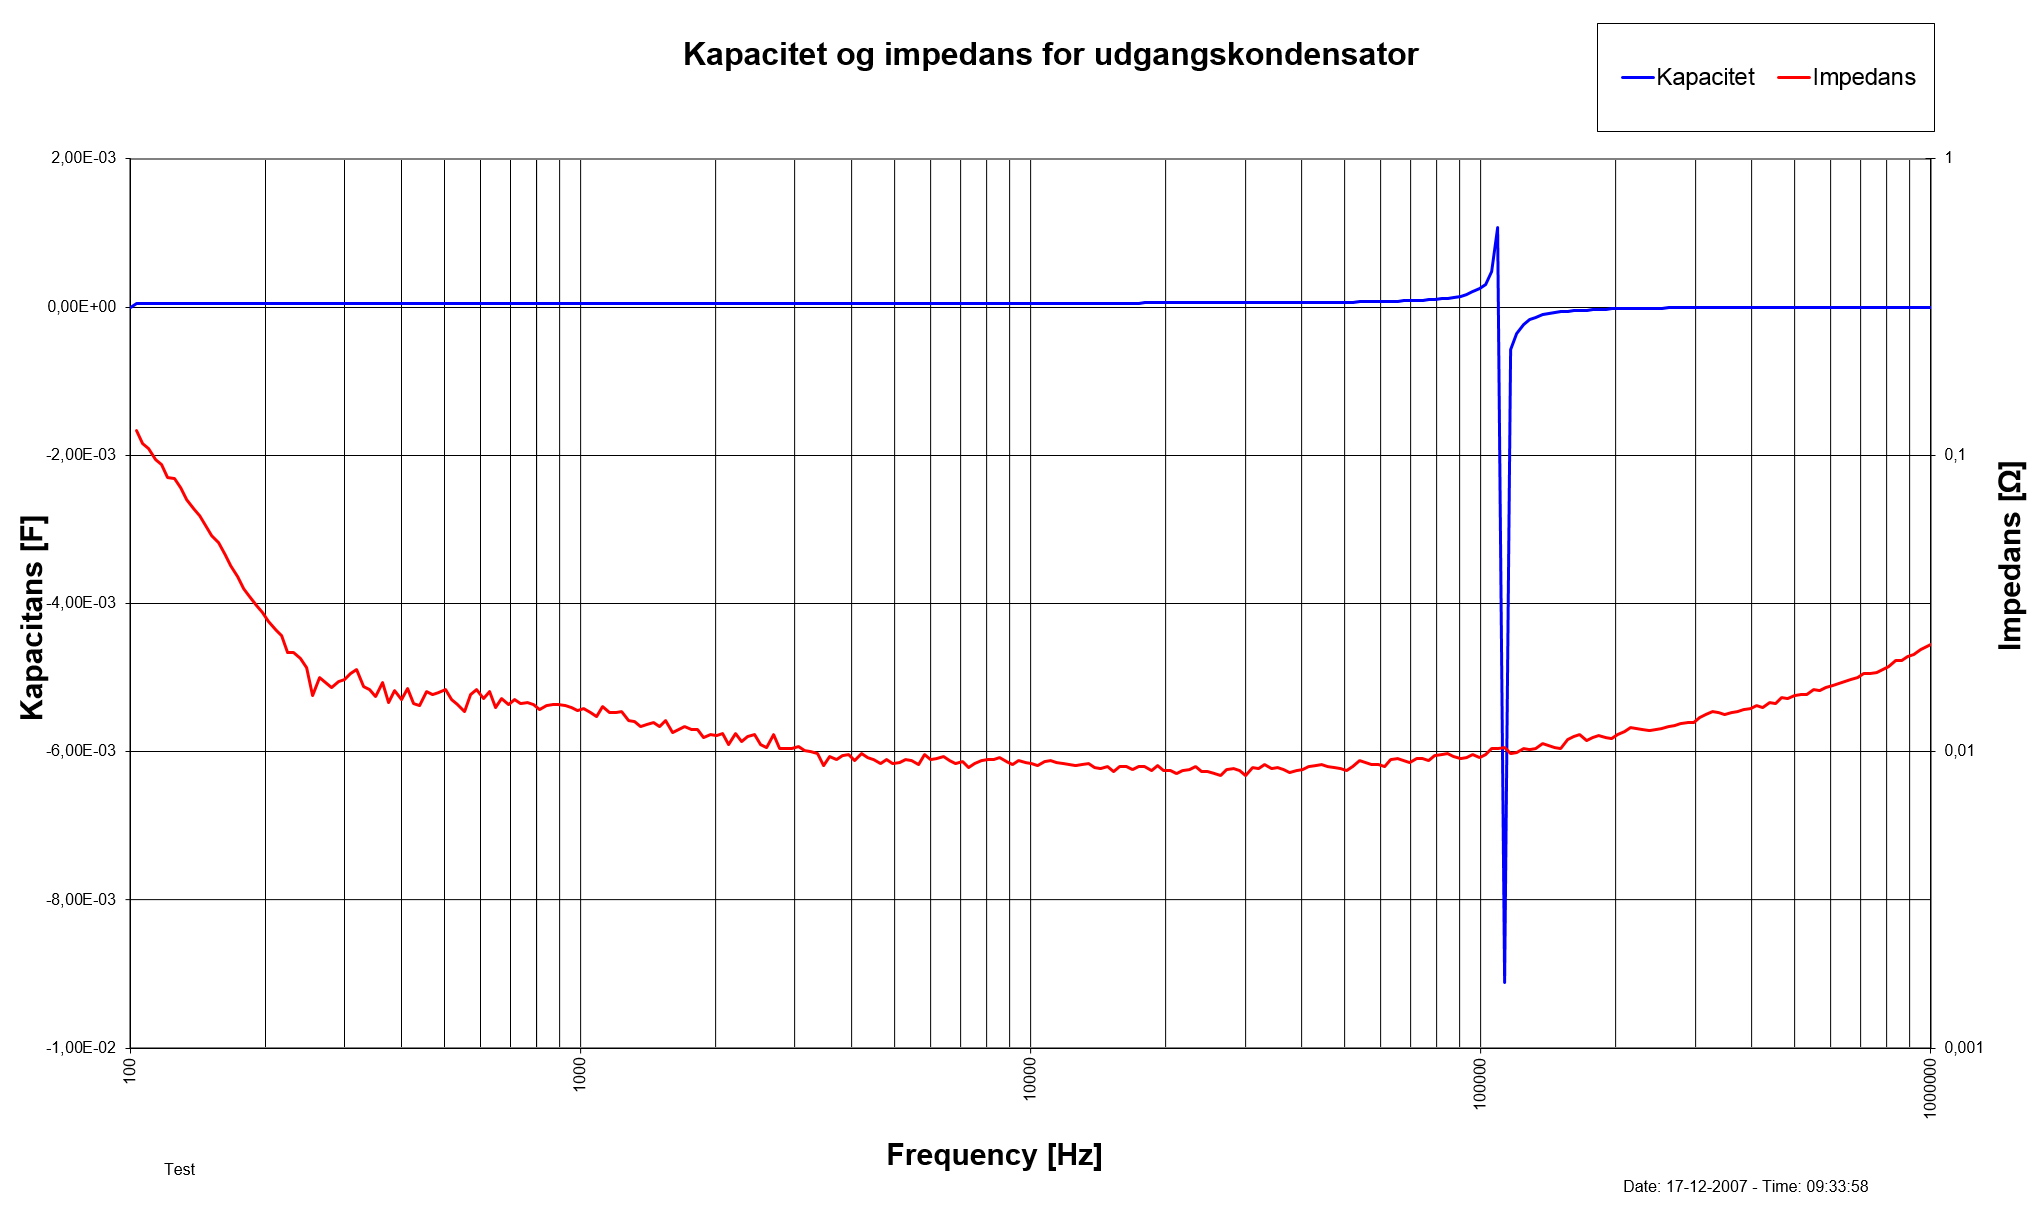
\includegraphics[max width=0.9\linewidth]{/tex/2iteration/billeder/Kondensatortest.png}
	\caption{Kapacitet og impedans for udgangskondensator}
	\label{fig: captest}
\end{figure}
Det ses tydeligt at resonantfrekvensen for det induktive og kapacitive i kondensatoren ligger lidt over de $100\kilo \hertz$, mere præcis ved $108\kilo \hertz$. 


\noindent Da der i projektet bruges en switchfrekvens på $100\kilo \hertz$, er en resonantfrekvens på $108\kilo \hertz$ ikke helt optimal. Det betyder, at der ved de $100\kilo \hertz$, formodentligt ikke vil være præcis den kapacitet der forventes. Det er dog stadig denne kondensator, der benyttes i 2. iteration. Skal der senere optimeres på dette, kan resonantfrekvensen rykkes længere op i frekvens. Det kan enten gøres ved at finde en lignende kondensator med mindre ESL induktans eller finde en kondensator med lavere kapacitet og sætte flere i parrallel end de nuværende 4.


\noindent Ved resonantfrekvensen kan ESR modstanden nogenlunde aflæses, da det kapacitive og induktive her udligner hinanden. Det vil sige, at kun ESR modstanden står tilbage, hvilket i dette tilfælde aflæses til ca. $10\milli \ohm$. 
ESL modstanden kan udregnes ud fra resonantfrekvensen og kapaciteten på de $56\micro F$:
\begin{equation} \label{CESL}
C_{ESL} = \frac{1}{4 \cdot \pi^{2} \cdot {f_{res}}^{2} \cdot C_{out}} = 38.78\nano H
\end{equation}
Hvilket stemmer meget godt overens med det estimerede på de $40\nano F$.
Det betyder, at der med de 4 kondensatorer i parallel vil være en samlet ESL induktans på: 
\begin{equation} \label{CESLtot}
C_{ESLtot} = ((38.78\nano F)^{-1} \cdot 4)^{-1} = 9.70\nano F
\end{equation}
Samt en samlet ESR modstand på:
\begin{equation} \label{CSRtot}
C_{ESRtot} = ((10\milli \ohm)^{-1} \cdot 4)^{-1} = 2.5\milli \ohm
\end{equation}

\section{Input filter}
Input filtreret har som sådan ikke været en del af projektet, da det er blevet givet af Terma. Dette blev gjort, så der kunne fokuseres andetsteds. 

\noindent Herunder beskrives filtret dog stadig, så der gives forståelse for, hvordan det er designet og hvad det bruges til.

\noindent \cite{Inputfilter} Et input filter er nødvendigt i switch mode power supplies. For det første skal det sikre imod den elektromagnetiske interferens, der bliver genereret fra switching. Hvis denne interferens får lov at komme ud på forsyningsnetværket, vil det påvirke andet udstyr, hvilket selvfølgelig ikke er hensigtsmæssigt. Mængden af  tilladeligt EMI (elektromagnetisk interferens) er fastlagt af standarder verden over, så hvis ikke produktet overholder dette, kommer det aldrig på markedet.

\noindent Udover EMI skal filtret også sikre, at højfrekvent spænding fra forsyningsnettet, ikke når outputtet for power supplien.\fxnote{Converteren?} 

Det er i dette projekt gjort med et parallel dæmpet filter. Det består af et LC led, der giver en overordnet resonant frekvens. I sig selv, bør det kunne sikre sig imod de 2 punkter beskrevet ovenfor. Problemet i kun at bruge denne del, ligger ved knækfrekvensen\fxnote{Find en graf for et anden ordensfilter}. Når filtret er udæmpet, som det er ved et LC, kan der komme stor forstærkning ved cut off frekvensen, og derfor forstærke støjen ved den frekvens istedet. Det betyder at der gerne skal ligge en stor dæmpning ved frekvensen. Med en lille dæmpningsfaktor fås et stort gain ved cut off frekvensen og omvendt. En dårlig dæmpningsfaktor kan give resten af systemet en dårligere performance. Det kan gå ind og påvirke overføringsfunktionen til reguleringsloopet og på den måde få systemet til at oscillere. Hvis der sørges for, at udgangsimpedans kurven for input filtret ligger meget under impedanskurven for konverteren, vil konverterens loop gain ikke blive ændret det store. Det vil sige, at det er vigtigt at holde peak impedansen nede for filtret, for at undgå oscillerings problemer forårsaget af inputfiltret.     

Det er her, det parallelle led kommer ind i billedet. Det består af en modstand i serie med en kondensator. Meningen med modstanden er, at reducere udgangs peak impedancen af filtrets cutoff frekvens. Samtidig vil kondensatoren i serie med modstanden sørge for, at blokere DC delen af inputspændingen og derfor mindske effekttabet i modstanden. Denne kondensator skal have en mindre impedans end modstanden ved resonantfrekvensen og en større kapacitans end filter kapaciteten. Dette vil gøre, at cutoff frekvensen af R-L filtret ikke påvirkes af kondensatoren. På figur~\ref{fig: Inputfilter} ses hele filtret givet af Terma.    
\begin{figure}[H]
	\center
	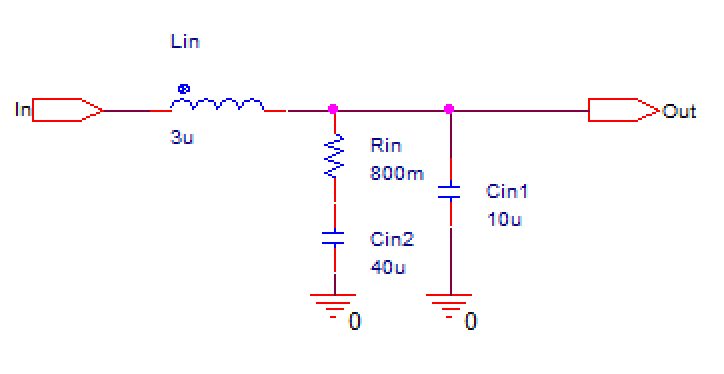
\includegraphics[max width=0.7\linewidth]{/tex/2iteration/billeder/Inputfilter.png}
	\caption{Inputfilter}
	\label{fig: Inputfilter}
\end{figure}
Det ses, at filtret har en overordnet knækfrekvens på:
\begin{equation} \label{fc}
f_c = \frac{1}{2 \cdot \pi \cdot \sqrt{3\micro H \cdot 10\micro F}} = 29.06kHz
\end{equation}
Samtidig kan det konkluderes, at selve kapaciteten på $C_{in2}$ er 4 gange større end $C_{in}$ samt impedansen bliver:
\begin{equation} \label{XC2}
X_{Cin2} = \frac{1}{2 \cdot \pi \cdot 40\micro F \cdot 29.06kHz} = 0.137\ohm
\end{equation}
Hvilket er mindre end modstanden på $0.8\ohm$. Det vil sige, at filtret opfylder kriterier opstillet ovenfor.

\section{Tab}
Her vil tabene for komponenterne i 2. iteration blive udregnet. 

\subsection{Transformatortab}
Transformatortabet kan deles op i 2 dele. Et kernetab og et kobbertab. Det beregnes herunder

\subsubsection{Kernetab}
Selve kernetabet afhænger af kernematerialet, induktans og strømmen der løber i viklingerne. Først udregnes delta B.
\begin{equation} \label{DeltaB}
\Delta B = \frac{L \cdot I_{pk21}}{N \cdot A_0} = 263.59\milli T
\end{equation}
For at få peak fluxen divideres med 2. Med den kan tabet i kernen per $\frac{\kilo W}{m^3}$
\begin{equation} \label{B}
B = \frac{\Delta B}{2} = 131.79\milli T
\end{equation}
Med den information kigges i databladet under kurven for power loss som funktion af peak flux density.
\begin{figure}[H]
	\center
	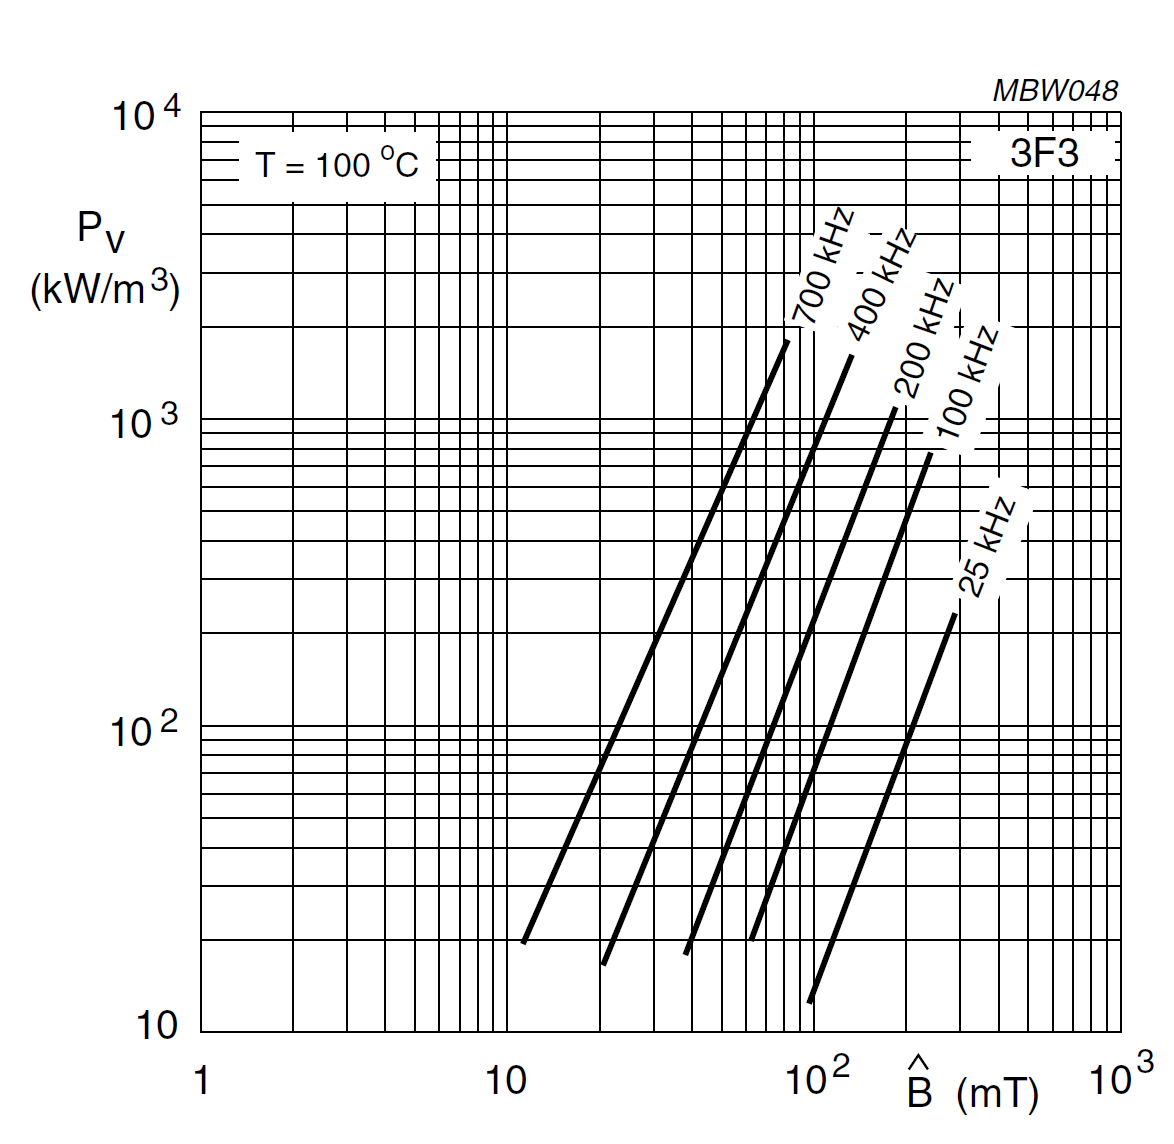
\includegraphics[max width=0.7\linewidth]{/tex/2iteration/billeder/Powerloss.png}
	\caption{Power loss som funktion af peak flux density}
	\label{fig: Powerloss}
\end{figure}
Her ses på de $100\kilo Hz$ ved de ca. $132\milli T$. Det aflæses til et power loss på ca. $150\frac{\kilo W}{m^3}$.
Det samlede kernetab fås med denne værdi ganget med den effektive volumen for RM8 kernen.
\begin{equation} \label{DeltaB}
P = P_V \cdot V_e = 366\milli W
\end{equation}
Dette passer forholdsvis pænt med det simulerede tab i kernen på $310\milli W$.

\subsubsection{Kobbertab}
Kobbertabet i transformatoren opstår på grund af modstanden i de kobbertråde den er viklet med. Den modstand deles op i to bidrag - en DC-modstand og en AC-modstand. DC-modstanden bestemmes ud fra længden og tykkelsen af tråden, mens AC-modstanden afhænger af indtrængningsdybden og trådens diameter. 

\paragraph{AC-modstand}
AC-modstanden i viklingerne opstår på grund af, det magnetfelt kobbertrådene ligger i. Magnetfeltet skaber en hvirvelstrøm der løber i trådene. Hvirvelstrømmen vil derfor være et ekstra bidrag, til den driftsstrøm der bliver sendt ind i transformatoren. Dette vil komme til udtryk, som et ekstra bidrag til den samlede modstand i viklingerne. 

AC-modstanden afhænger af indtrængningsdybden og trådens diameter. Hvis diameteren er tilpas lille i forhold til indtrængningsdybden, vil  hvirvelstrømmene i tråden udligne sig selv, og derved ikke bidrage til tabet. Er tråden til gengæld for tyk i forhold til indtrængningsdybden, vil det resultere i en hvirvelstrøm, der løber i hele trådens længde. 

Måden AC-modstanden bestemmes, er vha. princippet \textit{Eddy Current Losses}. Det siger at forholdet mellem AC- og DC-modstanden, kan bestemmes ud fra forholdet mellem trådens diameter og indtrængningsdybden. Disse forhold er skitseret på figur~\ref{fig:Eddy_current_losses}\cite{eddyCurrentLosses}. Her ses det også, at AC-modstanden afhænger af hvor mange lag der er vikler på transformatoren. 

\begin{figure}[H]
	\center
	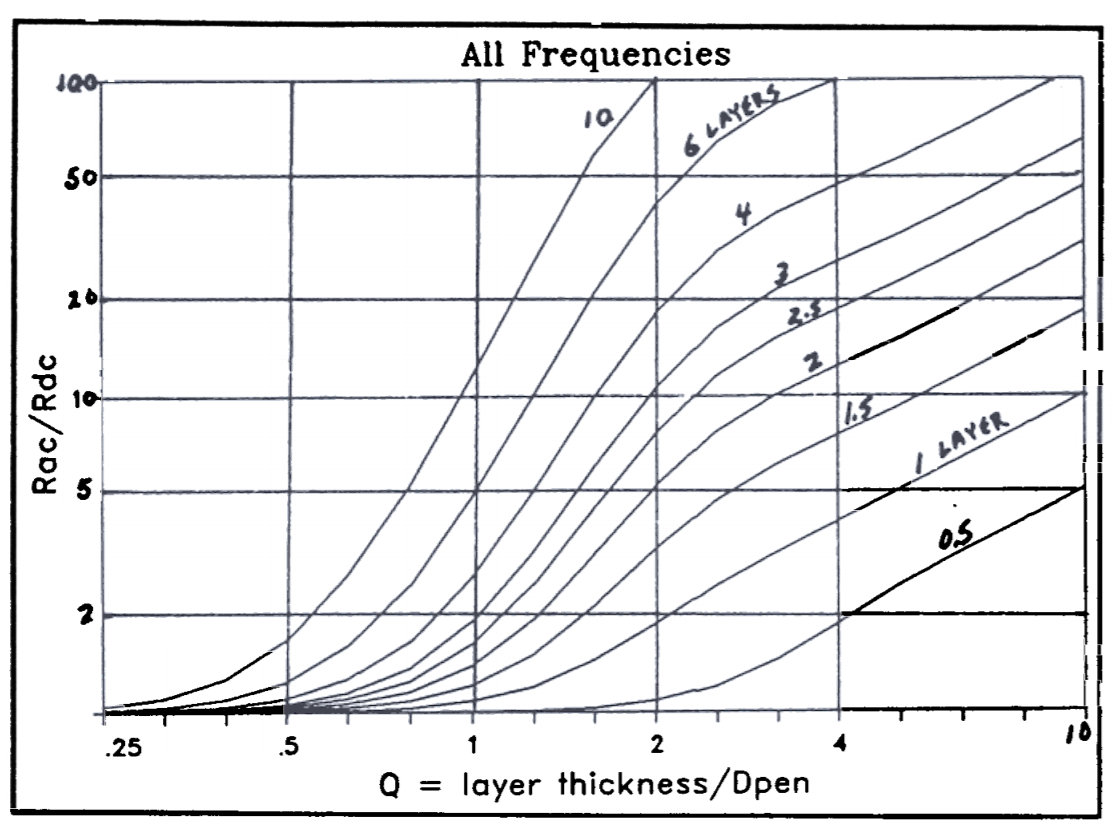
\includegraphics[max width=0.7\linewidth]{/tex/2iteration/billeder/Eddy_current_losses.PNG}
	\caption{Eddy Current Losses}
	\label{fig:Eddy_current_losses}
\end{figure}

Det er valgt at se bort fra AC-modstanden, når kobbertabet regnes. Derfor vil det, kun være en estimering af det samlede kobbertab i transformatoren. 

\paragraph{DC-modstand}
For at beregne DC-modstanden, udregnes først omkredsen af kerneformen. Transformatoren er viklet på en RM8. Denne form har i følge databladet en indre diameter på $9.95mm$ og en ydre diameter på $16.9mm$. For at finde en gennemsnitslængde på tråden, beregnes et gennemsnit af formens diameter, for derefter at beregne omkredsen af formen.
\begin{equation} \label{Diameter}
D = \frac{9.95mm \cdot 16.9mm}{2} = 13.43mm
\end{equation}
\begin{equation} \label{Omkreds}
O = D \cdot \pi = 4.23cm
\end{equation}

Ud fra omkredsen på kerneformen, kan længden af hver kobbertråd beregnes, ved at gange med antallet af vindinger for en vikling. For den viklede transformator er $N=19$.
\begin{equation} \label{Lengde}
l = O \cdot N = 80.13mm
\end{equation}

Diameteren på kobbertråden er valgt til $0.425mm$. Denne diameter er inkl. lakering. Ud fra et tabelopslag ved Grade 2\cite{wire-diameter}, aflæses den nominelle kobberdiameter af denne tråd $0.375mm$.
Ud fra denne diameter beregnes trådens tværsnitsareal.
\begin{equation} \label{kobber-areal}
A_{cu} = \frac{0.375mm}{2}^2 \cdot \pi = 0.11mm^2
\end{equation}

For at beregne DC-modstanden bruges kobbers resistivitet ved $100\degreeCelsius$, for at regne worst case. Denne opslås til $\rho=2.204\cdot 10^{-8}\ohm \cdot m$. Nu kan hver enkelt tråds DC-modstand bregnes ud fra trådens længde, samt tværsnitsareal.
\begin{equation} \label{dc1-modstand}
R_{DC1} = \frac{l \cdot \rho}{A_{cu}} = 159.91\milli\ohm
\end{equation}

Transformatoren er viklet med tre tråde i parallel ved både primær- og sekundærviklingen. Derfor beregnes den samlede modstand, ved at regne parallelmodstanden:
\begin{equation} \label{dc-modstand}
R_{DC} = ((R_{DC1})^{-1} \cdot 3)^{-1} = 53.3\milli\ohm
\end{equation}

Kobbertabet i transformatoren, kan nu beregnes ved RMS-strømmene i primær- og sekundærviklingerne. Hvor $I_{RMSp} = 3.02A$ og $I_{RMSs} = 3.36A$.
\begin{equation} \label{dc-tab-pri}
P_{cuP} = (I_{RMSp})^2 \cdot R_{DC} = 0.486\milli\watt
\end{equation}

\begin{equation} \label{dc-tab-sek}
P_{cuS} = (I_{RMSs})^2 \cdot R_{DC} = 0.602\milli\watt
\end{equation}

\subsection{MOSFET}
Tabet i MOSFET'en kan deles op i 2 dele. Den har et conduction tab og et switchtab. 

\subsubsection{Conduction tab}
Til at beregne conduction tab i MOSFET'en benyttes RMS strømmen i den primære vikling som i 1. iteration blev udregnet til 3.09A. RMS strømmen i anden ganget med MOSFET'ens on modstand, som er $113\milli \ohm$, giver et tab på:
\begin{equation} \label{P_con}
P_{cond} = (I_{RMSp})^2 \cdot R_{on} = 1.06\watt
\end{equation}

\subsubsection{Switchtab}
Switchtabet i MOSFET'en opstår som konsekvens af de effekttrekanter, der blev omtalt i MOSFET afsnittet ~\ref{MOSFET}. I denne udregning tages peak strømmen som peakaverage og der estimeres derved ved at lave effekttrekanterne lige store. Selve udregningen kommer af arealet af en trekant hvor peakaverage strøm ganget med max spænding er højden på trekanten. Længden af de 2 trekanter tilsammen ganges også på, og kommer af tr og tf tilsammen, som hver især i 2. iteration er designet til 150ns. Det giver et switchtab i MOSFET'en på:
 \begin{equation} \label{P_switch}
 P_{switch} = \frac{1}{2} \cdot I_{pkavg21} \cdot (V_{inmax}+V_{out21}) \cdot \frac{(t_r+t_f)}{T}= 4.859\watt
 \end{equation} 
Kapaciteten $C_{oss}$ i MOSFET'en giver også anledning til et tab. Det er dog så småt i forhold til resten af switchtabet, at det ikke er taget med i udregningen her. 

\subsection{Diode}
For at udregne tabet i dioden kigges der på strømmen i den samt spændingsfaldet over den. I diode afsnittet blev spændingsfaldet fastlagt ved $125\degreeCelsius$ til $0.45\ohm$. Ved strømmen ses på peakaverage strømmen på sekundærsiden, som udregnes ved:
\begin{equation} \label{I_pk_avg}
I_{pkavg} = \frac{I_{out}}{1-D_{maks}} = \frac{2.5A}{0.548} = 4.56A
\end{equation}

Disse 2 tal ganges sammen ligesom D for sekundærsiden ganges på. Dette giver et tab i dioden på:

\begin{equation} \label{diodetab}
P_D = I_{pkavg} \cdot V_D \cdot (1-D_{max21}) = 4.56A \cdot 0.45 \cdot 0.56 = 1.125W 
\end{equation}  
Kigges der nærmere på de 2 formler svarer udregninger til, at gange udgangsstrømmen med spændingsfaldet, da $1-D_{max21}$ vil gå ud med hinanden.

Da der i dette projekt benyttes en schottky diode, har den ikke nogen reverse recovery tid. Det betyder, at der ikke vil være noget nævneværdigt switchtab i dioden. 

\subsection{Oversigt over analyseret tab}

\begin{table}[H] 			
	\centering
	\begin{tabularx}{\textwidth}{|X|c|}
		\hline
		\textbf{\large Komponent} & {\textbf{\large Tab}} \\ \hline
		& 	\\ \hline
		\textbf{Transformator samlet} & $2.04\watt$ \\ \hline 
		Kernetab & $366m\watt$ \\ \hline
		Kobbertab & $1.09\watt$ \\ \hline
		& 	\\ \hline
		\textbf{MOSFET samlet} & $5.92\watt$ \\ \hline
		Conductiontab & $1.06\watt$ \\ \hline
		Switchtab & $4.86\watt$ \\ \hline
		& 	\\ \hline
		\textbf{Diode} & $1.13\watt$ \\ \hline
		& 	\\ \hline
		\textbf{Total tab} & $9.09\watt$ \\ \hline
	\end{tabularx}
	\caption{Oversigt over analyseret tab}
	\label{tab:analyseret}
\end{table}

\section{Simulering}

I dette afsnit laves simuleringen for det samlede kredsløb i 2. iteration. 
Selve simuleringsdokumentet er delt op i blokke for at gøre det mere overskueligt. 


\noindent Kigges der på det yderste trin på figur~\ref{fig: simtop}, ses blot indgangsspændingen på 26V og udgangsloaden, der er sat op til $8.4\ohm$.
\begin{figure}[H]
	\center
	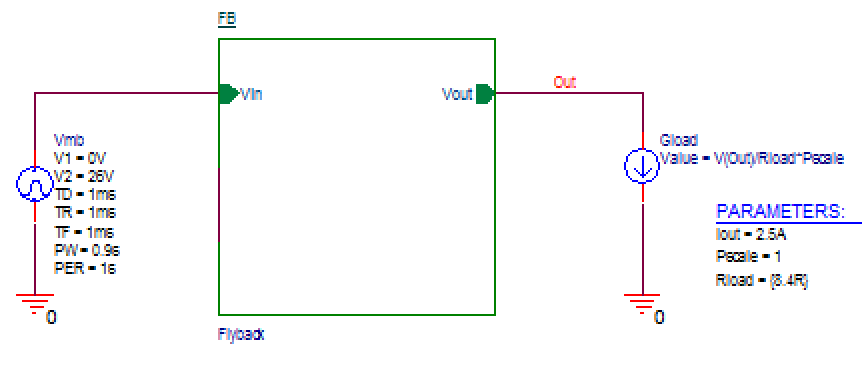
\includegraphics[max width=0.7\linewidth]{/tex/2iteration/billeder/Simulering_2iteration_top.png}
	\caption{Yderste blok af simulering}
	\label{fig: simtop}
\end{figure}
Imellem er blokken "Flyback". Heri er selve kredsløbet. Dykkes der ind i denne blok fås det der ses på figur~\ref{fig: simfly} 
\begin{figure}[H]
	\center
	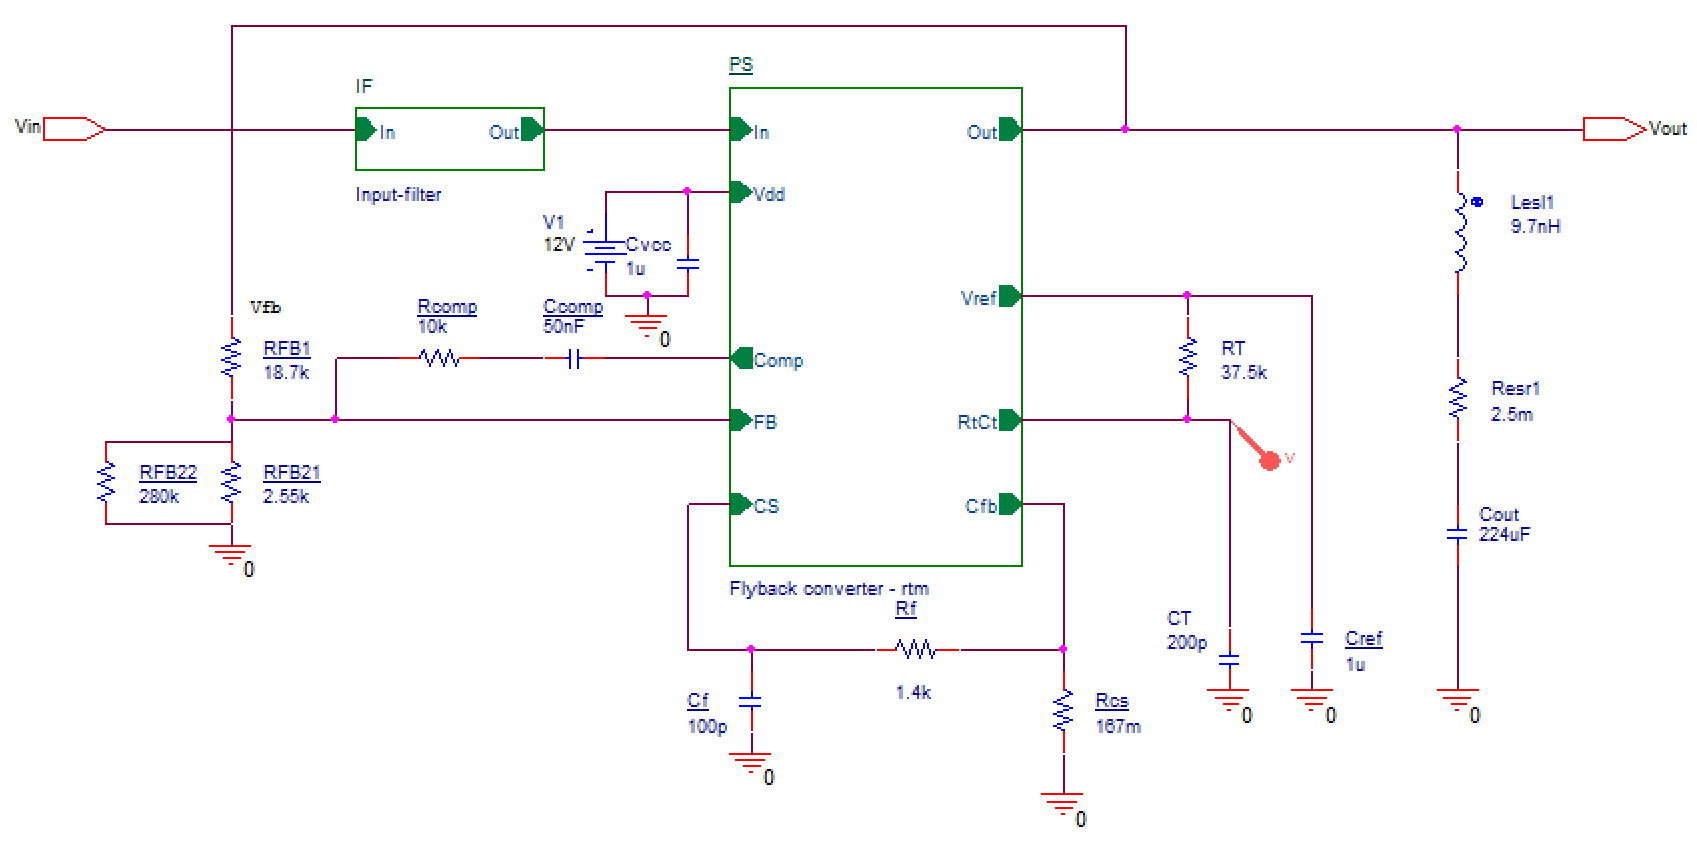
\includegraphics[max width=0.7\linewidth]{/tex/2iteration/billeder/Simulering_2iteration_flyback.png}
	\caption{Flyback blok}
	\label{fig: simfly}
\end{figure}
Her ses yderligere 2 blokke hhv. Inputfilter og flyback converter. Ud over disse blokke ses de komponenter, der er brugt til at få PWM controlleren til at køre efter hensigten. Selve controlleren ligger inde i flyback converter blokken. Værdierne og forklaringen af komponenterne blev gennemgået i analyse afsnittet om PWM controlleren??
Desuden ses output kondensatoren med de udregnede parasitter også.


\noindent Blokken for inputfiltret er allerede vist tidligere under forklaringen af denne, så den vises ikke igen. Til gengæld ses indholdet af Flyback converter blokken på figur~\ref{fig: simflycon}. 
\begin{figure}[H]
	\center
	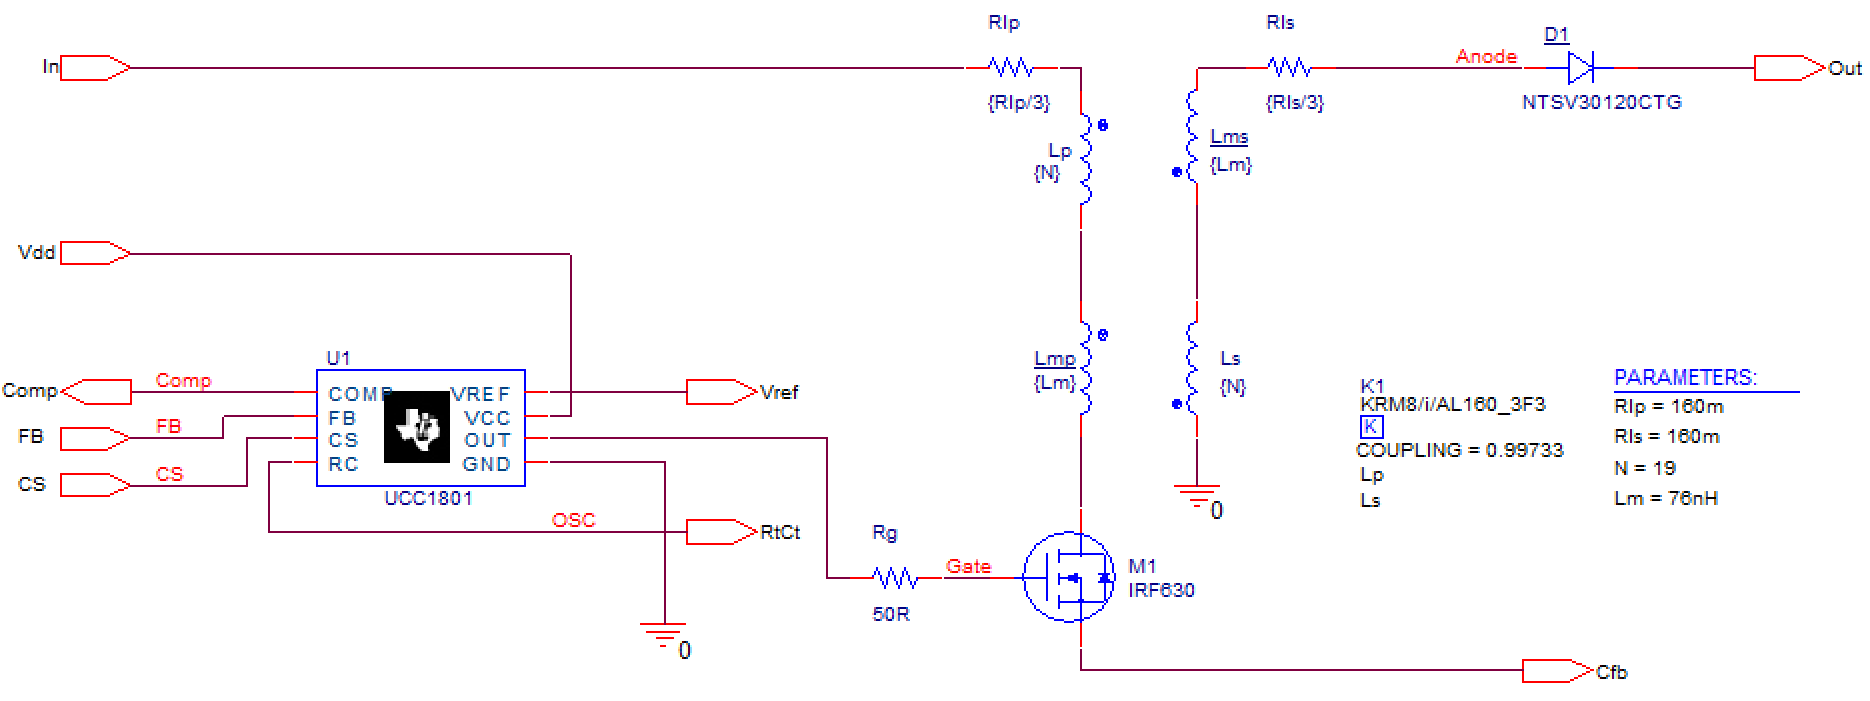
\includegraphics[max width=0.7\linewidth]{/tex/2iteration/billeder/Simulering_2iteration_flycon.png}
	\caption{Flyback converter blok}
	\label{fig: simflycon}
\end{figure}
Heri ses selve PWM controlleren UCC1801, som der er trukket en model ind for. \cite{??}. Også MOSFET'en og Dioden er der trukket modeller ind for. Ved MOSFET'en har det ikke været muligt at finde den præcise model. Derfor er IRF630 modellen istedet brugt, da det er vurderet, at den minder en del om den. \cite{IRF630MOSFET} 
Yderligere ses transformatoren, hvor både spredningsselvinduktion og kobbermodstanden i ledningerne er tegnet med samt kernemodellen for 3F3 er trukket ind.

\subsection{Constant load}
Ved constant load simuleringen simuleres ved en load på $8.4\ohm$, efter $20ms$ så det sikres, at der ses på den stationære udgang. Indgangsspændingen er sat til 26V.
Første plot af denne simulering ses på figur~\ref{fig: simflycon}. Her ses både strøm og spænding på udgangen.
\begin{figure}[H]
	\center
	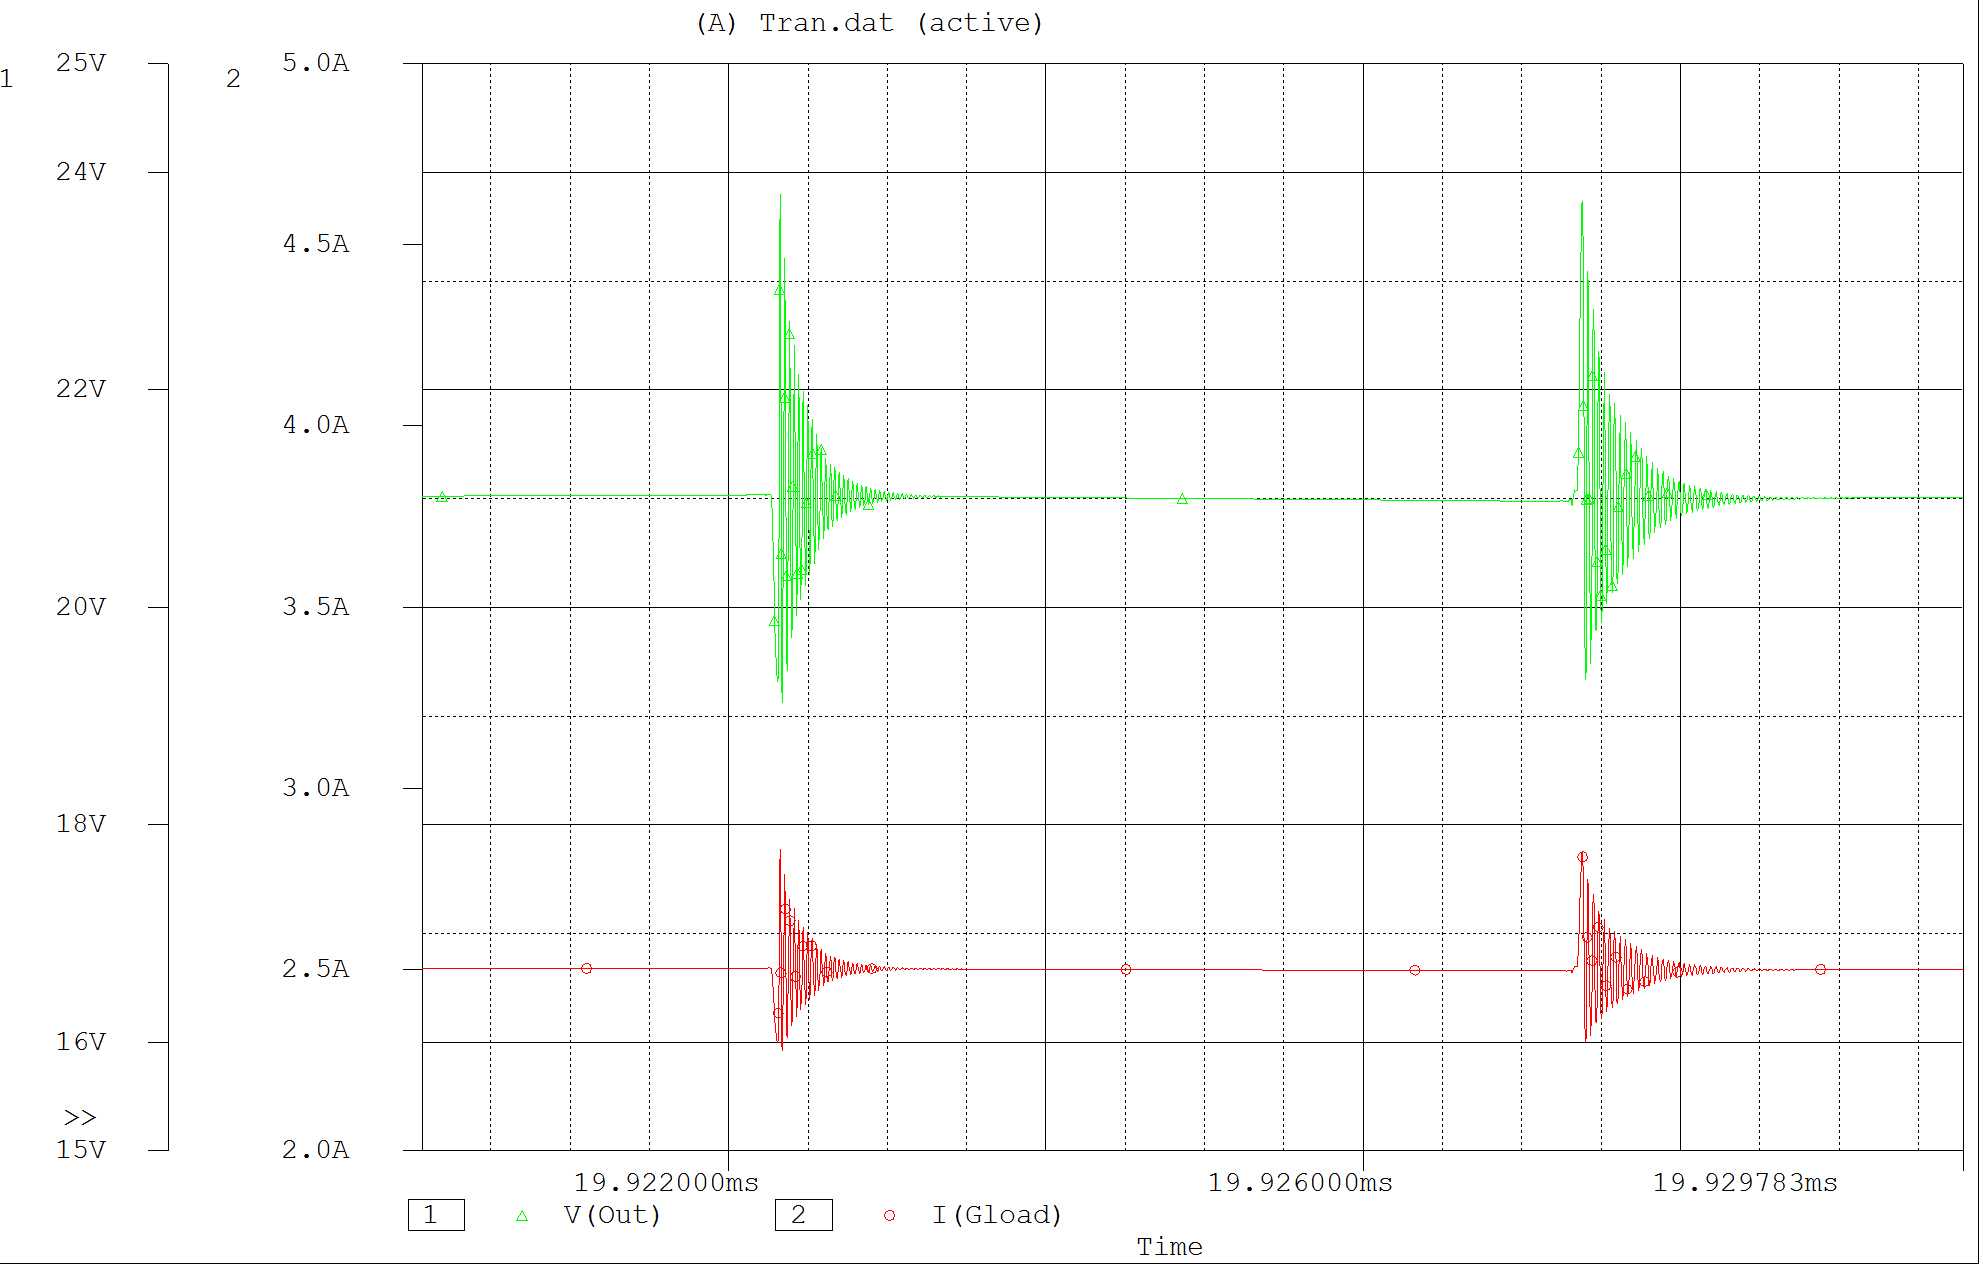
\includegraphics[max width=0.7\linewidth]{/tex/2iteration/billeder/Simudgang.png}
	\caption{Simulering af udgang}
	\label{fig: simudgang}
\end{figure}
Her ses det at spændingen V(out) ligger på 21V, dog med svingninger hver gang der switches. Det ser altså ud til at switching transienter fra MOSFET og diode kommer til syne på udgangen. Det er samme billede for strømmen I(Gload), der ellers ligger på de forventede 2.5A.

På figur~\ref{fig: simMOSdio} ses en spændingsperiode for drain benet på MOSFET'en samt dioden. 
\begin{figure}[H]
	\center
	\includegraphics[max width=0.7\linewidth]{/tex/2iteration/billeder/SIMMOSFETdiode.png}
	\caption{Simulering af spænding over diode og drain ben på MOSFET}
	\label{fig: simMOSdio}
\end{figure}
Det ses, at når transistoren (rød kurve) går off så kommer den tidligere omtalte peakspænding samt den svinger, inden den går til en stationær værdi på ca. 48V, inden MOSFET'en switches on igen. Dette stemmer fint overens med analysen hvor den stationær værdi bør ligge på 21V+26V=47V.
Peak'en er ca. 93V.
Det samme ses for dioden (grøn kurve) at når transistoren er on, vil dioden ikke være i lederetningen, og skal derfor kunne holde til den peak på ca. 80V der ses på grafen. Derudover lægger den sig på en stationær værdi på ca. 46V, hvilket igen stemmer pænt overens med de 47V.

\clearpage 

\section{Realisering}
I dette afsnit implementeres, og testes, den designede converter i anden iteration. Implementeringen sker på et Mini-Mount, som består af et stort ground plan. Selve banerne består af små PCB-stykker der klistres ovenpå, hvor komponenterne loddes på. Ground plannet giver optimale forhold for både strømveje og afkobling. Da det er essentielt at holde banerne til ground på det minimale, giver ground planet de bedst mulige betingelser for converteren. 

Mini-Mount'et ses på figur~\ref{fig:Mini_Mount}. Inputspændingen til converteren er placeret i midten til højre, inputspændingen til PWM-controlleren er placeret nederst til højre, og udgangen til loaden er placeret øverst til venstre. Med mindre andet er beskrevet testes der med fuld belastning ved $8.4\ohm$.

\begin{figure}[H]
	\center
	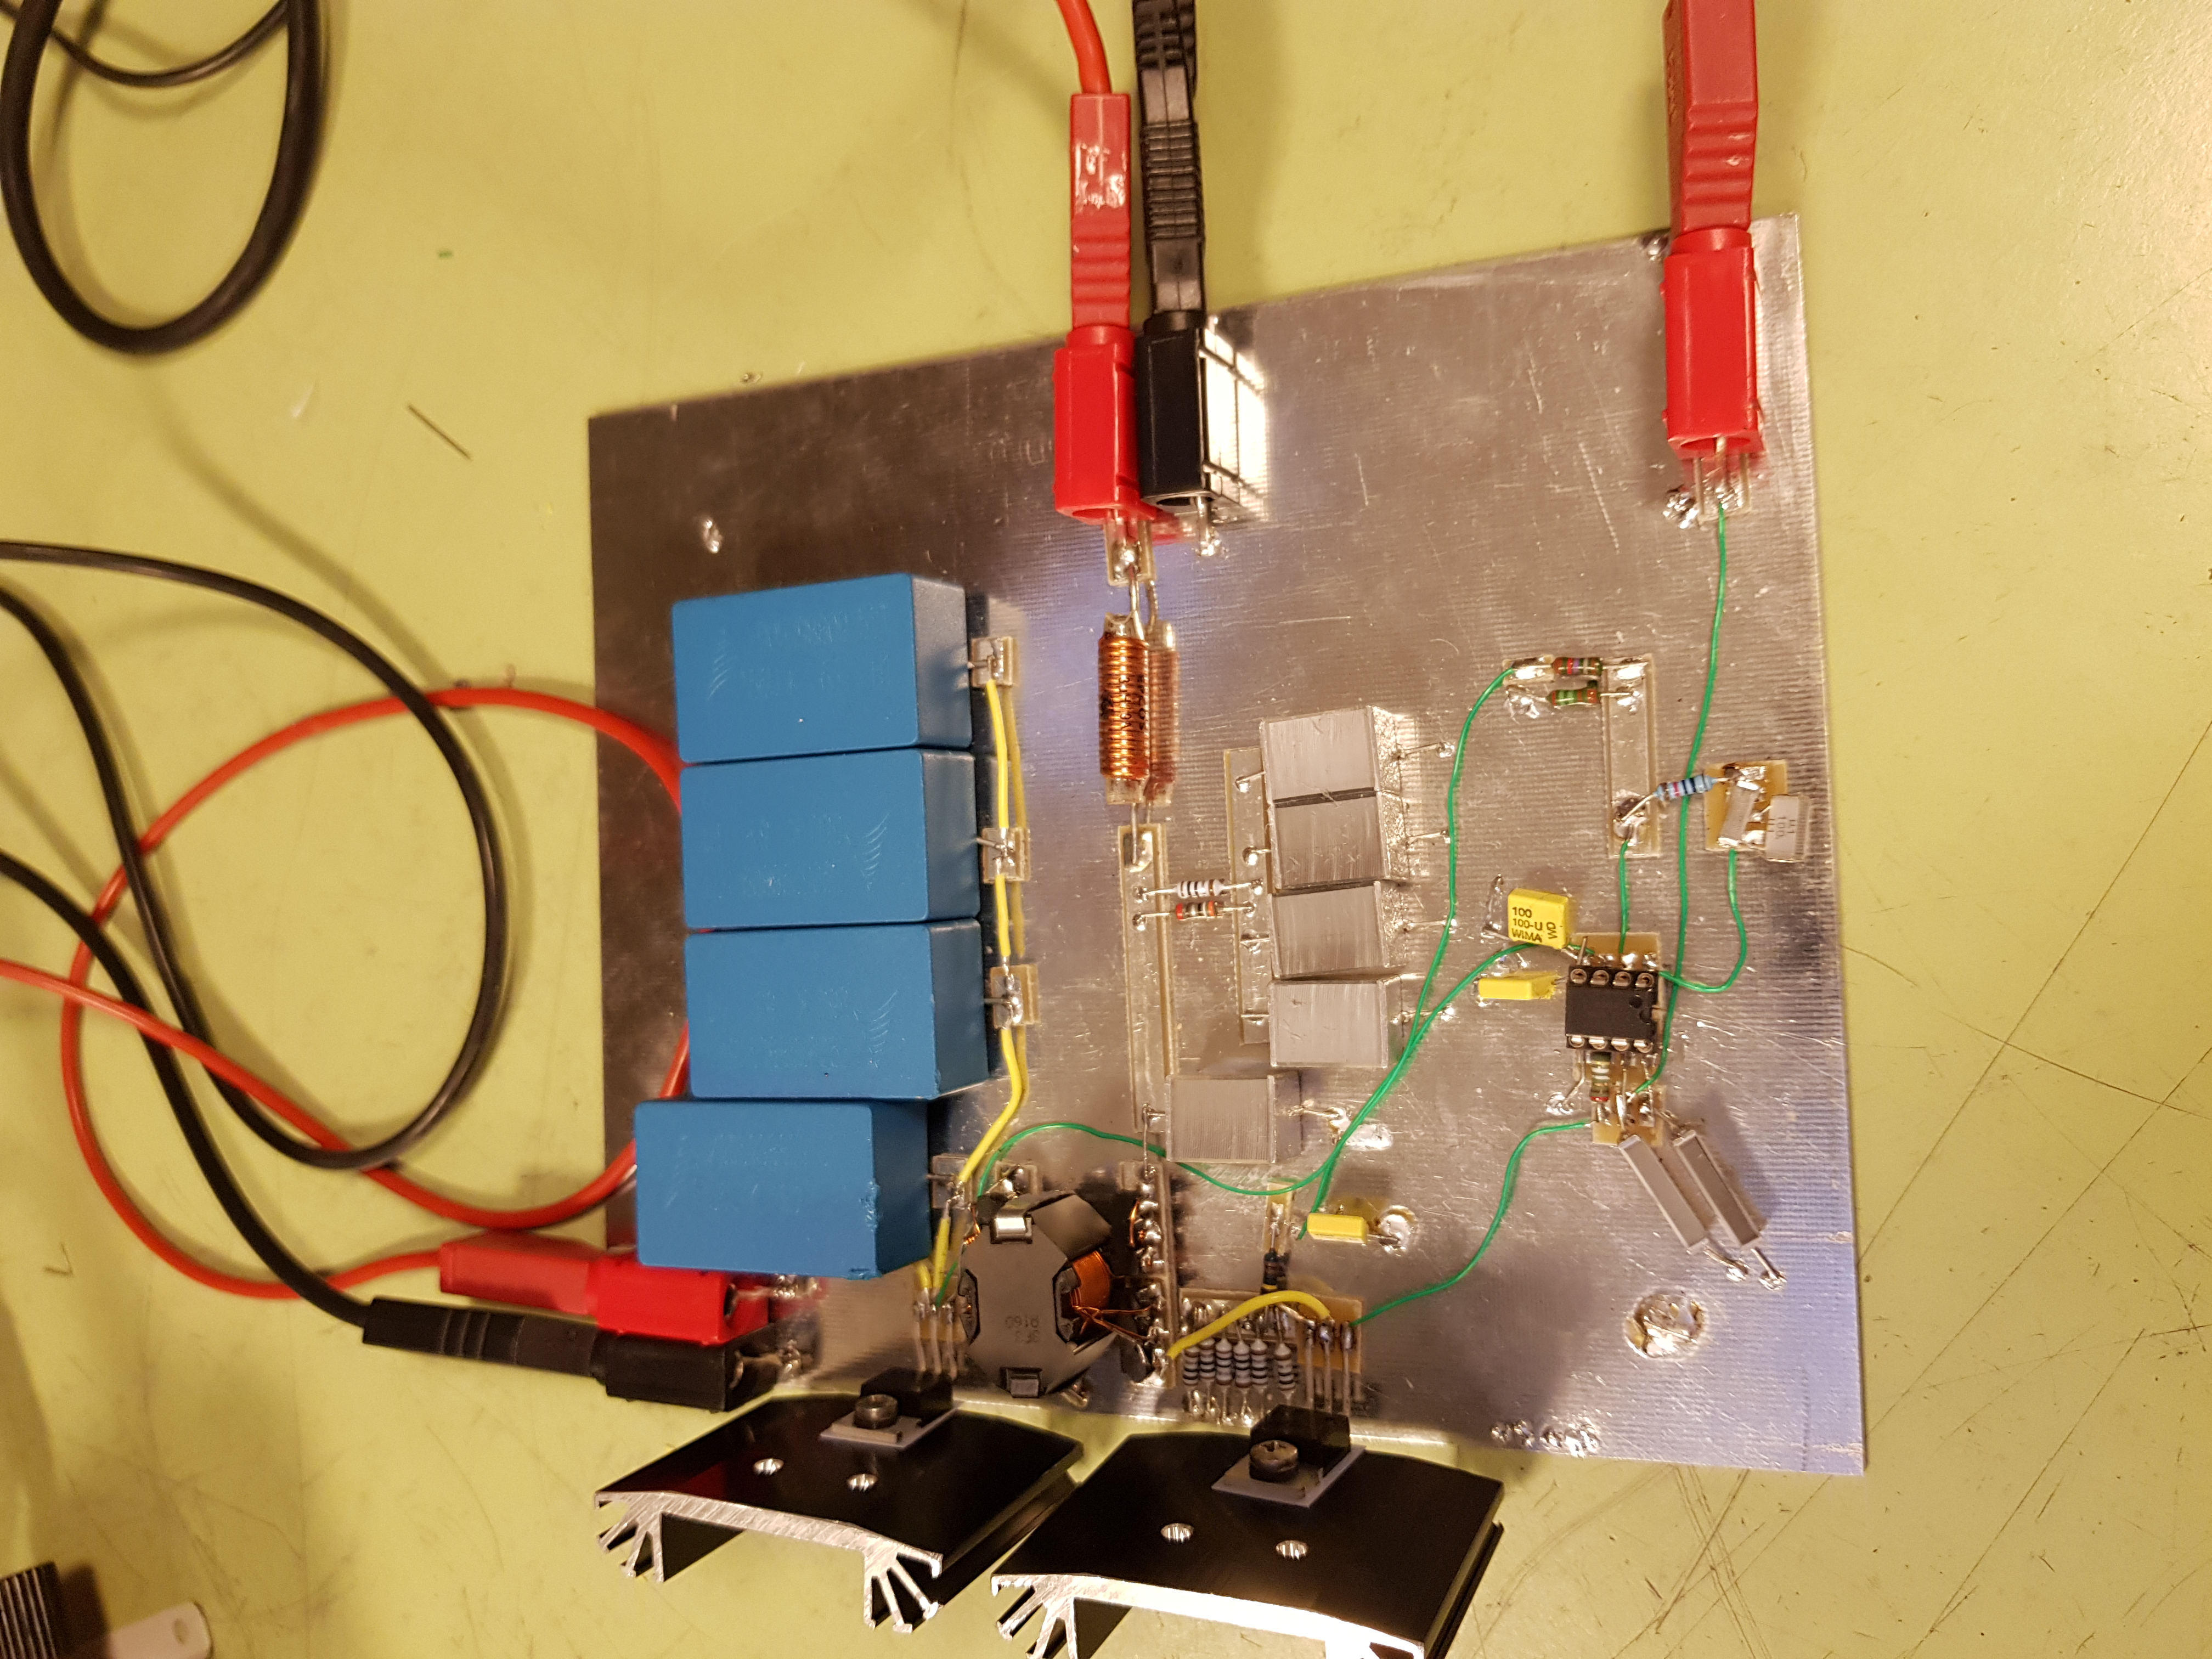
\includegraphics[max width=0.7\linewidth, angle=-90]{/tex/2iteration/billeder/Realisering/Print.JPG}
	\caption{Mini-Mount af converter}
	\label{fig:Mini_Mount}
\end{figure}

%%% Realisering af PWM controller %%%

\subsection{PWM-controller}
I det følgende afsnit testes implementeringen af PWM-controlleren. Her måles frekvensen af savtandspændingen og selve switch-frekvensen, samt signalet over current-sense modstanden både før og efter filteret.

\subsubsection{Switch-frekvens}
Først måles frekvensen af savtandspændingen. Denne frekvens måles til $160k\hertz$, hvor der ønskes $200k\hertz$. Da switch-frekvensen af indflydelse på mange ting i converteren, ændres modstanden således der opnås en frekvens på ca. $200k\hertz$. Der vælges en modstand på $33.2k\ohm$. På figur~\ref{fig:Savtand} og \ref{fig:Udgang_PWM} ses henholdsvis målingen af savtandspændingen og udgangen af PWM-controlleren. Her ses det, at der er opnået en frekvens for savtandspændingen på $192k\hertz$, og en frekvens for udgangssignalet på $102.6k\hertz$. Med et udgangspunkt på $100k\hertz$, godtages denne afvigelse. Resultaterne for analyse, simulering og realisering indføres i tabel~\ref{tab:resultat_switch_frekvens}.


\begin{table}[H] 			
	\centering
	\begin{tabularx}{\textwidth}{|X|c|c|c|}
		\hline
		\textbf{Frekvens} & \multicolumn{3}{|c|}{\textbf{Oscillator frekvens}} 										\\ \hline
		& A & S & R 									\\ \hline
		$f_{osc}$ & $200k\hertz$ & $199.6k\hertz$ & $192k\hertz$ 									\\ \hline 
		$f_s$ & $100k\hertz$ & $99.01k\hertz$ & $102.6k\hertz$ 									\\ \hline
	\end{tabularx}
	\caption{Resultater for analyse, simulering og realisering af switch-frekvens}
	\label{tab:resultat_switch_frekvens}
\end{table}


\begin{figure}[H]
	\center
	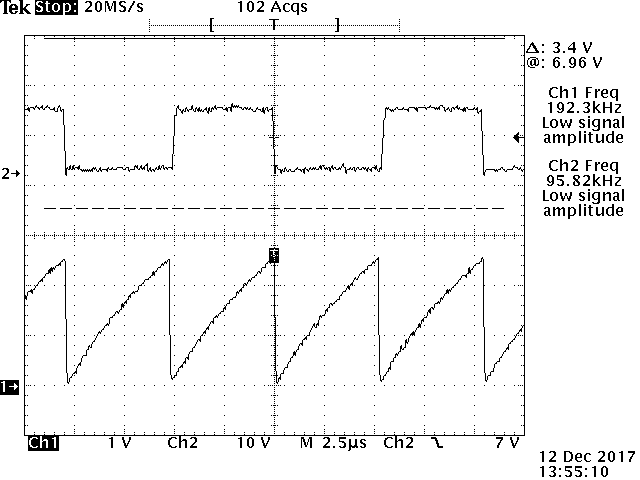
\includegraphics[max width=0.7\linewidth]{/tex/2iteration/billeder/Realisering/Savtand.png}
	\caption{Måling af savtandspænding}
	\label{fig:Savtand}
\end{figure} 

\begin{figure}[H]
	\center
	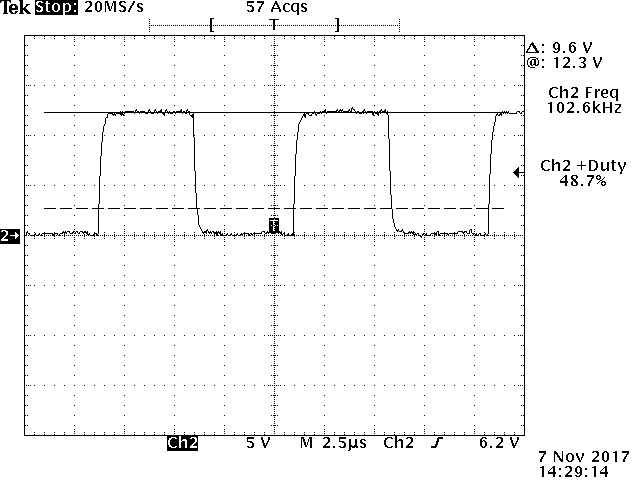
\includegraphics[max width=0.7\linewidth]{/tex/2iteration/billeder/Realisering/Udgang_PWM.png}
	\caption{Udgang af PWM-controller}
	\label{fig:Udgang_PWM}
\end{figure} 

\subsubsection{Switch-tid}
Målingen af switch-tiden er vist på figur~\ref{fig:Realisering_MOSFET_switch_tid_2}. Figuren viser MOSFET'ens drain på kannal 1, og MOSFET'ens gate på kannal 2. Her aflæses switch-tiden i MOSFET'en som længden af plateauet på gate signalet, og aflæses til ca. $120ns$. Resultaterne for analyse, simulering og realisering er indført i tabel~\ref{tab:resultat_switch_tid_2}. Her er simuleringen dog foretaget med en anden MOSFET.

\begin{table}[H] 			
	\centering
	\begin{tabularx}{\textwidth}{|X|c|c|c|}
		\hline
		\textbf{Tid} & \multicolumn{3}{|c|}{\textbf{Switch-tid}} 										\\ \hline
		& A & S & R 									\\ \hline
		$T_{ch}$ & $138.7ns$ & $103ns$ & $120ns$ 									\\ \hline 
		
	\end{tabularx}
	\caption{Resultater for analyse, simulering og realisering af switch-tid}
	\label{tab:resultat_switch_tid_2}
\end{table}

 
\begin{figure}[H]
	\center
	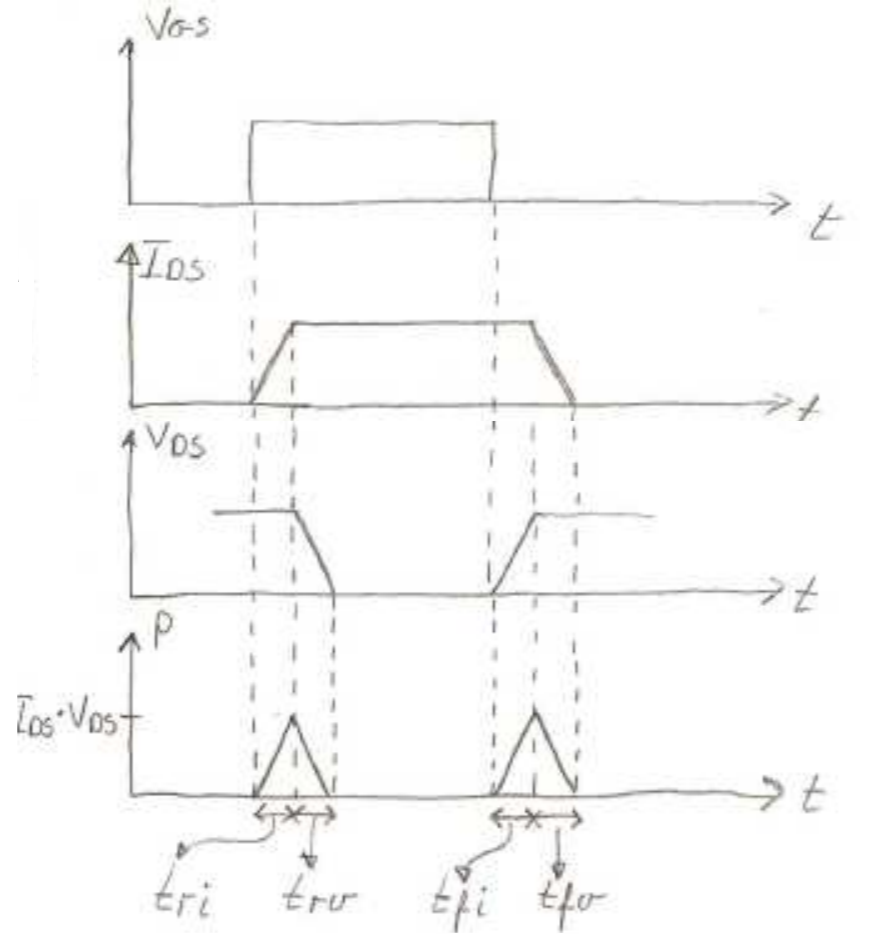
\includegraphics[max width=0.7\linewidth]{/tex/2iteration/billeder/Realisering/MOSFET_switch_tid.png}
	\caption{Switch-tid for MOSFET'en}
	\label{fig:Realisering_MOSFET_switch_tid_2}
\end{figure} 


\subsubsection{Current-sense kredsløb}
Current-sense signalet måles både før og efter filteret. Signalet før filteret ses på figur~\ref{fig:CS_U_filter}. Her ses tydeligt de spikes der ønskes filtreret væk, da de overstiger den egentlige peak på signalet. Figur~\ref{fig:CS_M_filter} viser signalet efter filteret. Her ses det at de spikes der var på signalet er blevet filtreret væk. Til gengælder ses det at signalet er blevet langsommere, ved de afrundede hjørner. Dette er ikke optimalt ved lavere duty-cycles, da det som nævnt i afsnit~\ref{CS_protection} vil påvirke systemets I/V-karakteristik. Derfor vil stige tiden af filteret blive optimeret i tredje iteration. 

\begin{figure}[H]
	\center
	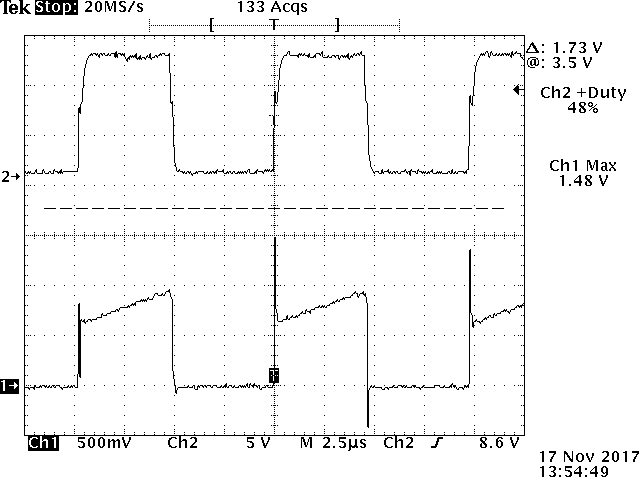
\includegraphics[max width=0.7\linewidth]{/tex/2iteration/billeder/Realisering/CS_U_filter.png}
	\caption{Current-sense signal før filter}
	\label{fig:CS_U_filter}
\end{figure}

\begin{figure}[H]
	\center
	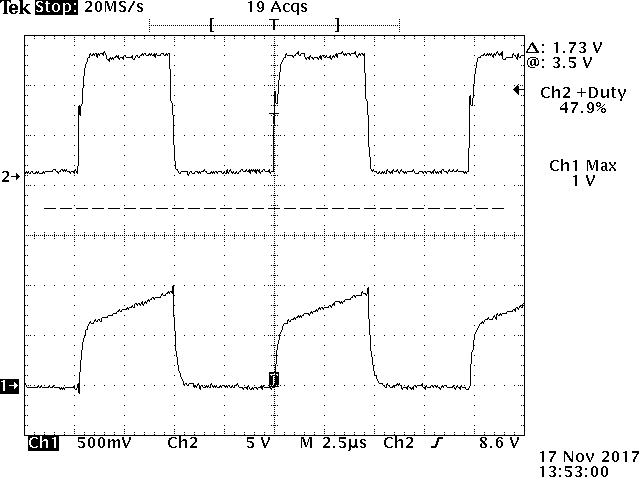
\includegraphics[max width=0.7\linewidth]{/tex/2iteration/billeder/Realisering/CS_M_filter.png}
	\caption{Current-sense signal efter filter}
	\label{fig:CS_M_filter}
\end{figure}


\subsubsection{Spændingsdeler}
Spændingsdeleren testes ved at måle indgangsspændingen til fejlforstærkeren, når udgangsspændingen er $21V$. Dette er gjort på figur. Spændingen er målt til $2.5V$. Resultaterne for analyse, simulering og realisering er indført i tabel~\ref{label}.

\begin{table}[H] 			
	\centering
	\begin{tabularx}{\textwidth}{|X|c|c|c|}
		\hline
		\textbf{Spænding} & \multicolumn{3}{|c|}{\textbf{Resultater}} 		\\ \hline
		& A & S & R 									\\ \hline
		$V_{FB}$ & $2.5V$ & $103ns$ & $120ns$ 									\\ \hline 
		
	\end{tabularx}
	\caption{Resultater for analyse, simulering og realisering af switch-tid}
	\label{tab:resultat_voltage_divider}
\end{table}

\subsubsection{Constant load}
Ligesom ved simuleringsafsnittet ~\ref{constant} ses der på spænding på både udgang og begge sider af transformatoren. Der er brugt en indgangsspænding på 26V og en load på $8.4\ohm$. 
Først er scoopets proper sat henover udgangen og resultatet af dette se på figur~\ref{fig: Out26V}
\begin{figure}[H]
	\center
	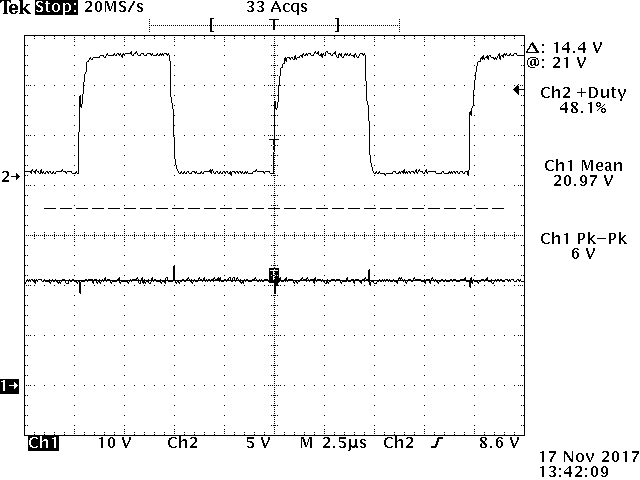
\includegraphics[max width=0.7\linewidth]{/tex/2iteration/billeder/Realisering/Output_filtreret_26V.png}
	\caption{Spændingsoutput ved 26V}
	\label{fig: Out26V}
\end{figure}
Det ses at spændingen ligger på 20.97V, altså de forventede 21V. Der kan dog identificeres nogle ret store spikes. På figur~\ref{fig: Out26Vzoom} er der zoomet ind på disse.
\begin{figure}[H]
	\center
	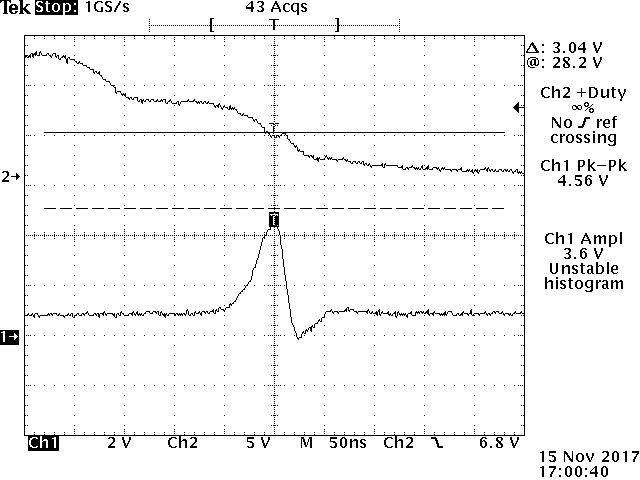
\includegraphics[max width=0.7\linewidth]{/tex/2iteration/billeder/Realisering/Outputspike_zoom.png}
	\caption{Zoomet på outputspike}
	\label{fig: Out26Vzoom}
\end{figure}
Her ses det, at spiken når helt op på en peak af 4,5V. Disse peaks skyldes switching transienter og ved figur~\ref{fig: Out26V} kan det også ses, at det sker hver gang transistoren går on eller off.

Disse transienter er endnu tydeligere ved transformatorens primær- og sekundærvikling. Først ses på figur~\ref{fig: privolt} spændingen ved den primærevikling. Det svarer til spændingen over drain på MOSFET'en. 
\begin{figure}[H]
	\center
	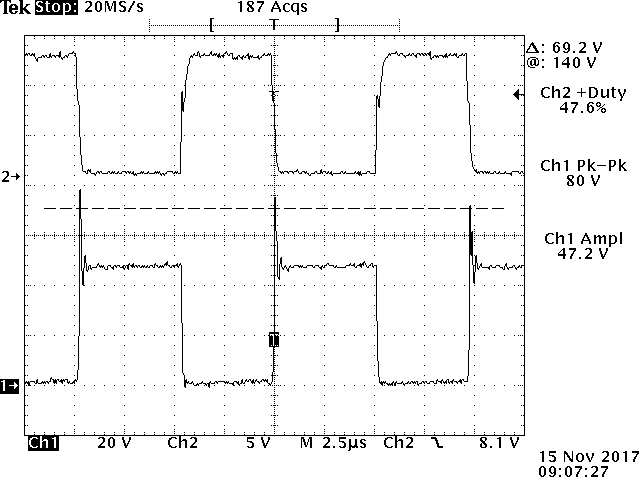
\includegraphics[max width=0.7\linewidth]{/tex/2iteration/billeder/Realisering/Transformator_Primar.png}
	\caption{Primær spænding}
	\label{fig: privolt}
\end{figure}
Det ses, at spændingen stiger med et stort peak på 80V, når transistoren går off, og ligger sig stationært på ca. 47V og falder til 0V igen, når transistoren går on. På figur~\ref{fig: prizoom} zoomes der ind på spiken.
\begin{figure}[H]
	\center
	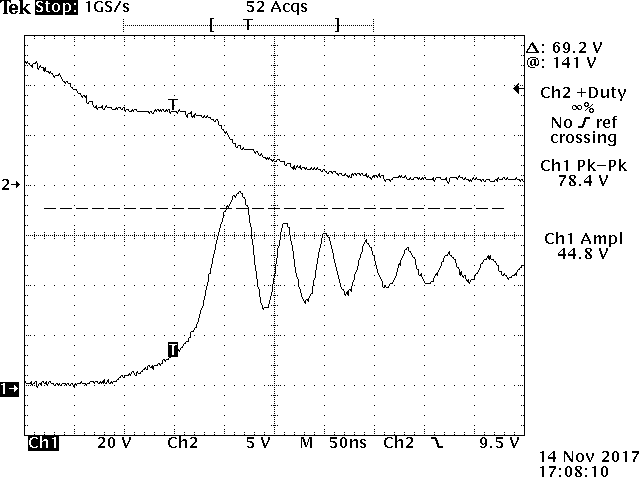
\includegraphics[max width=0.7\linewidth]{/tex/2iteration/billeder/Realisering/Transformator_Primarzoom.png}
	\caption{Zoomet på primær peak}
	\label{fig: prizoom}
\end{figure}
Udover peaken ses det, at spændingen svinger inden den ligger sig på den stationære værdi. Ses der på 2. svingningsperiode, aflæses svingningen for en periode til 40ns. Det betyder at frekvensen der ses ligger på ca:
\begin{equation} \label{svingpri}
f_{oscpri} = \frac{1}{40ns} = 25MHz
\end{equation}

På samme måde ses der på figur~\ref{fig:sek} på spændingen over den sekundære vikling. Det svarer også til spændingen på anoden af dioden. 
\begin{figure}[H]
	\center
	\includegraphics[max width=0.7\linewidth]{/tex/2iteration/billeder/Realisering/Transformator_sekundar.png}
	\caption{Sekundær spænding}
	\label{fig:sek}
\end{figure}
Her falder spændingen, når transistoren går on, og falder i første omgang med ca. 60V. Herefter ligger den på ca. 45V indtil transistoren går off og spændingen ligger sig på 20V med et mindre peak. På figur~\ref{fig:sekzoom} zoomes der ind på peaken hvor transistoren går on.
\begin{figure}[H]
	\center
	\includegraphics[max width=0.7\linewidth]{/tex/2iteration/billeder/Realisering/Transformator_sekundarzoomrise.png}
	\caption{Zoomet på sekundær peak}
	\label{fig:sekzoom}
\end{figure}
Igen observeres det, at spændingen svinger indtil den når sin stationære værdi. Her aflæses svingningen til at være 35ns, og derfor lidt kortere end ved primærviklingen. Det giver en frekvens på:
\begin{equation} \label{svingsek}
f_{oscsek} = \frac{1}{35ns} = 28.57MHz
\end{equation}

I tabellen nedenfor ses en oversigt over simulering og realisering for drain spændingen på MOSFET'en samt anoden på dioden.

\begin{table}[H] 			
	\centering
	\begin{tabularx}{\textwidth}{|X|l|l|l|l|}
		\hline
		 & \multicolumn{2}{|X|}{\textbf{Simulering}} & \multicolumn{2}{|X|}{\textbf{Realisering}} \\ \hline
		 & MOSFET & Diode & MOSFET & Diode \\ \hline
		Stationær spænding & $48V$ & $46V$ & $47V$ & $45V$ \\ \hline
		Peakspænding & $93V$ & $80V$ & $80V$ & $60V$ \\ \hline
		Svingningsfrekvens & $29.41M\hertz$ & $33.33M\hertz$ & $25.00M\hertz$ & $28.57M\hertz$ \\ \hline
	\end{tabularx}
	\caption{Simulering og realisering af spændinger over MOSFET og diode}
	\label{tab:MOSDIODE}
\end{table}

\subsubsection{Load step}
Load steppet er realiseret på samme måde som det blev simuleret tidligere. Med 2 $20\ohm$ modstande i parallel. Den ene med en switch, så når switchen er off består loaden af en $20\ohm$ modstand, men når switchen går on er loaden $10\ohm$. Switchen blev indstillet til at sende en puls på 10ms. Oscilloskop propperne blev sat til at måle over udgangen, og resultatet af dette ses På figur~\ref{fig:belastning_samlet} 
\begin{figure}[H]
	\center
	\includegraphics[max width=0.7\linewidth]{/tex/2iteration/billeder/Realisering/belastningsamlet.png}
	\caption{Realisering af load step}
	\label{fig:belastningsamlet}
\end{figure}
Det ses hvordan spændingen falder først hvor belastningen stiger til $10\ohm$ og efter 10ms stiger spændingen, hvor belastningen kommer tilbage tl de $20\ohm$. På figur~\ref{fig:belastning_10ohm} er der zoomet ind på dykket ved de 10 ohm. 
\begin{figure}[H]
	\center
	\includegraphics[max width=0.7\linewidth]{/tex/2iteration/billeder/Realisering/belastningstiger(10ohm).png}
	\caption{Zoom på dyk ved 10ohm}
	\label{fig:belastning_10ohm}
\end{figure}
Det kan aflæses at spændingen når at falde med ca. $700mV$ og det tager ca. $1.5ms$ at regulere tilbage igen.

På samme måde ses stigningen ved de $20\ohm$ på figur~\ref{fig:belastning_20ohm}
\begin{figure}[H]
	\center
	\includegraphics[max width=0.7\linewidth]{/tex/2iteration/billeder/Realisering/belastningfalder(20ohm).png}
	\caption{Zoom på stigning ved 20ohm}
	\label{fig:belastning_20ohm}
\end{figure}
Her stiger spændingen med ca. $600mV$ og bruger også omkring $1.5ms$ på at regulere ind igen. 

Nedenfor ses et overblik over simuleringen af load steppet i forhold til realiseringen. 

\begin{table}[H] 			
	\centering
	\begin{tabularx}{\textwidth}{|X|l|l|l|l|}
		\hline
		& \multicolumn{2}{|l|}{\textbf{Simulering}} & \multicolumn{2}{|l|}{\textbf{Realisering}} \\ \hline
		\textbf{Belastning} & $10\ohm$ & $20\ohm$ & $10\ohm$ & $20\ohm$ \\ \hline
		Overshoot & $650mV$ & $700mV$ & $700mV$ & $600mV$  \\ \hline
		Reguleringstid & $1.6ms$ & $1.6ms$ & $1.5ms$ & $1.5ms$ \\ \hline
	\end{tabularx}
	\caption{Simulering og realisering af load step}
	\label{tab:Loadstep}
\end{table}
Det ses at simulering og realisering stemmer godt overens. Da der både ved simulering og realisering aflæses på kurver, kan usikkerheden ved det skyldes den lille afvigelse.

\subsection{Gain-fase måling} \label{gain_fase_2}
Gain-fase målingen deles op i tre, ligesom ved analysen og simuleringen. Der måles overføringsfunktion for power modulet, fejlforstærkeren, og for det samlede system. Målingerne foretages vha. en Network Analyzer af typen HP4194A. Den måler overføringsfunktionen ved at indførere et fejlsignal i tilbagekoblingen, og måle hvordan udgange ændre sig. Derved opnås åbensløjfe overføringsfunktionen. Som ved simuleringen indføres fejlsignalet over en $51.1\ohm$ modstand, placeret i serie med den første modstand i spændingsdeleren. 

Amplituden af fejlsignalet vælges til $30mV$. Ved for lille en amplitude kan signal/støj forholdet blive for småt ved lave frekvenser, mens en stor amplitude kan overstyre fejlforstærkeren. Ud fra Termas erfaringer er $30mV$ et fint udgangspunkt, men den skal muligvis justeres senere. For frekvens-sweepet vælges der et logaritmisk sweep, mens startfrekvensen vælges til $10\hertz$, og slutfrekvensen vælges til $100k\hertz$. 

Først måles gain-fasen for selve power modulet. Det gøres ved at måle mellem udgangen fra fejlforstærkeren, og udgangen fra converteren. Det er vist på figur~\ref{fig:realisering_gain_fase_power}. Der vist bode plot for både analyse og realisering. På grund af usikkerhed i simuleringen er denne del udeladt. Gain for realiseringen er den blå, mens gain for analysen er den grønne stiplede. Fasen for realiseringen er er den røde, mens fasen for analysen er den stiplede lilla. Det ses at gain-fase karakteristikken ser ud som forventet ud fra analysen. Det er først ved de høje frekvenser målingen afviger fra analysen. Båndbredden for power modulet aflæses til ca. $1400\hertz$, mens DC-gain aflæses til ca. $20.3\decibel$.

\begin{figure}[H]
	\center
	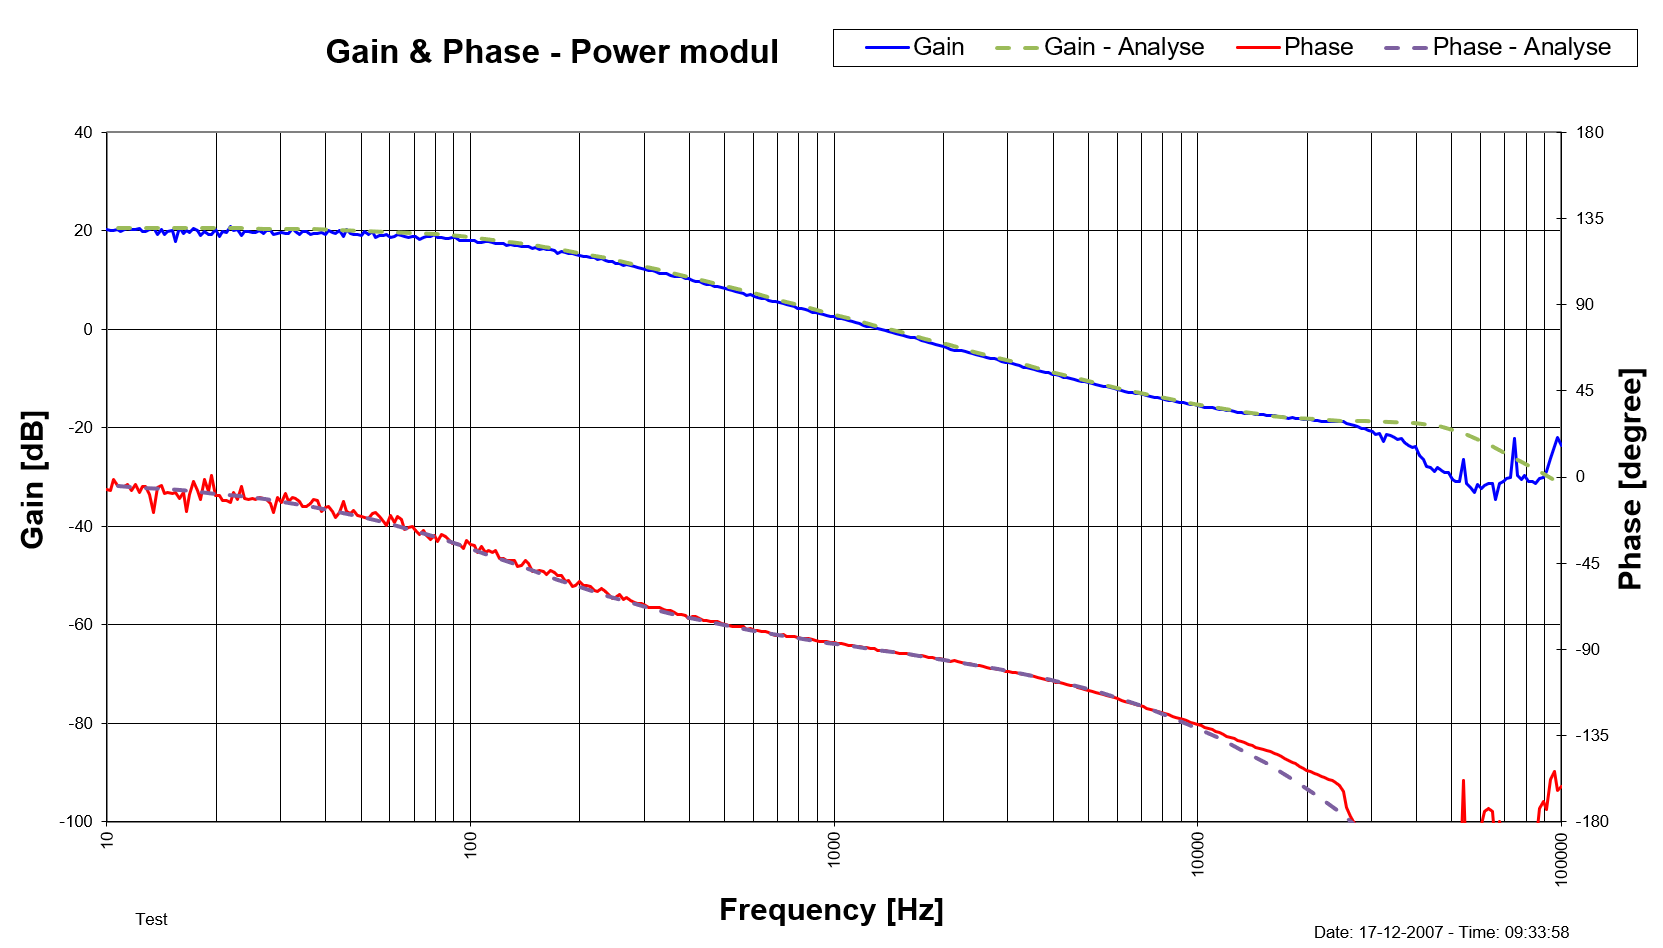
\includegraphics[max width=0.7\linewidth]{/tex/2iteration/billeder/Realisering/Realisering_gain_fase_power.png}
	\caption{Realisering af gain-fase for power modul}
	\label{fig:realisering_gain_fase_power}
\end{figure}

%TODO: Beskriv fejlforstærker når målinger hentes ved Terma


Til sidst måles den samlede overføringsfunktion for systemet. Her måles der over den modstand, hvor fejlsignalet indføres. Det svarer til at måle fra indgangen af fejlforstærkeren til udgangen af converteren. Bode plottet for både analyse og realiseringen er vist på figur~\ref{fig:realisering_gain_fase_tot}. Gain for realiseringen er den blå, mens gain for analysen er den grønne stiplede. Fasen for realiseringen er er den røde, mens fasen for analysen er den stiplede lilla. På bode plottet ses det at der er en smule større afvigelse, både ved gain og fasen. På trods af afvigelsen aflæses båndbredden dog nogenlunde til det samme på ca. $900\hertz$. Fase-margin aflæses til ca. $62^\circ$, og gain-margin aflæses til ca. $24\decibel$. Holdt op mod analysen var det forventet at opnå en fase-margin på $74.3^\circ$ og en gain-margin på $24\decibel$. Afvigelsen i fase-margin ses på figur~\ref{fig:realisering_gain_fase_tot}, da den faktiske fase ligger under den analyserede. 

\begin{figure}[H]
	\center
	\includegraphics[max width=0.7\linewidth]{/tex/2iteration/billeder/Realisering/Realisering_gain_fase_tot.png}
	\caption{Realisering af gain-fase for hele systemet}
	\label{fig:realisering_gain_fase_tot}
\end{figure}

















